\documentclass[twoside]{book}

% Packages required by doxygen
\usepackage{fixltx2e}
\usepackage{calc}
\usepackage{doxygen}
\usepackage[export]{adjustbox} % also loads graphicx
\usepackage{graphicx}
\usepackage[utf8]{inputenc}
\usepackage{makeidx}
\usepackage{multicol}
\usepackage{multirow}
\PassOptionsToPackage{warn}{textcomp}
\usepackage{textcomp}
\usepackage[nointegrals]{wasysym}
\usepackage[table]{xcolor}

% Font selection
\usepackage[T1]{fontenc}
\usepackage[scaled=.90]{helvet}
\usepackage{courier}
\usepackage{amssymb}
\usepackage{sectsty}
\renewcommand{\familydefault}{\sfdefault}
\allsectionsfont{%
  \fontseries{bc}\selectfont%
  \color{darkgray}%
}
\renewcommand{\DoxyLabelFont}{%
  \fontseries{bc}\selectfont%
  \color{darkgray}%
}
\newcommand{\+}{\discretionary{\mbox{\scriptsize$\hookleftarrow$}}{}{}}

% Page & text layout
\usepackage{geometry}
\geometry{%
  a4paper,%
  top=2.5cm,%
  bottom=2.5cm,%
  left=2.5cm,%
  right=2.5cm%
}
\tolerance=750
\hfuzz=15pt
\hbadness=750
\setlength{\emergencystretch}{15pt}
\setlength{\parindent}{0cm}
\setlength{\parskip}{3ex plus 2ex minus 2ex}
\makeatletter
\renewcommand{\paragraph}{%
  \@startsection{paragraph}{4}{0ex}{-1.0ex}{1.0ex}{%
    \normalfont\normalsize\bfseries\SS@parafont%
  }%
}
\renewcommand{\subparagraph}{%
  \@startsection{subparagraph}{5}{0ex}{-1.0ex}{1.0ex}{%
    \normalfont\normalsize\bfseries\SS@subparafont%
  }%
}
\makeatother

% Headers & footers
\usepackage{fancyhdr}
\pagestyle{fancyplain}
\fancyhead[LE]{\fancyplain{}{\bfseries\thepage}}
\fancyhead[CE]{\fancyplain{}{}}
\fancyhead[RE]{\fancyplain{}{\bfseries\leftmark}}
\fancyhead[LO]{\fancyplain{}{\bfseries\rightmark}}
\fancyhead[CO]{\fancyplain{}{}}
\fancyhead[RO]{\fancyplain{}{\bfseries\thepage}}
\fancyfoot[LE]{\fancyplain{}{}}
\fancyfoot[CE]{\fancyplain{}{}}
\fancyfoot[RE]{\fancyplain{}{\bfseries\scriptsize Generated by Doxygen }}
\fancyfoot[LO]{\fancyplain{}{\bfseries\scriptsize Generated by Doxygen }}
\fancyfoot[CO]{\fancyplain{}{}}
\fancyfoot[RO]{\fancyplain{}{}}
\renewcommand{\footrulewidth}{0.4pt}
\renewcommand{\chaptermark}[1]{%
  \markboth{#1}{}%
}
\renewcommand{\sectionmark}[1]{%
  \markright{\thesection\ #1}%
}

% Indices & bibliography
\usepackage{natbib}
\usepackage[titles]{tocloft}
\setcounter{tocdepth}{3}
\setcounter{secnumdepth}{5}
\makeindex

% Hyperlinks (required, but should be loaded last)
\usepackage{ifpdf}
\ifpdf
  \usepackage[pdftex,pagebackref=true]{hyperref}
\else
  \usepackage[ps2pdf,pagebackref=true]{hyperref}
\fi
\hypersetup{%
  colorlinks=true,%
  linkcolor=blue,%
  citecolor=blue,%
  unicode%
}

% Custom commands
\newcommand{\clearemptydoublepage}{%
  \newpage{\pagestyle{empty}\cleardoublepage}%
}

\usepackage{caption}
\captionsetup{labelsep=space,justification=centering,font={bf},singlelinecheck=off,skip=4pt,position=top}

%===== C O N T E N T S =====

\begin{document}

% Titlepage & ToC
\hypersetup{pageanchor=false,
             bookmarksnumbered=true,
             pdfencoding=unicode
            }
\pagenumbering{roman}
\begin{titlepage}
\vspace*{7cm}
\begin{center}%
{\Large My Project }\\
\vspace*{1cm}
{\large Generated by Doxygen 1.8.11}\\
\end{center}
\end{titlepage}
\clearemptydoublepage
\tableofcontents
\clearemptydoublepage
\pagenumbering{arabic}
\hypersetup{pageanchor=true}

%--- Begin generated contents ---
\chapter{rt-\/depth-\/map}
\label{md_README}
\hypertarget{md_README}{}
realtime disparity calculation from a v4l2 video device with opencv for calibrated Z\+ED stereo cam or E\+LP dual lens cam.

{\bfseries dependencies}\+: libjpeg and opencv build with modules from \href{https://github.com/opencv/opencv_contrib}{\tt https\+://github.\+com/opencv/opencv\+\_\+contrib} 
\chapter{Hierarchical Index}
\section{Class Hierarchy}
This inheritance list is sorted roughly, but not completely, alphabetically\+:\begin{DoxyCompactList}
\item \contentsline{section}{Block\+Matcher}{\pageref{classBlockMatcher}}{}
\begin{DoxyCompactList}
\item \contentsline{section}{H\+W\+Matcher\+Disparity\+Coprocessor}{\pageref{classHWMatcherDisparityCoprocessor}}{}
\item \contentsline{section}{S\+W\+Matcher\+Konolige}{\pageref{classSWMatcherKonolige}}{}
\item \contentsline{section}{S\+W\+Semi\+Global\+Matcher}{\pageref{classSWSemiGlobalMatcher}}{}
\end{DoxyCompactList}
\item \contentsline{section}{dcx\+\_\+config}{\pageref{structdcx__config}}{}
\item \contentsline{section}{dcx\+\_\+device}{\pageref{structdcx__device}}{}
\item \contentsline{section}{dcx\+\_\+uio\+\_\+info}{\pageref{structdcx__uio__info}}{}
\item \contentsline{section}{dcx\+\_\+uio\+\_\+map}{\pageref{structdcx__uio__map}}{}
\item \contentsline{section}{Decoder\+Device}{\pageref{classDecoderDevice}}{}
\begin{DoxyCompactList}
\item \contentsline{section}{M\+J\+P\+E\+G\+Decoder\+Device}{\pageref{classMJPEGDecoderDevice}}{}
\end{DoxyCompactList}
\item \contentsline{section}{error\+\_\+mgr}{\pageref{structerror__mgr}}{}
\item \contentsline{section}{Estimator}{\pageref{classEstimator}}{}
\item \contentsline{section}{Estimator\+Cmd\+Line\+Parser}{\pageref{classEstimatorCmdLineParser}}{}
\item \contentsline{section}{exec\+\_\+time\+\_\+struct}{\pageref{structexec__time__struct}}{}
\item \contentsline{section}{hsv\+\_\+object\+\_\+ranges}{\pageref{structhsv__object__ranges}}{}
\item \contentsline{section}{vdma\+\_\+transfer\+\_\+dim}{\pageref{structvdma__transfer__dim}}{}
\item \contentsline{section}{Video\+Filter\+Device}{\pageref{classVideoFilterDevice}}{}
\begin{DoxyCompactList}
\item \contentsline{section}{H\+W\+Morphological\+Filter\+I\+P\+Core}{\pageref{classHWMorphologicalFilterIPCore}}{}
\item \contentsline{section}{S\+W\+Morphological\+Filter}{\pageref{classSWMorphologicalFilter}}{}
\end{DoxyCompactList}
\item \contentsline{section}{video\+Stream\+Buffer}{\pageref{structvideoStreamBuffer}}{}
\item \contentsline{section}{Video\+Stream\+Stereo\+Device}{\pageref{classVideoStreamStereoDevice}}{}
\begin{DoxyCompactList}
\item \contentsline{section}{V4\+L\+Stream\+Stereo\+Device}{\pageref{classV4LStreamStereoDevice}}{}
\end{DoxyCompactList}
\item \contentsline{section}{xmorph\+\_\+filter\+\_\+uio\+\_\+info}{\pageref{structxmorph__filter__uio__info}}{}
\item \contentsline{section}{xmorph\+\_\+filter\+\_\+uio\+\_\+map}{\pageref{structxmorph__filter__uio__map}}{}
\end{DoxyCompactList}

\chapter{Class Index}
\section{Class List}
Here are the classes, structs, unions and interfaces with brief descriptions\+:\begin{DoxyCompactList}
\item\contentsline{section}{\hyperlink{classBlockMatcher}{Block\+Matcher} }{\pageref{classBlockMatcher}}{}
\item\contentsline{section}{\hyperlink{structdcx__config}{dcx\+\_\+config} }{\pageref{structdcx__config}}{}
\item\contentsline{section}{\hyperlink{structdcx__device}{dcx\+\_\+device} }{\pageref{structdcx__device}}{}
\item\contentsline{section}{\hyperlink{structdcx__uio__info}{dcx\+\_\+uio\+\_\+info} }{\pageref{structdcx__uio__info}}{}
\item\contentsline{section}{\hyperlink{structdcx__uio__map}{dcx\+\_\+uio\+\_\+map} }{\pageref{structdcx__uio__map}}{}
\item\contentsline{section}{\hyperlink{classDecoderDevice}{Decoder\+Device} }{\pageref{classDecoderDevice}}{}
\item\contentsline{section}{\hyperlink{structerror__mgr}{error\+\_\+mgr} }{\pageref{structerror__mgr}}{}
\item\contentsline{section}{\hyperlink{classEstimator}{Estimator} }{\pageref{classEstimator}}{}
\item\contentsline{section}{\hyperlink{classEstimatorCmdLineParser}{Estimator\+Cmd\+Line\+Parser} }{\pageref{classEstimatorCmdLineParser}}{}
\item\contentsline{section}{\hyperlink{structexec__time__struct}{exec\+\_\+time\+\_\+struct} }{\pageref{structexec__time__struct}}{}
\item\contentsline{section}{\hyperlink{structhsv__object__ranges}{hsv\+\_\+object\+\_\+ranges} }{\pageref{structhsv__object__ranges}}{}
\item\contentsline{section}{\hyperlink{classHWMatcherDisparityCoprocessor}{H\+W\+Matcher\+Disparity\+Coprocessor} }{\pageref{classHWMatcherDisparityCoprocessor}}{}
\item\contentsline{section}{\hyperlink{classHWMorphologicalFilterIPCore}{H\+W\+Morphological\+Filter\+I\+P\+Core} }{\pageref{classHWMorphologicalFilterIPCore}}{}
\item\contentsline{section}{\hyperlink{classMJPEGDecoderDevice}{M\+J\+P\+E\+G\+Decoder\+Device} }{\pageref{classMJPEGDecoderDevice}}{}
\item\contentsline{section}{\hyperlink{classSWMatcherKonolige}{S\+W\+Matcher\+Konolige} }{\pageref{classSWMatcherKonolige}}{}
\item\contentsline{section}{\hyperlink{classSWMorphologicalFilter}{S\+W\+Morphological\+Filter} }{\pageref{classSWMorphologicalFilter}}{}
\item\contentsline{section}{\hyperlink{classSWSemiGlobalMatcher}{S\+W\+Semi\+Global\+Matcher} }{\pageref{classSWSemiGlobalMatcher}}{}
\item\contentsline{section}{\hyperlink{classV4LStreamStereoDevice}{V4\+L\+Stream\+Stereo\+Device} }{\pageref{classV4LStreamStereoDevice}}{}
\item\contentsline{section}{\hyperlink{structvdma__transfer__dim}{vdma\+\_\+transfer\+\_\+dim} }{\pageref{structvdma__transfer__dim}}{}
\item\contentsline{section}{\hyperlink{classVideoFilterDevice}{Video\+Filter\+Device} }{\pageref{classVideoFilterDevice}}{}
\item\contentsline{section}{\hyperlink{structvideoStreamBuffer}{video\+Stream\+Buffer} }{\pageref{structvideoStreamBuffer}}{}
\item\contentsline{section}{\hyperlink{classVideoStreamStereoDevice}{Video\+Stream\+Stereo\+Device} }{\pageref{classVideoStreamStereoDevice}}{}
\item\contentsline{section}{\hyperlink{structxmorph__filter__uio__info}{xmorph\+\_\+filter\+\_\+uio\+\_\+info} }{\pageref{structxmorph__filter__uio__info}}{}
\item\contentsline{section}{\hyperlink{structxmorph__filter__uio__map}{xmorph\+\_\+filter\+\_\+uio\+\_\+map} }{\pageref{structxmorph__filter__uio__map}}{}
\end{DoxyCompactList}

\chapter{File Index}
\section{File List}
Here is a list of all files with brief descriptions\+:\begin{DoxyCompactList}
\item\contentsline{section}{\hyperlink{estimator_8cpp}{estimator.\+cpp} }{\pageref{estimator_8cpp}}{}
\item\contentsline{section}{\hyperlink{main_8cpp}{main.\+cpp} }{\pageref{main_8cpp}}{}
\item\contentsline{section}{decoder/\hyperlink{decoder_8cpp}{decoder.\+cpp} }{\pageref{decoder_8cpp}}{}
\item\contentsline{section}{decoder/\hyperlink{mjpeg-decoder-sw_8cpp}{mjpeg-\/decoder-\/sw.\+cpp} }{\pageref{mjpeg-decoder-sw_8cpp}}{}
\item\contentsline{section}{filter/\hyperlink{filter_8cpp}{filter.\+cpp} }{\pageref{filter_8cpp}}{}
\item\contentsline{section}{filter/\hyperlink{mf-hw-ip_8cpp}{mf-\/hw-\/ip.\+cpp} }{\pageref{mf-hw-ip_8cpp}}{}
\item\contentsline{section}{filter/\hyperlink{mf-sw_8cpp}{mf-\/sw.\+cpp} }{\pageref{mf-sw_8cpp}}{}
\item\contentsline{section}{include/\hyperlink{debug_8h}{debug.\+h} }{\pageref{debug_8h}}{}
\item\contentsline{section}{include/\hyperlink{errors_8h}{errors.\+h} }{\pageref{errors_8h}}{}
\item\contentsline{section}{include/\hyperlink{estimator_8h}{estimator.\+h} }{\pageref{estimator_8h}}{}
\item\contentsline{section}{include/\hyperlink{helper_8h}{helper.\+h} }{\pageref{helper_8h}}{}
\item\contentsline{section}{include/\hyperlink{io_8h}{io.\+h} }{\pageref{io_8h}}{}
\item\contentsline{section}{include/\hyperlink{uio_8h}{uio.\+h} }{\pageref{uio_8h}}{}
\item\contentsline{section}{include/decoder/\hyperlink{decoder_8h}{decoder.\+h} }{\pageref{decoder_8h}}{}
\item\contentsline{section}{include/decoder/\hyperlink{mjpeg-decoder-sw_8h}{mjpeg-\/decoder-\/sw.\+h} }{\pageref{mjpeg-decoder-sw_8h}}{}
\item\contentsline{section}{include/filter/\hyperlink{filter_8h}{filter.\+h} }{\pageref{filter_8h}}{}
\item\contentsline{section}{include/filter/\hyperlink{mf-hw-ip_8h}{mf-\/hw-\/ip.\+h} }{\pageref{mf-hw-ip_8h}}{}
\item\contentsline{section}{include/filter/\hyperlink{mf-sw_8h}{mf-\/sw.\+h} }{\pageref{mf-sw_8h}}{}
\item\contentsline{section}{include/stereo-\/matcher/\hyperlink{bm-hw-ip_8h}{bm-\/hw-\/ip.\+h} }{\pageref{bm-hw-ip_8h}}{}
\item\contentsline{section}{include/stereo-\/matcher/\hyperlink{bm-sw_8h}{bm-\/sw.\+h} }{\pageref{bm-sw_8h}}{}
\item\contentsline{section}{include/stereo-\/matcher/\hyperlink{sgbm-sw_8h}{sgbm-\/sw.\+h} }{\pageref{sgbm-sw_8h}}{}
\item\contentsline{section}{include/stereo-\/matcher/\hyperlink{stereo-matcher_8h}{stereo-\/matcher.\+h} }{\pageref{stereo-matcher_8h}}{}
\item\contentsline{section}{include/stream/\hyperlink{v4l2-stream-stereo-device_8h}{v4l2-\/stream-\/stereo-\/device.\+h} }{\pageref{v4l2-stream-stereo-device_8h}}{}
\item\contentsline{section}{include/stream/\hyperlink{video-stream-stereo-device_8h}{video-\/stream-\/stereo-\/device.\+h} }{\pageref{video-stream-stereo-device_8h}}{}
\item\contentsline{section}{include/utils/\hyperlink{cmdline-parser_8h}{cmdline-\/parser.\+h} }{\pageref{cmdline-parser_8h}}{}
\item\contentsline{section}{stereo-\/matcher/\hyperlink{bm-hw-ip_8cpp}{bm-\/hw-\/ip.\+cpp} }{\pageref{bm-hw-ip_8cpp}}{}
\item\contentsline{section}{stereo-\/matcher/\hyperlink{bm-sw_8cpp}{bm-\/sw.\+cpp} }{\pageref{bm-sw_8cpp}}{}
\item\contentsline{section}{stereo-\/matcher/\hyperlink{sgbm-sw_8cpp}{sgbm-\/sw.\+cpp} }{\pageref{sgbm-sw_8cpp}}{}
\item\contentsline{section}{stereo-\/matcher/\hyperlink{stereo-matcher_8cpp}{stereo-\/matcher.\+cpp} }{\pageref{stereo-matcher_8cpp}}{}
\item\contentsline{section}{stream/\hyperlink{v4l2-stream-stereo-device_8cpp}{v4l2-\/stream-\/stereo-\/device.\+cpp} }{\pageref{v4l2-stream-stereo-device_8cpp}}{}
\item\contentsline{section}{stream/\hyperlink{video-stream-stereo-device_8cpp}{video-\/stream-\/stereo-\/device.\+cpp} }{\pageref{video-stream-stereo-device_8cpp}}{}
\item\contentsline{section}{utils/\hyperlink{cmdline-parser_8cpp}{cmdline-\/parser.\+cpp} }{\pageref{cmdline-parser_8cpp}}{}
\end{DoxyCompactList}

\chapter{Class Documentation}
\hypertarget{classBlockMatcher}{}\section{Block\+Matcher Class Reference}
\label{classBlockMatcher}\index{Block\+Matcher@{Block\+Matcher}}


{\ttfamily \#include $<$stereo-\/matcher.\+h$>$}



Inheritance diagram for Block\+Matcher\+:
\nopagebreak
\begin{figure}[H]
\begin{center}
\leavevmode
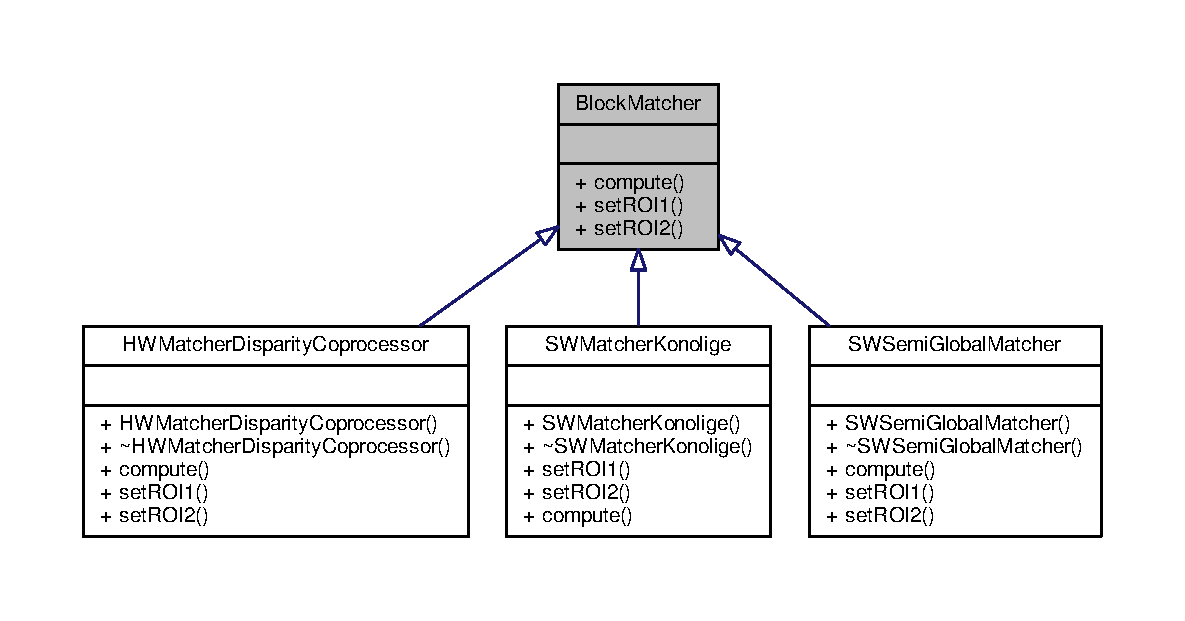
\includegraphics[width=350pt]{classBlockMatcher__inherit__graph}
\end{center}
\end{figure}


Collaboration diagram for Block\+Matcher\+:
\nopagebreak
\begin{figure}[H]
\begin{center}
\leavevmode
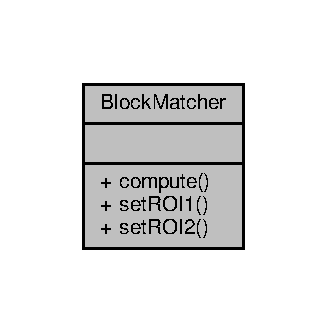
\includegraphics[width=157pt]{classBlockMatcher__coll__graph}
\end{center}
\end{figure}
\subsection*{Public Member Functions}
\begin{DoxyCompactItemize}
\item 
virtual int \hyperlink{classBlockMatcher_ae37e0c58790f4604f51549c518684c64}{compute} (cv\+::\+Input\+Array left, cv\+::\+Input\+Array right, cv\+::\+Output\+Array out)=0
\item 
virtual void \hyperlink{classBlockMatcher_a0b1c689296bea9085be223e53ba538a0}{set\+R\+O\+I1} (cv\+::\+Rect roi1)=0
\item 
virtual void \hyperlink{classBlockMatcher_af80a89fda1b2fd2d78e75e7466dcbcca}{set\+R\+O\+I2} (cv\+::\+Rect roi2)=0
\end{DoxyCompactItemize}


\subsection{Member Function Documentation}
\index{Block\+Matcher@{Block\+Matcher}!compute@{compute}}
\index{compute@{compute}!Block\+Matcher@{Block\+Matcher}}
\subsubsection[{\texorpdfstring{compute(cv\+::\+Input\+Array left, cv\+::\+Input\+Array right, cv\+::\+Output\+Array out)=0}{compute(cv::InputArray left, cv::InputArray right, cv::OutputArray out)=0}}]{\setlength{\rightskip}{0pt plus 5cm}virtual int Block\+Matcher\+::compute (
\begin{DoxyParamCaption}
\item[{cv\+::\+Input\+Array}]{left, }
\item[{cv\+::\+Input\+Array}]{right, }
\item[{cv\+::\+Output\+Array}]{out}
\end{DoxyParamCaption}
)\hspace{0.3cm}{\ttfamily [pure virtual]}}\hypertarget{classBlockMatcher_ae37e0c58790f4604f51549c518684c64}{}\label{classBlockMatcher_ae37e0c58790f4604f51549c518684c64}
\index{Block\+Matcher@{Block\+Matcher}!set\+R\+O\+I1@{set\+R\+O\+I1}}
\index{set\+R\+O\+I1@{set\+R\+O\+I1}!Block\+Matcher@{Block\+Matcher}}
\subsubsection[{\texorpdfstring{set\+R\+O\+I1(cv\+::\+Rect roi1)=0}{setROI1(cv::Rect roi1)=0}}]{\setlength{\rightskip}{0pt plus 5cm}virtual void Block\+Matcher\+::set\+R\+O\+I1 (
\begin{DoxyParamCaption}
\item[{cv\+::\+Rect}]{roi1}
\end{DoxyParamCaption}
)\hspace{0.3cm}{\ttfamily [pure virtual]}}\hypertarget{classBlockMatcher_a0b1c689296bea9085be223e53ba538a0}{}\label{classBlockMatcher_a0b1c689296bea9085be223e53ba538a0}


Implemented in \hyperlink{classHWMatcherDisparityCoprocessor_a3e267ddaad5c676e065c751d983efbf3}{H\+W\+Matcher\+Disparity\+Coprocessor}, \hyperlink{classSWMatcherKonolige_a70a376f1d07da7000ea0a88fc3ab673a}{S\+W\+Matcher\+Konolige}, and \hyperlink{classSWSemiGlobalMatcher_a67bf29294ea497441037616b1fb32769}{S\+W\+Semi\+Global\+Matcher}.

\index{Block\+Matcher@{Block\+Matcher}!set\+R\+O\+I2@{set\+R\+O\+I2}}
\index{set\+R\+O\+I2@{set\+R\+O\+I2}!Block\+Matcher@{Block\+Matcher}}
\subsubsection[{\texorpdfstring{set\+R\+O\+I2(cv\+::\+Rect roi2)=0}{setROI2(cv::Rect roi2)=0}}]{\setlength{\rightskip}{0pt plus 5cm}virtual void Block\+Matcher\+::set\+R\+O\+I2 (
\begin{DoxyParamCaption}
\item[{cv\+::\+Rect}]{roi2}
\end{DoxyParamCaption}
)\hspace{0.3cm}{\ttfamily [pure virtual]}}\hypertarget{classBlockMatcher_af80a89fda1b2fd2d78e75e7466dcbcca}{}\label{classBlockMatcher_af80a89fda1b2fd2d78e75e7466dcbcca}


Implemented in \hyperlink{classHWMatcherDisparityCoprocessor_af0eed2c0ada37722bbf7376369ace242}{H\+W\+Matcher\+Disparity\+Coprocessor}, \hyperlink{classSWMatcherKonolige_a05913005c4d1b5ea6b1bbcb79deef7d0}{S\+W\+Matcher\+Konolige}, and \hyperlink{classSWSemiGlobalMatcher_a8cfa467d703b6a38cbd9e3ff1f9a3f70}{S\+W\+Semi\+Global\+Matcher}.



The documentation for this class was generated from the following file\+:\begin{DoxyCompactItemize}
\item 
include/stereo-\/matcher/\hyperlink{stereo-matcher_8h}{stereo-\/matcher.\+h}\end{DoxyCompactItemize}

\hypertarget{structdcx__config}{}\section{dcx\+\_\+config Struct Reference}
\label{structdcx__config}\index{dcx\+\_\+config@{dcx\+\_\+config}}


{\ttfamily \#include $<$bm-\/hw-\/ip.\+h$>$}



Collaboration diagram for dcx\+\_\+config\+:
\nopagebreak
\begin{figure}[H]
\begin{center}
\leavevmode
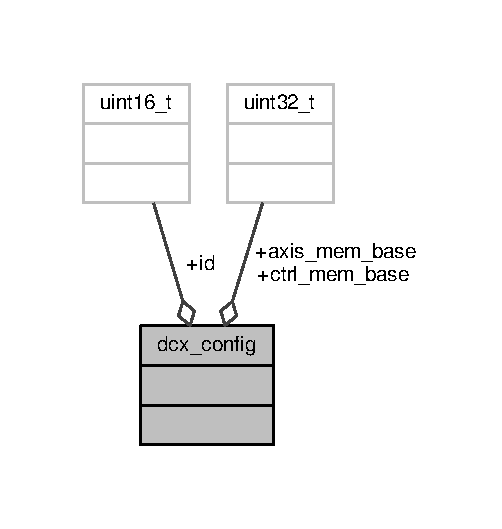
\includegraphics[width=241pt]{structdcx__config__coll__graph}
\end{center}
\end{figure}
\subsection*{Public Attributes}
\begin{DoxyCompactItemize}
\item 
uint16\+\_\+t \hyperlink{structdcx__config_a70e359a93971135101d7035d39eeca17}{id}
\item 
uint32\+\_\+t \hyperlink{structdcx__config_a75f8a6e408ba2b7a6f68c2171c2107d4}{ctrl\+\_\+mem\+\_\+base}
\item 
uint32\+\_\+t \hyperlink{structdcx__config_a9297308ad57eee72697c41660ccb2b86}{axis\+\_\+mem\+\_\+base}
\end{DoxyCompactItemize}


\subsection{Member Data Documentation}
\index{dcx\+\_\+config@{dcx\+\_\+config}!axis\+\_\+mem\+\_\+base@{axis\+\_\+mem\+\_\+base}}
\index{axis\+\_\+mem\+\_\+base@{axis\+\_\+mem\+\_\+base}!dcx\+\_\+config@{dcx\+\_\+config}}
\subsubsection[{\texorpdfstring{axis\+\_\+mem\+\_\+base}{axis_mem_base}}]{\setlength{\rightskip}{0pt plus 5cm}uint32\+\_\+t dcx\+\_\+config\+::axis\+\_\+mem\+\_\+base}\hypertarget{structdcx__config_a9297308ad57eee72697c41660ccb2b86}{}\label{structdcx__config_a9297308ad57eee72697c41660ccb2b86}
\index{dcx\+\_\+config@{dcx\+\_\+config}!ctrl\+\_\+mem\+\_\+base@{ctrl\+\_\+mem\+\_\+base}}
\index{ctrl\+\_\+mem\+\_\+base@{ctrl\+\_\+mem\+\_\+base}!dcx\+\_\+config@{dcx\+\_\+config}}
\subsubsection[{\texorpdfstring{ctrl\+\_\+mem\+\_\+base}{ctrl_mem_base}}]{\setlength{\rightskip}{0pt plus 5cm}uint32\+\_\+t dcx\+\_\+config\+::ctrl\+\_\+mem\+\_\+base}\hypertarget{structdcx__config_a75f8a6e408ba2b7a6f68c2171c2107d4}{}\label{structdcx__config_a75f8a6e408ba2b7a6f68c2171c2107d4}
\index{dcx\+\_\+config@{dcx\+\_\+config}!id@{id}}
\index{id@{id}!dcx\+\_\+config@{dcx\+\_\+config}}
\subsubsection[{\texorpdfstring{id}{id}}]{\setlength{\rightskip}{0pt plus 5cm}uint16\+\_\+t dcx\+\_\+config\+::id}\hypertarget{structdcx__config_a70e359a93971135101d7035d39eeca17}{}\label{structdcx__config_a70e359a93971135101d7035d39eeca17}


The documentation for this struct was generated from the following file\+:\begin{DoxyCompactItemize}
\item 
include/stereo-\/matcher/\hyperlink{bm-hw-ip_8h}{bm-\/hw-\/ip.\+h}\end{DoxyCompactItemize}

\hypertarget{structdcx__device}{}\section{dcx\+\_\+device Struct Reference}
\label{structdcx__device}\index{dcx\+\_\+device@{dcx\+\_\+device}}


{\ttfamily \#include $<$bm-\/hw-\/ip.\+h$>$}



Collaboration diagram for dcx\+\_\+device\+:
\nopagebreak
\begin{figure}[H]
\begin{center}
\leavevmode
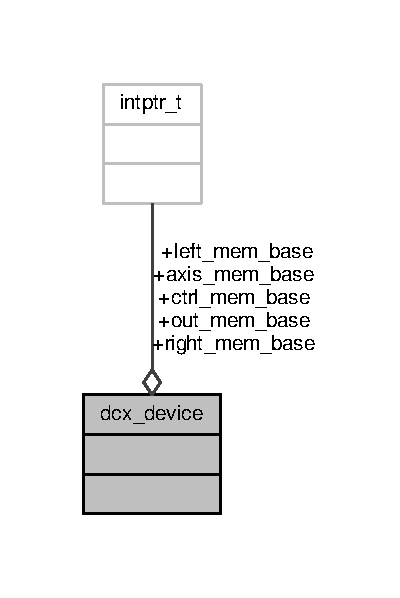
\includegraphics[width=192pt]{structdcx__device__coll__graph}
\end{center}
\end{figure}
\subsection*{Public Attributes}
\begin{DoxyCompactItemize}
\item 
intptr\+\_\+t \hyperlink{structdcx__device_a3564f065dedea6d4f215494e5549e394}{ctrl\+\_\+mem\+\_\+base}
\item 
intptr\+\_\+t \hyperlink{structdcx__device_a8de2b1be5c945cdffefb71048c430a52}{axis\+\_\+mem\+\_\+base}
\item 
intptr\+\_\+t \hyperlink{structdcx__device_aed5c8d74ac51c66da80b13c85e143b90}{left\+\_\+mem\+\_\+base}
\item 
intptr\+\_\+t \hyperlink{structdcx__device_a2878b0cea2e70a7a7d7299baa8f41d74}{right\+\_\+mem\+\_\+base}
\item 
intptr\+\_\+t \hyperlink{structdcx__device_a79059bdde1dae2b52111e4c0c723c356}{out\+\_\+mem\+\_\+base}
\end{DoxyCompactItemize}


\subsection{Member Data Documentation}
\index{dcx\+\_\+device@{dcx\+\_\+device}!axis\+\_\+mem\+\_\+base@{axis\+\_\+mem\+\_\+base}}
\index{axis\+\_\+mem\+\_\+base@{axis\+\_\+mem\+\_\+base}!dcx\+\_\+device@{dcx\+\_\+device}}
\subsubsection[{\texorpdfstring{axis\+\_\+mem\+\_\+base}{axis_mem_base}}]{\setlength{\rightskip}{0pt plus 5cm}intptr\+\_\+t dcx\+\_\+device\+::axis\+\_\+mem\+\_\+base}\hypertarget{structdcx__device_a8de2b1be5c945cdffefb71048c430a52}{}\label{structdcx__device_a8de2b1be5c945cdffefb71048c430a52}
\index{dcx\+\_\+device@{dcx\+\_\+device}!ctrl\+\_\+mem\+\_\+base@{ctrl\+\_\+mem\+\_\+base}}
\index{ctrl\+\_\+mem\+\_\+base@{ctrl\+\_\+mem\+\_\+base}!dcx\+\_\+device@{dcx\+\_\+device}}
\subsubsection[{\texorpdfstring{ctrl\+\_\+mem\+\_\+base}{ctrl_mem_base}}]{\setlength{\rightskip}{0pt plus 5cm}intptr\+\_\+t dcx\+\_\+device\+::ctrl\+\_\+mem\+\_\+base}\hypertarget{structdcx__device_a3564f065dedea6d4f215494e5549e394}{}\label{structdcx__device_a3564f065dedea6d4f215494e5549e394}
\index{dcx\+\_\+device@{dcx\+\_\+device}!left\+\_\+mem\+\_\+base@{left\+\_\+mem\+\_\+base}}
\index{left\+\_\+mem\+\_\+base@{left\+\_\+mem\+\_\+base}!dcx\+\_\+device@{dcx\+\_\+device}}
\subsubsection[{\texorpdfstring{left\+\_\+mem\+\_\+base}{left_mem_base}}]{\setlength{\rightskip}{0pt plus 5cm}intptr\+\_\+t dcx\+\_\+device\+::left\+\_\+mem\+\_\+base}\hypertarget{structdcx__device_aed5c8d74ac51c66da80b13c85e143b90}{}\label{structdcx__device_aed5c8d74ac51c66da80b13c85e143b90}
\index{dcx\+\_\+device@{dcx\+\_\+device}!out\+\_\+mem\+\_\+base@{out\+\_\+mem\+\_\+base}}
\index{out\+\_\+mem\+\_\+base@{out\+\_\+mem\+\_\+base}!dcx\+\_\+device@{dcx\+\_\+device}}
\subsubsection[{\texorpdfstring{out\+\_\+mem\+\_\+base}{out_mem_base}}]{\setlength{\rightskip}{0pt plus 5cm}intptr\+\_\+t dcx\+\_\+device\+::out\+\_\+mem\+\_\+base}\hypertarget{structdcx__device_a79059bdde1dae2b52111e4c0c723c356}{}\label{structdcx__device_a79059bdde1dae2b52111e4c0c723c356}
\index{dcx\+\_\+device@{dcx\+\_\+device}!right\+\_\+mem\+\_\+base@{right\+\_\+mem\+\_\+base}}
\index{right\+\_\+mem\+\_\+base@{right\+\_\+mem\+\_\+base}!dcx\+\_\+device@{dcx\+\_\+device}}
\subsubsection[{\texorpdfstring{right\+\_\+mem\+\_\+base}{right_mem_base}}]{\setlength{\rightskip}{0pt plus 5cm}intptr\+\_\+t dcx\+\_\+device\+::right\+\_\+mem\+\_\+base}\hypertarget{structdcx__device_a2878b0cea2e70a7a7d7299baa8f41d74}{}\label{structdcx__device_a2878b0cea2e70a7a7d7299baa8f41d74}


The documentation for this struct was generated from the following file\+:\begin{DoxyCompactItemize}
\item 
include/stereo-\/matcher/\hyperlink{bm-hw-ip_8h}{bm-\/hw-\/ip.\+h}\end{DoxyCompactItemize}

\hypertarget{structdcx__uio__info}{}\section{dcx\+\_\+uio\+\_\+info Struct Reference}
\label{structdcx__uio__info}\index{dcx\+\_\+uio\+\_\+info@{dcx\+\_\+uio\+\_\+info}}


{\ttfamily \#include $<$bm-\/hw-\/ip.\+h$>$}



Collaboration diagram for dcx\+\_\+uio\+\_\+info\+:
\nopagebreak
\begin{figure}[H]
\begin{center}
\leavevmode
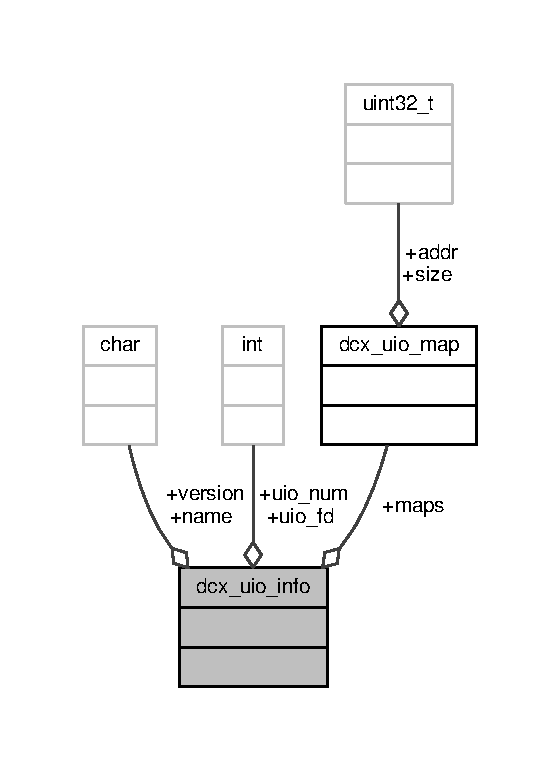
\includegraphics[width=269pt]{structdcx__uio__info__coll__graph}
\end{center}
\end{figure}
\subsection*{Public Attributes}
\begin{DoxyCompactItemize}
\item 
int \hyperlink{structdcx__uio__info_a2ebe1bdd70d7c34232ea3f85c1d591d3}{uio\+\_\+fd}
\item 
int \hyperlink{structdcx__uio__info_a02e1b0caf53d192f1d50de34f63d55a0}{uio\+\_\+num}
\item 
char \hyperlink{structdcx__uio__info_ab4b1a749035222b5f3ef16038284595f}{name} \mbox{[}\hyperlink{uio_8h_a5ed3f1c67d5551770a91ef53fe208c83}{M\+A\+X\+\_\+\+U\+I\+O\+\_\+\+N\+A\+M\+E\+\_\+\+S\+I\+ZE}\mbox{]}
\item 
char \hyperlink{structdcx__uio__info_ae1be148e26467d078ca0383c16f76a41}{version} \mbox{[}\hyperlink{uio_8h_a5ed3f1c67d5551770a91ef53fe208c83}{M\+A\+X\+\_\+\+U\+I\+O\+\_\+\+N\+A\+M\+E\+\_\+\+S\+I\+ZE}\mbox{]}
\item 
struct \hyperlink{structdcx__uio__map}{dcx\+\_\+uio\+\_\+map} \hyperlink{structdcx__uio__info_ae6e32e304b1afe3b2dfeeb1a54321919}{maps} \mbox{[}\hyperlink{uio_8h_a05a77cb47b9d8cdaaee64df37627ffdc}{M\+A\+X\+\_\+\+U\+I\+O\+\_\+\+M\+A\+PS}\mbox{]}
\end{DoxyCompactItemize}


\subsection{Member Data Documentation}
\index{dcx\+\_\+uio\+\_\+info@{dcx\+\_\+uio\+\_\+info}!maps@{maps}}
\index{maps@{maps}!dcx\+\_\+uio\+\_\+info@{dcx\+\_\+uio\+\_\+info}}
\subsubsection[{\texorpdfstring{maps}{maps}}]{\setlength{\rightskip}{0pt plus 5cm}struct {\bf dcx\+\_\+uio\+\_\+map} dcx\+\_\+uio\+\_\+info\+::maps\mbox{[}{\bf M\+A\+X\+\_\+\+U\+I\+O\+\_\+\+M\+A\+PS}\mbox{]}}\hypertarget{structdcx__uio__info_ae6e32e304b1afe3b2dfeeb1a54321919}{}\label{structdcx__uio__info_ae6e32e304b1afe3b2dfeeb1a54321919}
\index{dcx\+\_\+uio\+\_\+info@{dcx\+\_\+uio\+\_\+info}!name@{name}}
\index{name@{name}!dcx\+\_\+uio\+\_\+info@{dcx\+\_\+uio\+\_\+info}}
\subsubsection[{\texorpdfstring{name}{name}}]{\setlength{\rightskip}{0pt plus 5cm}char dcx\+\_\+uio\+\_\+info\+::name\mbox{[}{\bf M\+A\+X\+\_\+\+U\+I\+O\+\_\+\+N\+A\+M\+E\+\_\+\+S\+I\+ZE}\mbox{]}}\hypertarget{structdcx__uio__info_ab4b1a749035222b5f3ef16038284595f}{}\label{structdcx__uio__info_ab4b1a749035222b5f3ef16038284595f}
\index{dcx\+\_\+uio\+\_\+info@{dcx\+\_\+uio\+\_\+info}!uio\+\_\+fd@{uio\+\_\+fd}}
\index{uio\+\_\+fd@{uio\+\_\+fd}!dcx\+\_\+uio\+\_\+info@{dcx\+\_\+uio\+\_\+info}}
\subsubsection[{\texorpdfstring{uio\+\_\+fd}{uio_fd}}]{\setlength{\rightskip}{0pt plus 5cm}int dcx\+\_\+uio\+\_\+info\+::uio\+\_\+fd}\hypertarget{structdcx__uio__info_a2ebe1bdd70d7c34232ea3f85c1d591d3}{}\label{structdcx__uio__info_a2ebe1bdd70d7c34232ea3f85c1d591d3}
\index{dcx\+\_\+uio\+\_\+info@{dcx\+\_\+uio\+\_\+info}!uio\+\_\+num@{uio\+\_\+num}}
\index{uio\+\_\+num@{uio\+\_\+num}!dcx\+\_\+uio\+\_\+info@{dcx\+\_\+uio\+\_\+info}}
\subsubsection[{\texorpdfstring{uio\+\_\+num}{uio_num}}]{\setlength{\rightskip}{0pt plus 5cm}int dcx\+\_\+uio\+\_\+info\+::uio\+\_\+num}\hypertarget{structdcx__uio__info_a02e1b0caf53d192f1d50de34f63d55a0}{}\label{structdcx__uio__info_a02e1b0caf53d192f1d50de34f63d55a0}
\index{dcx\+\_\+uio\+\_\+info@{dcx\+\_\+uio\+\_\+info}!version@{version}}
\index{version@{version}!dcx\+\_\+uio\+\_\+info@{dcx\+\_\+uio\+\_\+info}}
\subsubsection[{\texorpdfstring{version}{version}}]{\setlength{\rightskip}{0pt plus 5cm}char dcx\+\_\+uio\+\_\+info\+::version\mbox{[}{\bf M\+A\+X\+\_\+\+U\+I\+O\+\_\+\+N\+A\+M\+E\+\_\+\+S\+I\+ZE}\mbox{]}}\hypertarget{structdcx__uio__info_ae1be148e26467d078ca0383c16f76a41}{}\label{structdcx__uio__info_ae1be148e26467d078ca0383c16f76a41}


The documentation for this struct was generated from the following file\+:\begin{DoxyCompactItemize}
\item 
include/stereo-\/matcher/\hyperlink{bm-hw-ip_8h}{bm-\/hw-\/ip.\+h}\end{DoxyCompactItemize}

\hypertarget{structdcx__uio__map}{}\section{dcx\+\_\+uio\+\_\+map Struct Reference}
\label{structdcx__uio__map}\index{dcx\+\_\+uio\+\_\+map@{dcx\+\_\+uio\+\_\+map}}


{\ttfamily \#include $<$bm-\/hw-\/ip.\+h$>$}



Collaboration diagram for dcx\+\_\+uio\+\_\+map\+:
\nopagebreak
\begin{figure}[H]
\begin{center}
\leavevmode
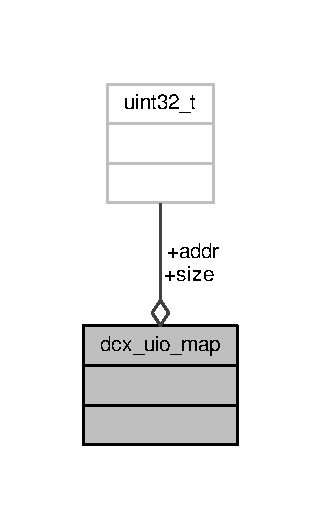
\includegraphics[width=154pt]{structdcx__uio__map__coll__graph}
\end{center}
\end{figure}
\subsection*{Public Attributes}
\begin{DoxyCompactItemize}
\item 
uint32\+\_\+t \hyperlink{structdcx__uio__map_a73ce78a039ea5795df6c831b8e011289}{addr}
\item 
uint32\+\_\+t \hyperlink{structdcx__uio__map_aa79438031223dcae6e71bebdc58ee8f3}{size}
\end{DoxyCompactItemize}


\subsection{Member Data Documentation}
\index{dcx\+\_\+uio\+\_\+map@{dcx\+\_\+uio\+\_\+map}!addr@{addr}}
\index{addr@{addr}!dcx\+\_\+uio\+\_\+map@{dcx\+\_\+uio\+\_\+map}}
\subsubsection[{\texorpdfstring{addr}{addr}}]{\setlength{\rightskip}{0pt plus 5cm}uint32\+\_\+t dcx\+\_\+uio\+\_\+map\+::addr}\hypertarget{structdcx__uio__map_a73ce78a039ea5795df6c831b8e011289}{}\label{structdcx__uio__map_a73ce78a039ea5795df6c831b8e011289}
\index{dcx\+\_\+uio\+\_\+map@{dcx\+\_\+uio\+\_\+map}!size@{size}}
\index{size@{size}!dcx\+\_\+uio\+\_\+map@{dcx\+\_\+uio\+\_\+map}}
\subsubsection[{\texorpdfstring{size}{size}}]{\setlength{\rightskip}{0pt plus 5cm}uint32\+\_\+t dcx\+\_\+uio\+\_\+map\+::size}\hypertarget{structdcx__uio__map_aa79438031223dcae6e71bebdc58ee8f3}{}\label{structdcx__uio__map_aa79438031223dcae6e71bebdc58ee8f3}


The documentation for this struct was generated from the following file\+:\begin{DoxyCompactItemize}
\item 
include/stereo-\/matcher/\hyperlink{bm-hw-ip_8h}{bm-\/hw-\/ip.\+h}\end{DoxyCompactItemize}

\hypertarget{classDecoderDevice}{}\section{Decoder\+Device Class Reference}
\label{classDecoderDevice}\index{Decoder\+Device@{Decoder\+Device}}


{\ttfamily \#include $<$decoder.\+h$>$}



Inheritance diagram for Decoder\+Device\+:
\nopagebreak
\begin{figure}[H]
\begin{center}
\leavevmode
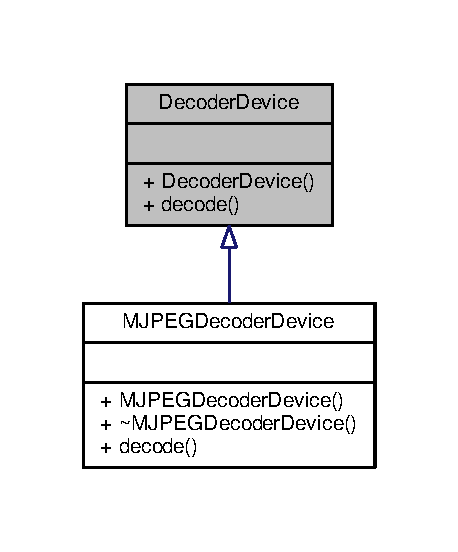
\includegraphics[width=220pt]{classDecoderDevice__inherit__graph}
\end{center}
\end{figure}


Collaboration diagram for Decoder\+Device\+:
\nopagebreak
\begin{figure}[H]
\begin{center}
\leavevmode
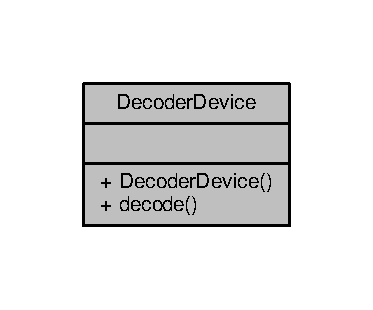
\includegraphics[width=179pt]{classDecoderDevice__coll__graph}
\end{center}
\end{figure}
\subsection*{Public Member Functions}
\begin{DoxyCompactItemize}
\item 
\hyperlink{classDecoderDevice_a2599f7d1eedfeb411d8d4e41f30d1934}{Decoder\+Device} ()
\item 
virtual int \hyperlink{classDecoderDevice_aadb33964bae3c6d9ad310105242d5611}{decode} (char $\ast$in, int len, int width, int height, char $\ast$out)=0
\end{DoxyCompactItemize}


\subsection{Constructor \& Destructor Documentation}
\index{Decoder\+Device@{Decoder\+Device}!Decoder\+Device@{Decoder\+Device}}
\index{Decoder\+Device@{Decoder\+Device}!Decoder\+Device@{Decoder\+Device}}
\subsubsection[{\texorpdfstring{Decoder\+Device()}{DecoderDevice()}}]{\setlength{\rightskip}{0pt plus 5cm}Decoder\+Device\+::\+Decoder\+Device (
\begin{DoxyParamCaption}
{}
\end{DoxyParamCaption}
)\hspace{0.3cm}{\ttfamily [explicit]}}\hypertarget{classDecoderDevice_a2599f7d1eedfeb411d8d4e41f30d1934}{}\label{classDecoderDevice_a2599f7d1eedfeb411d8d4e41f30d1934}


\subsection{Member Function Documentation}
\index{Decoder\+Device@{Decoder\+Device}!decode@{decode}}
\index{decode@{decode}!Decoder\+Device@{Decoder\+Device}}
\subsubsection[{\texorpdfstring{decode(char $\ast$in, int len, int width, int height, char $\ast$out)=0}{decode(char *in, int len, int width, int height, char *out)=0}}]{\setlength{\rightskip}{0pt plus 5cm}virtual int Decoder\+Device\+::decode (
\begin{DoxyParamCaption}
\item[{char $\ast$}]{in, }
\item[{int}]{len, }
\item[{int}]{width, }
\item[{int}]{height, }
\item[{char $\ast$}]{out}
\end{DoxyParamCaption}
)\hspace{0.3cm}{\ttfamily [pure virtual]}}\hypertarget{classDecoderDevice_aadb33964bae3c6d9ad310105242d5611}{}\label{classDecoderDevice_aadb33964bae3c6d9ad310105242d5611}


Implemented in \hyperlink{classMJPEGDecoderDevice_af765b926a83d573d5cf46a2c76d23597}{M\+J\+P\+E\+G\+Decoder\+Device}.



The documentation for this class was generated from the following files\+:\begin{DoxyCompactItemize}
\item 
include/decoder/\hyperlink{decoder_8h}{decoder.\+h}\item 
decoder/\hyperlink{decoder_8cpp}{decoder.\+cpp}\end{DoxyCompactItemize}

\hypertarget{structerror__mgr}{}\section{error\+\_\+mgr Struct Reference}
\label{structerror__mgr}\index{error\+\_\+mgr@{error\+\_\+mgr}}


Collaboration diagram for error\+\_\+mgr\+:
\nopagebreak
\begin{figure}[H]
\begin{center}
\leavevmode
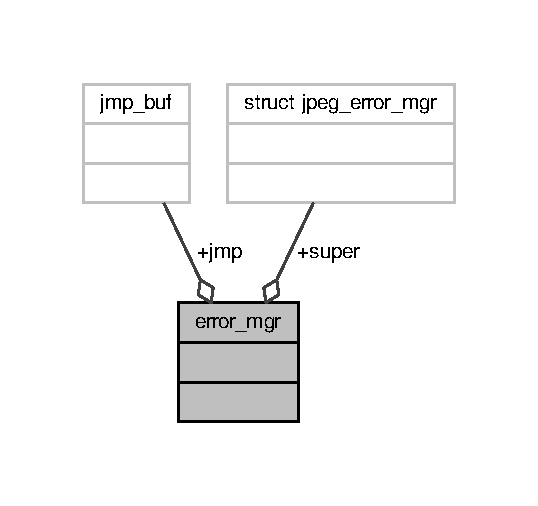
\includegraphics[width=258pt]{structerror__mgr__coll__graph}
\end{center}
\end{figure}
\subsection*{Public Attributes}
\begin{DoxyCompactItemize}
\item 
struct jpeg\+\_\+error\+\_\+mgr \hyperlink{structerror__mgr_a05d0382955eda152db1b6fa9ff3a3d6e}{super}
\item 
jmp\+\_\+buf \hyperlink{structerror__mgr_a1e0f88f95302e5df0a0a5ca8dac7ce9c}{jmp}
\end{DoxyCompactItemize}


\subsection{Member Data Documentation}
\index{error\+\_\+mgr@{error\+\_\+mgr}!jmp@{jmp}}
\index{jmp@{jmp}!error\+\_\+mgr@{error\+\_\+mgr}}
\subsubsection[{\texorpdfstring{jmp}{jmp}}]{\setlength{\rightskip}{0pt plus 5cm}jmp\+\_\+buf error\+\_\+mgr\+::jmp}\hypertarget{structerror__mgr_a1e0f88f95302e5df0a0a5ca8dac7ce9c}{}\label{structerror__mgr_a1e0f88f95302e5df0a0a5ca8dac7ce9c}
\index{error\+\_\+mgr@{error\+\_\+mgr}!super@{super}}
\index{super@{super}!error\+\_\+mgr@{error\+\_\+mgr}}
\subsubsection[{\texorpdfstring{super}{super}}]{\setlength{\rightskip}{0pt plus 5cm}struct jpeg\+\_\+error\+\_\+mgr error\+\_\+mgr\+::super}\hypertarget{structerror__mgr_a05d0382955eda152db1b6fa9ff3a3d6e}{}\label{structerror__mgr_a05d0382955eda152db1b6fa9ff3a3d6e}


The documentation for this struct was generated from the following file\+:\begin{DoxyCompactItemize}
\item 
decoder/\hyperlink{mjpeg-decoder-sw_8cpp}{mjpeg-\/decoder-\/sw.\+cpp}\end{DoxyCompactItemize}

\hypertarget{classEstimator}{}\section{Estimator Class Reference}
\label{classEstimator}\index{Estimator@{Estimator}}


{\ttfamily \#include $<$estimator.\+h$>$}



Collaboration diagram for Estimator\+:
\nopagebreak
\begin{figure}[H]
\begin{center}
\leavevmode
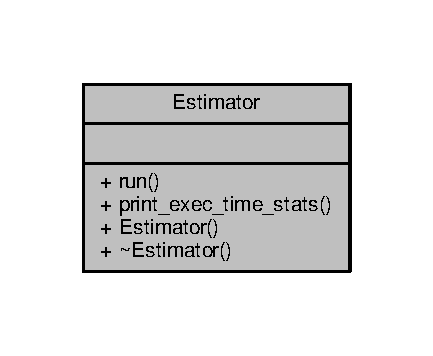
\includegraphics[width=208pt]{classEstimator__coll__graph}
\end{center}
\end{figure}
\subsection*{Public Member Functions}
\begin{DoxyCompactItemize}
\item 
void \hyperlink{classEstimator_a62e5a27e7c36023542faf730a14a7955}{run} ()
\item 
void \hyperlink{classEstimator_a2987abc6ac6b7978f681771a9b917c78}{print\+\_\+exec\+\_\+time\+\_\+stats} (void)
\item 
\hyperlink{classEstimator_a9dd72c43c2c708c7ea431f6d7aca7753}{Estimator} (\hyperlink{classBlockMatcher}{Block\+Matcher} $\ast$matcher, \hyperlink{classVideoFilterDevice}{Video\+Filter\+Device} $\ast$filter, \hyperlink{classVideoStreamStereoDevice}{Video\+Stream\+Stereo\+Device} $\ast$streamer, \hyperlink{classDecoderDevice}{Decoder\+Device} $\ast$decoder, \hyperlink{classEstimatorCmdLineParser}{Estimator\+Cmd\+Line\+Parser} $\ast$cmd\+Line\+Parser, Mat remap\+\_\+left1, Mat remap\+\_\+left2, Mat remap\+\_\+right1, Mat remap\+\_\+right2, Mat Q, Rect \&relevant\+Roi)
\item 
\hyperlink{classEstimator_a782584ccab2264d6c294ad7294150428}{$\sim$\+Estimator} ()
\end{DoxyCompactItemize}


\subsection{Constructor \& Destructor Documentation}
\index{Estimator@{Estimator}!Estimator@{Estimator}}
\index{Estimator@{Estimator}!Estimator@{Estimator}}
\subsubsection[{\texorpdfstring{Estimator(\+Block\+Matcher $\ast$matcher, Video\+Filter\+Device $\ast$filter, Video\+Stream\+Stereo\+Device $\ast$streamer, Decoder\+Device $\ast$decoder, Estimator\+Cmd\+Line\+Parser $\ast$cmd\+Line\+Parser, Mat remap\+\_\+left1, Mat remap\+\_\+left2, Mat remap\+\_\+right1, Mat remap\+\_\+right2, Mat Q, Rect \&relevant\+Roi)}{Estimator(BlockMatcher *matcher, VideoFilterDevice *filter, VideoStreamStereoDevice *streamer, DecoderDevice *decoder, EstimatorCmdLineParser *cmdLineParser, Mat remap_left1, Mat remap_left2, Mat remap_right1, Mat remap_right2, Mat Q, Rect &relevantRoi)}}]{\setlength{\rightskip}{0pt plus 5cm}Estimator\+::\+Estimator (
\begin{DoxyParamCaption}
\item[{{\bf Block\+Matcher} $\ast$}]{matcher, }
\item[{{\bf Video\+Filter\+Device} $\ast$}]{filter, }
\item[{{\bf Video\+Stream\+Stereo\+Device} $\ast$}]{streamer, }
\item[{{\bf Decoder\+Device} $\ast$}]{decoder, }
\item[{{\bf Estimator\+Cmd\+Line\+Parser} $\ast$}]{cmd\+Line\+Parser, }
\item[{Mat}]{remap\+\_\+left1, }
\item[{Mat}]{remap\+\_\+left2, }
\item[{Mat}]{remap\+\_\+right1, }
\item[{Mat}]{remap\+\_\+right2, }
\item[{Mat}]{Q, }
\item[{Rect \&}]{relevant\+Roi}
\end{DoxyParamCaption}
)}\hypertarget{classEstimator_a9dd72c43c2c708c7ea431f6d7aca7753}{}\label{classEstimator_a9dd72c43c2c708c7ea431f6d7aca7753}
\index{Estimator@{Estimator}!````~Estimator@{$\sim$\+Estimator}}
\index{````~Estimator@{$\sim$\+Estimator}!Estimator@{Estimator}}
\subsubsection[{\texorpdfstring{$\sim$\+Estimator()}{~Estimator()}}]{\setlength{\rightskip}{0pt plus 5cm}Estimator\+::$\sim$\+Estimator (
\begin{DoxyParamCaption}
{}
\end{DoxyParamCaption}
)}\hypertarget{classEstimator_a782584ccab2264d6c294ad7294150428}{}\label{classEstimator_a782584ccab2264d6c294ad7294150428}


\subsection{Member Function Documentation}
\index{Estimator@{Estimator}!print\+\_\+exec\+\_\+time\+\_\+stats@{print\+\_\+exec\+\_\+time\+\_\+stats}}
\index{print\+\_\+exec\+\_\+time\+\_\+stats@{print\+\_\+exec\+\_\+time\+\_\+stats}!Estimator@{Estimator}}
\subsubsection[{\texorpdfstring{print\+\_\+exec\+\_\+time\+\_\+stats(void)}{print_exec_time_stats(void)}}]{\setlength{\rightskip}{0pt plus 5cm}void Estimator\+::print\+\_\+exec\+\_\+time\+\_\+stats (
\begin{DoxyParamCaption}
\item[{void}]{}
\end{DoxyParamCaption}
)}\hypertarget{classEstimator_a2987abc6ac6b7978f681771a9b917c78}{}\label{classEstimator_a2987abc6ac6b7978f681771a9b917c78}
\index{Estimator@{Estimator}!run@{run}}
\index{run@{run}!Estimator@{Estimator}}
\subsubsection[{\texorpdfstring{run()}{run()}}]{\setlength{\rightskip}{0pt plus 5cm}void Estimator\+::run (
\begin{DoxyParamCaption}
{}
\end{DoxyParamCaption}
)}\hypertarget{classEstimator_a62e5a27e7c36023542faf730a14a7955}{}\label{classEstimator_a62e5a27e7c36023542faf730a14a7955}


The documentation for this class was generated from the following files\+:\begin{DoxyCompactItemize}
\item 
include/\hyperlink{estimator_8h}{estimator.\+h}\item 
\hyperlink{estimator_8cpp}{estimator.\+cpp}\end{DoxyCompactItemize}

\hypertarget{classEstimatorCmdLineParser}{}\section{Estimator\+Cmd\+Line\+Parser Class Reference}
\label{classEstimatorCmdLineParser}\index{Estimator\+Cmd\+Line\+Parser@{Estimator\+Cmd\+Line\+Parser}}


{\ttfamily \#include $<$cmdline-\/parser.\+h$>$}



Collaboration diagram for Estimator\+Cmd\+Line\+Parser\+:
\nopagebreak
\begin{figure}[H]
\begin{center}
\leavevmode
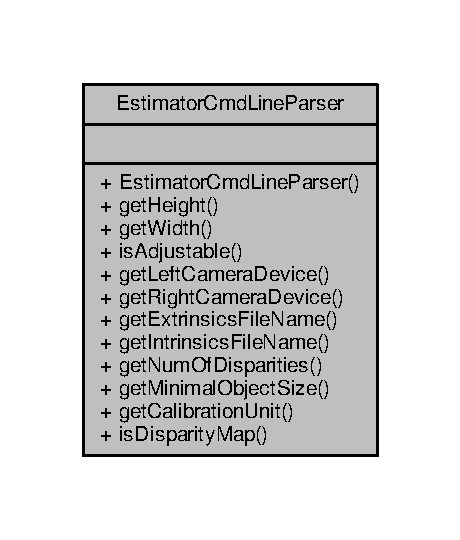
\includegraphics[width=221pt]{classEstimatorCmdLineParser__coll__graph}
\end{center}
\end{figure}
\subsection*{Public Member Functions}
\begin{DoxyCompactItemize}
\item 
\hyperlink{classEstimatorCmdLineParser_a63d7e43b228b8a91808d5a9d294866fd}{Estimator\+Cmd\+Line\+Parser} (char $\ast$$\ast$cmd\+\_\+options, int num\+\_\+options)
\item 
int \hyperlink{classEstimatorCmdLineParser_a20a512e1e58330dfb8f1ab72db990200}{get\+Height} () const 
\item 
int \hyperlink{classEstimatorCmdLineParser_ac41c01b0d7f2804842e6288e09d77182}{get\+Width} () const 
\item 
bool \hyperlink{classEstimatorCmdLineParser_a6cb61d5b5337cf23d4e35eb6b4ea2bcd}{is\+Adjustable} () const 
\item 
const String \& \hyperlink{classEstimatorCmdLineParser_a50d983eb935a86bd0834b35092a8669e}{get\+Left\+Camera\+Device} () const 
\item 
const String \& \hyperlink{classEstimatorCmdLineParser_a2ebbfb26a0a57f47003cd063b987f565}{get\+Right\+Camera\+Device} () const 
\item 
const String \& \hyperlink{classEstimatorCmdLineParser_aec4d9e6eef122e68689a3f3cf7405de8}{get\+Extrinsics\+File\+Name} () const 
\item 
const String \& \hyperlink{classEstimatorCmdLineParser_aa132b17af56498023d77d9b05313ff9f}{get\+Intrinsics\+File\+Name} () const 
\item 
int \hyperlink{classEstimatorCmdLineParser_a088ac9d1832dad1b27b0d6760837fd8f}{get\+Num\+Of\+Disparities} () const 
\item 
int \hyperlink{classEstimatorCmdLineParser_ad52089aede854ef22a402cc9d292c353}{get\+Minimal\+Object\+Size} () const 
\item 
double \hyperlink{classEstimatorCmdLineParser_a500dd919b026ea289aa4395d67e9259c}{get\+Calibration\+Unit} () const 
\item 
bool \hyperlink{classEstimatorCmdLineParser_aed638d37a28b85d2aa822b8cc58c11de}{is\+Disparity\+Map} () const 
\end{DoxyCompactItemize}


\subsection{Constructor \& Destructor Documentation}
\index{Estimator\+Cmd\+Line\+Parser@{Estimator\+Cmd\+Line\+Parser}!Estimator\+Cmd\+Line\+Parser@{Estimator\+Cmd\+Line\+Parser}}
\index{Estimator\+Cmd\+Line\+Parser@{Estimator\+Cmd\+Line\+Parser}!Estimator\+Cmd\+Line\+Parser@{Estimator\+Cmd\+Line\+Parser}}
\subsubsection[{\texorpdfstring{Estimator\+Cmd\+Line\+Parser(char $\ast$$\ast$cmd\+\_\+options, int num\+\_\+options)}{EstimatorCmdLineParser(char **cmd_options, int num_options)}}]{\setlength{\rightskip}{0pt plus 5cm}Estimator\+Cmd\+Line\+Parser\+::\+Estimator\+Cmd\+Line\+Parser (
\begin{DoxyParamCaption}
\item[{char $\ast$$\ast$}]{cmd\+\_\+options, }
\item[{int}]{num\+\_\+options}
\end{DoxyParamCaption}
)}\hypertarget{classEstimatorCmdLineParser_a63d7e43b228b8a91808d5a9d294866fd}{}\label{classEstimatorCmdLineParser_a63d7e43b228b8a91808d5a9d294866fd}


\subsection{Member Function Documentation}
\index{Estimator\+Cmd\+Line\+Parser@{Estimator\+Cmd\+Line\+Parser}!get\+Calibration\+Unit@{get\+Calibration\+Unit}}
\index{get\+Calibration\+Unit@{get\+Calibration\+Unit}!Estimator\+Cmd\+Line\+Parser@{Estimator\+Cmd\+Line\+Parser}}
\subsubsection[{\texorpdfstring{get\+Calibration\+Unit() const }{getCalibrationUnit() const }}]{\setlength{\rightskip}{0pt plus 5cm}double Estimator\+Cmd\+Line\+Parser\+::get\+Calibration\+Unit (
\begin{DoxyParamCaption}
{}
\end{DoxyParamCaption}
) const\hspace{0.3cm}{\ttfamily [inline]}}\hypertarget{classEstimatorCmdLineParser_a500dd919b026ea289aa4395d67e9259c}{}\label{classEstimatorCmdLineParser_a500dd919b026ea289aa4395d67e9259c}
\index{Estimator\+Cmd\+Line\+Parser@{Estimator\+Cmd\+Line\+Parser}!get\+Extrinsics\+File\+Name@{get\+Extrinsics\+File\+Name}}
\index{get\+Extrinsics\+File\+Name@{get\+Extrinsics\+File\+Name}!Estimator\+Cmd\+Line\+Parser@{Estimator\+Cmd\+Line\+Parser}}
\subsubsection[{\texorpdfstring{get\+Extrinsics\+File\+Name() const }{getExtrinsicsFileName() const }}]{\setlength{\rightskip}{0pt plus 5cm}const String\& Estimator\+Cmd\+Line\+Parser\+::get\+Extrinsics\+File\+Name (
\begin{DoxyParamCaption}
{}
\end{DoxyParamCaption}
) const\hspace{0.3cm}{\ttfamily [inline]}}\hypertarget{classEstimatorCmdLineParser_aec4d9e6eef122e68689a3f3cf7405de8}{}\label{classEstimatorCmdLineParser_aec4d9e6eef122e68689a3f3cf7405de8}
\index{Estimator\+Cmd\+Line\+Parser@{Estimator\+Cmd\+Line\+Parser}!get\+Height@{get\+Height}}
\index{get\+Height@{get\+Height}!Estimator\+Cmd\+Line\+Parser@{Estimator\+Cmd\+Line\+Parser}}
\subsubsection[{\texorpdfstring{get\+Height() const }{getHeight() const }}]{\setlength{\rightskip}{0pt plus 5cm}int Estimator\+Cmd\+Line\+Parser\+::get\+Height (
\begin{DoxyParamCaption}
{}
\end{DoxyParamCaption}
) const\hspace{0.3cm}{\ttfamily [inline]}}\hypertarget{classEstimatorCmdLineParser_a20a512e1e58330dfb8f1ab72db990200}{}\label{classEstimatorCmdLineParser_a20a512e1e58330dfb8f1ab72db990200}
\index{Estimator\+Cmd\+Line\+Parser@{Estimator\+Cmd\+Line\+Parser}!get\+Intrinsics\+File\+Name@{get\+Intrinsics\+File\+Name}}
\index{get\+Intrinsics\+File\+Name@{get\+Intrinsics\+File\+Name}!Estimator\+Cmd\+Line\+Parser@{Estimator\+Cmd\+Line\+Parser}}
\subsubsection[{\texorpdfstring{get\+Intrinsics\+File\+Name() const }{getIntrinsicsFileName() const }}]{\setlength{\rightskip}{0pt plus 5cm}const String\& Estimator\+Cmd\+Line\+Parser\+::get\+Intrinsics\+File\+Name (
\begin{DoxyParamCaption}
{}
\end{DoxyParamCaption}
) const\hspace{0.3cm}{\ttfamily [inline]}}\hypertarget{classEstimatorCmdLineParser_aa132b17af56498023d77d9b05313ff9f}{}\label{classEstimatorCmdLineParser_aa132b17af56498023d77d9b05313ff9f}
\index{Estimator\+Cmd\+Line\+Parser@{Estimator\+Cmd\+Line\+Parser}!get\+Left\+Camera\+Device@{get\+Left\+Camera\+Device}}
\index{get\+Left\+Camera\+Device@{get\+Left\+Camera\+Device}!Estimator\+Cmd\+Line\+Parser@{Estimator\+Cmd\+Line\+Parser}}
\subsubsection[{\texorpdfstring{get\+Left\+Camera\+Device() const }{getLeftCameraDevice() const }}]{\setlength{\rightskip}{0pt plus 5cm}const String\& Estimator\+Cmd\+Line\+Parser\+::get\+Left\+Camera\+Device (
\begin{DoxyParamCaption}
{}
\end{DoxyParamCaption}
) const\hspace{0.3cm}{\ttfamily [inline]}}\hypertarget{classEstimatorCmdLineParser_a50d983eb935a86bd0834b35092a8669e}{}\label{classEstimatorCmdLineParser_a50d983eb935a86bd0834b35092a8669e}
\index{Estimator\+Cmd\+Line\+Parser@{Estimator\+Cmd\+Line\+Parser}!get\+Minimal\+Object\+Size@{get\+Minimal\+Object\+Size}}
\index{get\+Minimal\+Object\+Size@{get\+Minimal\+Object\+Size}!Estimator\+Cmd\+Line\+Parser@{Estimator\+Cmd\+Line\+Parser}}
\subsubsection[{\texorpdfstring{get\+Minimal\+Object\+Size() const }{getMinimalObjectSize() const }}]{\setlength{\rightskip}{0pt plus 5cm}int Estimator\+Cmd\+Line\+Parser\+::get\+Minimal\+Object\+Size (
\begin{DoxyParamCaption}
{}
\end{DoxyParamCaption}
) const\hspace{0.3cm}{\ttfamily [inline]}}\hypertarget{classEstimatorCmdLineParser_ad52089aede854ef22a402cc9d292c353}{}\label{classEstimatorCmdLineParser_ad52089aede854ef22a402cc9d292c353}
\index{Estimator\+Cmd\+Line\+Parser@{Estimator\+Cmd\+Line\+Parser}!get\+Num\+Of\+Disparities@{get\+Num\+Of\+Disparities}}
\index{get\+Num\+Of\+Disparities@{get\+Num\+Of\+Disparities}!Estimator\+Cmd\+Line\+Parser@{Estimator\+Cmd\+Line\+Parser}}
\subsubsection[{\texorpdfstring{get\+Num\+Of\+Disparities() const }{getNumOfDisparities() const }}]{\setlength{\rightskip}{0pt plus 5cm}int Estimator\+Cmd\+Line\+Parser\+::get\+Num\+Of\+Disparities (
\begin{DoxyParamCaption}
{}
\end{DoxyParamCaption}
) const\hspace{0.3cm}{\ttfamily [inline]}}\hypertarget{classEstimatorCmdLineParser_a088ac9d1832dad1b27b0d6760837fd8f}{}\label{classEstimatorCmdLineParser_a088ac9d1832dad1b27b0d6760837fd8f}
\index{Estimator\+Cmd\+Line\+Parser@{Estimator\+Cmd\+Line\+Parser}!get\+Right\+Camera\+Device@{get\+Right\+Camera\+Device}}
\index{get\+Right\+Camera\+Device@{get\+Right\+Camera\+Device}!Estimator\+Cmd\+Line\+Parser@{Estimator\+Cmd\+Line\+Parser}}
\subsubsection[{\texorpdfstring{get\+Right\+Camera\+Device() const }{getRightCameraDevice() const }}]{\setlength{\rightskip}{0pt plus 5cm}const String\& Estimator\+Cmd\+Line\+Parser\+::get\+Right\+Camera\+Device (
\begin{DoxyParamCaption}
{}
\end{DoxyParamCaption}
) const\hspace{0.3cm}{\ttfamily [inline]}}\hypertarget{classEstimatorCmdLineParser_a2ebbfb26a0a57f47003cd063b987f565}{}\label{classEstimatorCmdLineParser_a2ebbfb26a0a57f47003cd063b987f565}
\index{Estimator\+Cmd\+Line\+Parser@{Estimator\+Cmd\+Line\+Parser}!get\+Width@{get\+Width}}
\index{get\+Width@{get\+Width}!Estimator\+Cmd\+Line\+Parser@{Estimator\+Cmd\+Line\+Parser}}
\subsubsection[{\texorpdfstring{get\+Width() const }{getWidth() const }}]{\setlength{\rightskip}{0pt plus 5cm}int Estimator\+Cmd\+Line\+Parser\+::get\+Width (
\begin{DoxyParamCaption}
{}
\end{DoxyParamCaption}
) const\hspace{0.3cm}{\ttfamily [inline]}}\hypertarget{classEstimatorCmdLineParser_ac41c01b0d7f2804842e6288e09d77182}{}\label{classEstimatorCmdLineParser_ac41c01b0d7f2804842e6288e09d77182}
\index{Estimator\+Cmd\+Line\+Parser@{Estimator\+Cmd\+Line\+Parser}!is\+Adjustable@{is\+Adjustable}}
\index{is\+Adjustable@{is\+Adjustable}!Estimator\+Cmd\+Line\+Parser@{Estimator\+Cmd\+Line\+Parser}}
\subsubsection[{\texorpdfstring{is\+Adjustable() const }{isAdjustable() const }}]{\setlength{\rightskip}{0pt plus 5cm}bool Estimator\+Cmd\+Line\+Parser\+::is\+Adjustable (
\begin{DoxyParamCaption}
{}
\end{DoxyParamCaption}
) const\hspace{0.3cm}{\ttfamily [inline]}}\hypertarget{classEstimatorCmdLineParser_a6cb61d5b5337cf23d4e35eb6b4ea2bcd}{}\label{classEstimatorCmdLineParser_a6cb61d5b5337cf23d4e35eb6b4ea2bcd}
\index{Estimator\+Cmd\+Line\+Parser@{Estimator\+Cmd\+Line\+Parser}!is\+Disparity\+Map@{is\+Disparity\+Map}}
\index{is\+Disparity\+Map@{is\+Disparity\+Map}!Estimator\+Cmd\+Line\+Parser@{Estimator\+Cmd\+Line\+Parser}}
\subsubsection[{\texorpdfstring{is\+Disparity\+Map() const }{isDisparityMap() const }}]{\setlength{\rightskip}{0pt plus 5cm}bool Estimator\+Cmd\+Line\+Parser\+::is\+Disparity\+Map (
\begin{DoxyParamCaption}
{}
\end{DoxyParamCaption}
) const\hspace{0.3cm}{\ttfamily [inline]}}\hypertarget{classEstimatorCmdLineParser_aed638d37a28b85d2aa822b8cc58c11de}{}\label{classEstimatorCmdLineParser_aed638d37a28b85d2aa822b8cc58c11de}


The documentation for this class was generated from the following files\+:\begin{DoxyCompactItemize}
\item 
include/utils/\hyperlink{cmdline-parser_8h}{cmdline-\/parser.\+h}\item 
utils/\hyperlink{cmdline-parser_8cpp}{cmdline-\/parser.\+cpp}\end{DoxyCompactItemize}

\hypertarget{structexec__time__struct}{}\section{exec\+\_\+time\+\_\+struct Struct Reference}
\label{structexec__time__struct}\index{exec\+\_\+time\+\_\+struct@{exec\+\_\+time\+\_\+struct}}


{\ttfamily \#include $<$estimator.\+h$>$}



Collaboration diagram for exec\+\_\+time\+\_\+struct\+:
\nopagebreak
\begin{figure}[H]
\begin{center}
\leavevmode
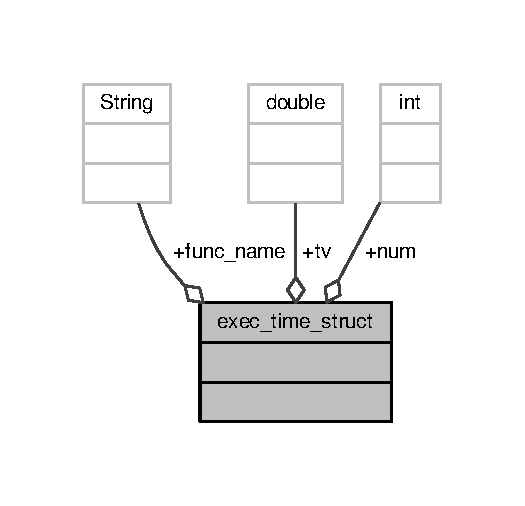
\includegraphics[width=252pt]{structexec__time__struct__coll__graph}
\end{center}
\end{figure}
\subsection*{Public Attributes}
\begin{DoxyCompactItemize}
\item 
String \hyperlink{structexec__time__struct_a29e6eb640031d9511b93e6f804ce5378}{func\+\_\+name}
\item 
double \hyperlink{structexec__time__struct_a58e8eec3a309584d7e9dfc76b1a38f62}{tv}
\item 
int \hyperlink{structexec__time__struct_ae25487e7ece38060f921344945dae62d}{num}
\end{DoxyCompactItemize}


\subsection{Member Data Documentation}
\index{exec\+\_\+time\+\_\+struct@{exec\+\_\+time\+\_\+struct}!func\+\_\+name@{func\+\_\+name}}
\index{func\+\_\+name@{func\+\_\+name}!exec\+\_\+time\+\_\+struct@{exec\+\_\+time\+\_\+struct}}
\subsubsection[{\texorpdfstring{func\+\_\+name}{func_name}}]{\setlength{\rightskip}{0pt plus 5cm}String exec\+\_\+time\+\_\+struct\+::func\+\_\+name}\hypertarget{structexec__time__struct_a29e6eb640031d9511b93e6f804ce5378}{}\label{structexec__time__struct_a29e6eb640031d9511b93e6f804ce5378}
\index{exec\+\_\+time\+\_\+struct@{exec\+\_\+time\+\_\+struct}!num@{num}}
\index{num@{num}!exec\+\_\+time\+\_\+struct@{exec\+\_\+time\+\_\+struct}}
\subsubsection[{\texorpdfstring{num}{num}}]{\setlength{\rightskip}{0pt plus 5cm}int exec\+\_\+time\+\_\+struct\+::num}\hypertarget{structexec__time__struct_ae25487e7ece38060f921344945dae62d}{}\label{structexec__time__struct_ae25487e7ece38060f921344945dae62d}
\index{exec\+\_\+time\+\_\+struct@{exec\+\_\+time\+\_\+struct}!tv@{tv}}
\index{tv@{tv}!exec\+\_\+time\+\_\+struct@{exec\+\_\+time\+\_\+struct}}
\subsubsection[{\texorpdfstring{tv}{tv}}]{\setlength{\rightskip}{0pt plus 5cm}double exec\+\_\+time\+\_\+struct\+::tv}\hypertarget{structexec__time__struct_a58e8eec3a309584d7e9dfc76b1a38f62}{}\label{structexec__time__struct_a58e8eec3a309584d7e9dfc76b1a38f62}


The documentation for this struct was generated from the following file\+:\begin{DoxyCompactItemize}
\item 
include/\hyperlink{estimator_8h}{estimator.\+h}\end{DoxyCompactItemize}

\hypertarget{structhsv__object__ranges}{}\section{hsv\+\_\+object\+\_\+ranges Struct Reference}
\label{structhsv__object__ranges}\index{hsv\+\_\+object\+\_\+ranges@{hsv\+\_\+object\+\_\+ranges}}


Collaboration diagram for hsv\+\_\+object\+\_\+ranges\+:
\nopagebreak
\begin{figure}[H]
\begin{center}
\leavevmode
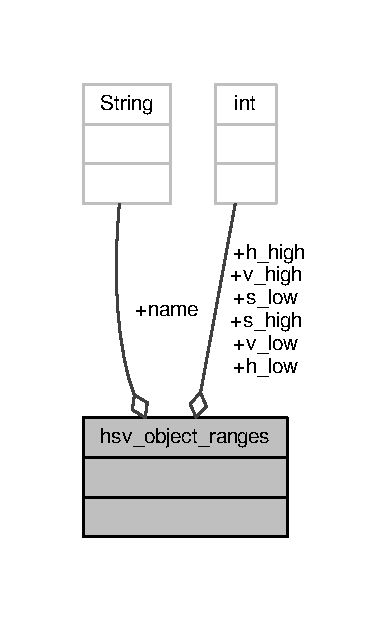
\includegraphics[width=187pt]{structhsv__object__ranges__coll__graph}
\end{center}
\end{figure}
\subsection*{Public Attributes}
\begin{DoxyCompactItemize}
\item 
String \hyperlink{structhsv__object__ranges_a087e260cfb50d9490ad05633d11ded77}{name}
\item 
int \hyperlink{structhsv__object__ranges_a362302fe5abaf418c33c49639093974f}{h\+\_\+low}
\item 
int \hyperlink{structhsv__object__ranges_aa38c3a60afec73cadef5fa88dc839f0d}{h\+\_\+high}
\item 
int \hyperlink{structhsv__object__ranges_a88708aeb732887c5b8e2b5c0809de85c}{s\+\_\+low}
\item 
int \hyperlink{structhsv__object__ranges_ab49c867dfdfbcf720be3b75e2379f093}{s\+\_\+high}
\item 
int \hyperlink{structhsv__object__ranges_a2e1235a8053f3bd1ae5b1b183bd7ab8f}{v\+\_\+low}
\item 
int \hyperlink{structhsv__object__ranges_a00ca3df99b0bdeac1cb7157fc0e3fbf7}{v\+\_\+high}
\end{DoxyCompactItemize}


\subsection{Member Data Documentation}
\index{hsv\+\_\+object\+\_\+ranges@{hsv\+\_\+object\+\_\+ranges}!h\+\_\+high@{h\+\_\+high}}
\index{h\+\_\+high@{h\+\_\+high}!hsv\+\_\+object\+\_\+ranges@{hsv\+\_\+object\+\_\+ranges}}
\subsubsection[{\texorpdfstring{h\+\_\+high}{h_high}}]{\setlength{\rightskip}{0pt plus 5cm}int hsv\+\_\+object\+\_\+ranges\+::h\+\_\+high}\hypertarget{structhsv__object__ranges_aa38c3a60afec73cadef5fa88dc839f0d}{}\label{structhsv__object__ranges_aa38c3a60afec73cadef5fa88dc839f0d}
\index{hsv\+\_\+object\+\_\+ranges@{hsv\+\_\+object\+\_\+ranges}!h\+\_\+low@{h\+\_\+low}}
\index{h\+\_\+low@{h\+\_\+low}!hsv\+\_\+object\+\_\+ranges@{hsv\+\_\+object\+\_\+ranges}}
\subsubsection[{\texorpdfstring{h\+\_\+low}{h_low}}]{\setlength{\rightskip}{0pt plus 5cm}int hsv\+\_\+object\+\_\+ranges\+::h\+\_\+low}\hypertarget{structhsv__object__ranges_a362302fe5abaf418c33c49639093974f}{}\label{structhsv__object__ranges_a362302fe5abaf418c33c49639093974f}
\index{hsv\+\_\+object\+\_\+ranges@{hsv\+\_\+object\+\_\+ranges}!name@{name}}
\index{name@{name}!hsv\+\_\+object\+\_\+ranges@{hsv\+\_\+object\+\_\+ranges}}
\subsubsection[{\texorpdfstring{name}{name}}]{\setlength{\rightskip}{0pt plus 5cm}String hsv\+\_\+object\+\_\+ranges\+::name}\hypertarget{structhsv__object__ranges_a087e260cfb50d9490ad05633d11ded77}{}\label{structhsv__object__ranges_a087e260cfb50d9490ad05633d11ded77}
\index{hsv\+\_\+object\+\_\+ranges@{hsv\+\_\+object\+\_\+ranges}!s\+\_\+high@{s\+\_\+high}}
\index{s\+\_\+high@{s\+\_\+high}!hsv\+\_\+object\+\_\+ranges@{hsv\+\_\+object\+\_\+ranges}}
\subsubsection[{\texorpdfstring{s\+\_\+high}{s_high}}]{\setlength{\rightskip}{0pt plus 5cm}int hsv\+\_\+object\+\_\+ranges\+::s\+\_\+high}\hypertarget{structhsv__object__ranges_ab49c867dfdfbcf720be3b75e2379f093}{}\label{structhsv__object__ranges_ab49c867dfdfbcf720be3b75e2379f093}
\index{hsv\+\_\+object\+\_\+ranges@{hsv\+\_\+object\+\_\+ranges}!s\+\_\+low@{s\+\_\+low}}
\index{s\+\_\+low@{s\+\_\+low}!hsv\+\_\+object\+\_\+ranges@{hsv\+\_\+object\+\_\+ranges}}
\subsubsection[{\texorpdfstring{s\+\_\+low}{s_low}}]{\setlength{\rightskip}{0pt plus 5cm}int hsv\+\_\+object\+\_\+ranges\+::s\+\_\+low}\hypertarget{structhsv__object__ranges_a88708aeb732887c5b8e2b5c0809de85c}{}\label{structhsv__object__ranges_a88708aeb732887c5b8e2b5c0809de85c}
\index{hsv\+\_\+object\+\_\+ranges@{hsv\+\_\+object\+\_\+ranges}!v\+\_\+high@{v\+\_\+high}}
\index{v\+\_\+high@{v\+\_\+high}!hsv\+\_\+object\+\_\+ranges@{hsv\+\_\+object\+\_\+ranges}}
\subsubsection[{\texorpdfstring{v\+\_\+high}{v_high}}]{\setlength{\rightskip}{0pt plus 5cm}int hsv\+\_\+object\+\_\+ranges\+::v\+\_\+high}\hypertarget{structhsv__object__ranges_a00ca3df99b0bdeac1cb7157fc0e3fbf7}{}\label{structhsv__object__ranges_a00ca3df99b0bdeac1cb7157fc0e3fbf7}
\index{hsv\+\_\+object\+\_\+ranges@{hsv\+\_\+object\+\_\+ranges}!v\+\_\+low@{v\+\_\+low}}
\index{v\+\_\+low@{v\+\_\+low}!hsv\+\_\+object\+\_\+ranges@{hsv\+\_\+object\+\_\+ranges}}
\subsubsection[{\texorpdfstring{v\+\_\+low}{v_low}}]{\setlength{\rightskip}{0pt plus 5cm}int hsv\+\_\+object\+\_\+ranges\+::v\+\_\+low}\hypertarget{structhsv__object__ranges_a2e1235a8053f3bd1ae5b1b183bd7ab8f}{}\label{structhsv__object__ranges_a2e1235a8053f3bd1ae5b1b183bd7ab8f}


The documentation for this struct was generated from the following file\+:\begin{DoxyCompactItemize}
\item 
\hyperlink{main_8cpp}{main.\+cpp}\end{DoxyCompactItemize}

\hypertarget{classHWMatcherDisparityCoprocessor}{}\section{H\+W\+Matcher\+Disparity\+Coprocessor Class Reference}
\label{classHWMatcherDisparityCoprocessor}\index{H\+W\+Matcher\+Disparity\+Coprocessor@{H\+W\+Matcher\+Disparity\+Coprocessor}}


{\ttfamily \#include $<$bm-\/hw-\/ip.\+h$>$}



Inheritance diagram for H\+W\+Matcher\+Disparity\+Coprocessor\+:
\nopagebreak
\begin{figure}[H]
\begin{center}
\leavevmode
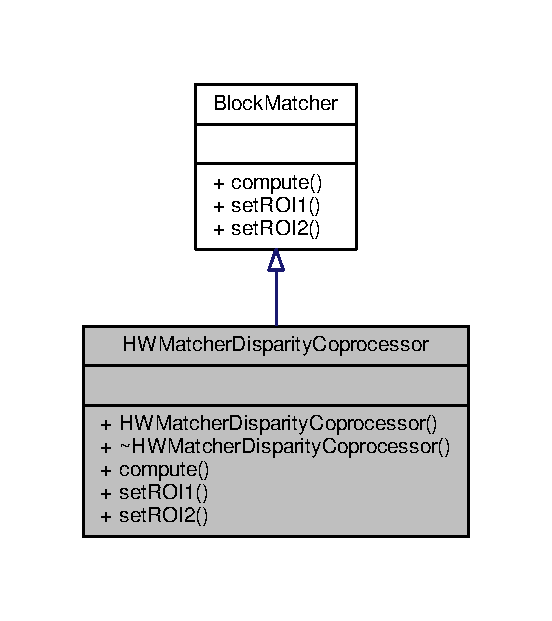
\includegraphics[width=265pt]{classHWMatcherDisparityCoprocessor__inherit__graph}
\end{center}
\end{figure}


Collaboration diagram for H\+W\+Matcher\+Disparity\+Coprocessor\+:
\nopagebreak
\begin{figure}[H]
\begin{center}
\leavevmode
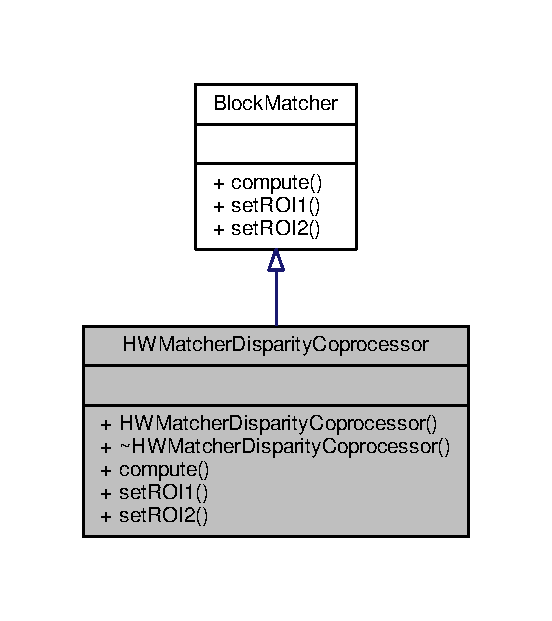
\includegraphics[width=265pt]{classHWMatcherDisparityCoprocessor__coll__graph}
\end{center}
\end{figure}
\subsection*{Public Member Functions}
\begin{DoxyCompactItemize}
\item 
\hyperlink{classHWMatcherDisparityCoprocessor_aed90204f067508f43844fef2d8fb53d3}{H\+W\+Matcher\+Disparity\+Coprocessor} (const char $\ast$uio\+\_\+name, int width, int height)
\item 
\hyperlink{classHWMatcherDisparityCoprocessor_a4cea3866b2afcc2ad604626f9d4ee5f7}{$\sim$\+H\+W\+Matcher\+Disparity\+Coprocessor} ()
\item 
int \hyperlink{classHWMatcherDisparityCoprocessor_a99cea617f78dbc9807e926b818103cc9}{compute} (Input\+Array left, Input\+Array right, Output\+Array out)
\item 
void \hyperlink{classHWMatcherDisparityCoprocessor_a3e267ddaad5c676e065c751d983efbf3}{set\+R\+O\+I1} (cv\+::\+Rect roi1)
\item 
void \hyperlink{classHWMatcherDisparityCoprocessor_af0eed2c0ada37722bbf7376369ace242}{set\+R\+O\+I2} (cv\+::\+Rect roi2)
\end{DoxyCompactItemize}


\subsection{Constructor \& Destructor Documentation}
\index{H\+W\+Matcher\+Disparity\+Coprocessor@{H\+W\+Matcher\+Disparity\+Coprocessor}!H\+W\+Matcher\+Disparity\+Coprocessor@{H\+W\+Matcher\+Disparity\+Coprocessor}}
\index{H\+W\+Matcher\+Disparity\+Coprocessor@{H\+W\+Matcher\+Disparity\+Coprocessor}!H\+W\+Matcher\+Disparity\+Coprocessor@{H\+W\+Matcher\+Disparity\+Coprocessor}}
\subsubsection[{\texorpdfstring{H\+W\+Matcher\+Disparity\+Coprocessor(const char $\ast$uio\+\_\+name, int width, int height)}{HWMatcherDisparityCoprocessor(const char *uio_name, int width, int height)}}]{\setlength{\rightskip}{0pt plus 5cm}H\+W\+Matcher\+Disparity\+Coprocessor\+::\+H\+W\+Matcher\+Disparity\+Coprocessor (
\begin{DoxyParamCaption}
\item[{const char $\ast$}]{uio\+\_\+name, }
\item[{int}]{width, }
\item[{int}]{height}
\end{DoxyParamCaption}
)}\hypertarget{classHWMatcherDisparityCoprocessor_aed90204f067508f43844fef2d8fb53d3}{}\label{classHWMatcherDisparityCoprocessor_aed90204f067508f43844fef2d8fb53d3}
\index{H\+W\+Matcher\+Disparity\+Coprocessor@{H\+W\+Matcher\+Disparity\+Coprocessor}!````~H\+W\+Matcher\+Disparity\+Coprocessor@{$\sim$\+H\+W\+Matcher\+Disparity\+Coprocessor}}
\index{````~H\+W\+Matcher\+Disparity\+Coprocessor@{$\sim$\+H\+W\+Matcher\+Disparity\+Coprocessor}!H\+W\+Matcher\+Disparity\+Coprocessor@{H\+W\+Matcher\+Disparity\+Coprocessor}}
\subsubsection[{\texorpdfstring{$\sim$\+H\+W\+Matcher\+Disparity\+Coprocessor()}{~HWMatcherDisparityCoprocessor()}}]{\setlength{\rightskip}{0pt plus 5cm}H\+W\+Matcher\+Disparity\+Coprocessor\+::$\sim$\+H\+W\+Matcher\+Disparity\+Coprocessor (
\begin{DoxyParamCaption}
{}
\end{DoxyParamCaption}
)}\hypertarget{classHWMatcherDisparityCoprocessor_a4cea3866b2afcc2ad604626f9d4ee5f7}{}\label{classHWMatcherDisparityCoprocessor_a4cea3866b2afcc2ad604626f9d4ee5f7}


\subsection{Member Function Documentation}
\index{H\+W\+Matcher\+Disparity\+Coprocessor@{H\+W\+Matcher\+Disparity\+Coprocessor}!compute@{compute}}
\index{compute@{compute}!H\+W\+Matcher\+Disparity\+Coprocessor@{H\+W\+Matcher\+Disparity\+Coprocessor}}
\subsubsection[{\texorpdfstring{compute(\+Input\+Array left, Input\+Array right, Output\+Array out)}{compute(InputArray left, InputArray right, OutputArray out)}}]{\setlength{\rightskip}{0pt plus 5cm}int H\+W\+Matcher\+Disparity\+Coprocessor\+::compute (
\begin{DoxyParamCaption}
\item[{Input\+Array}]{left, }
\item[{Input\+Array}]{right, }
\item[{Output\+Array}]{out}
\end{DoxyParamCaption}
)}\hypertarget{classHWMatcherDisparityCoprocessor_a99cea617f78dbc9807e926b818103cc9}{}\label{classHWMatcherDisparityCoprocessor_a99cea617f78dbc9807e926b818103cc9}
\index{H\+W\+Matcher\+Disparity\+Coprocessor@{H\+W\+Matcher\+Disparity\+Coprocessor}!set\+R\+O\+I1@{set\+R\+O\+I1}}
\index{set\+R\+O\+I1@{set\+R\+O\+I1}!H\+W\+Matcher\+Disparity\+Coprocessor@{H\+W\+Matcher\+Disparity\+Coprocessor}}
\subsubsection[{\texorpdfstring{set\+R\+O\+I1(cv\+::\+Rect roi1)}{setROI1(cv::Rect roi1)}}]{\setlength{\rightskip}{0pt plus 5cm}void H\+W\+Matcher\+Disparity\+Coprocessor\+::set\+R\+O\+I1 (
\begin{DoxyParamCaption}
\item[{cv\+::\+Rect}]{roi1}
\end{DoxyParamCaption}
)\hspace{0.3cm}{\ttfamily [inline]}, {\ttfamily [virtual]}}\hypertarget{classHWMatcherDisparityCoprocessor_a3e267ddaad5c676e065c751d983efbf3}{}\label{classHWMatcherDisparityCoprocessor_a3e267ddaad5c676e065c751d983efbf3}


Implements \hyperlink{classBlockMatcher_a0b1c689296bea9085be223e53ba538a0}{Block\+Matcher}.

\index{H\+W\+Matcher\+Disparity\+Coprocessor@{H\+W\+Matcher\+Disparity\+Coprocessor}!set\+R\+O\+I2@{set\+R\+O\+I2}}
\index{set\+R\+O\+I2@{set\+R\+O\+I2}!H\+W\+Matcher\+Disparity\+Coprocessor@{H\+W\+Matcher\+Disparity\+Coprocessor}}
\subsubsection[{\texorpdfstring{set\+R\+O\+I2(cv\+::\+Rect roi2)}{setROI2(cv::Rect roi2)}}]{\setlength{\rightskip}{0pt plus 5cm}void H\+W\+Matcher\+Disparity\+Coprocessor\+::set\+R\+O\+I2 (
\begin{DoxyParamCaption}
\item[{cv\+::\+Rect}]{roi2}
\end{DoxyParamCaption}
)\hspace{0.3cm}{\ttfamily [inline]}, {\ttfamily [virtual]}}\hypertarget{classHWMatcherDisparityCoprocessor_af0eed2c0ada37722bbf7376369ace242}{}\label{classHWMatcherDisparityCoprocessor_af0eed2c0ada37722bbf7376369ace242}


Implements \hyperlink{classBlockMatcher_af80a89fda1b2fd2d78e75e7466dcbcca}{Block\+Matcher}.



The documentation for this class was generated from the following files\+:\begin{DoxyCompactItemize}
\item 
include/stereo-\/matcher/\hyperlink{bm-hw-ip_8h}{bm-\/hw-\/ip.\+h}\item 
stereo-\/matcher/\hyperlink{bm-hw-ip_8cpp}{bm-\/hw-\/ip.\+cpp}\end{DoxyCompactItemize}

\hypertarget{classHWMorphologicalFilterIPCore}{}\section{H\+W\+Morphological\+Filter\+I\+P\+Core Class Reference}
\label{classHWMorphologicalFilterIPCore}\index{H\+W\+Morphological\+Filter\+I\+P\+Core@{H\+W\+Morphological\+Filter\+I\+P\+Core}}


{\ttfamily \#include $<$mf-\/hw-\/ip.\+h$>$}



Inheritance diagram for H\+W\+Morphological\+Filter\+I\+P\+Core\+:
\nopagebreak
\begin{figure}[H]
\begin{center}
\leavevmode
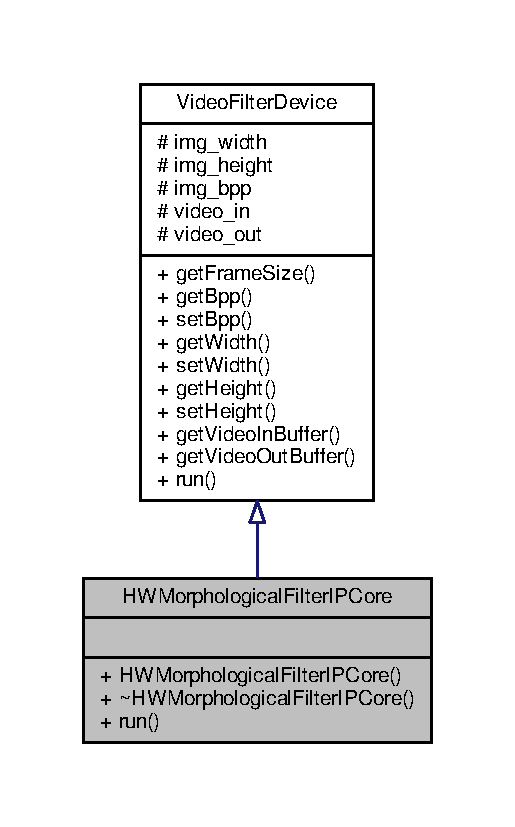
\includegraphics[width=247pt]{classHWMorphologicalFilterIPCore__inherit__graph}
\end{center}
\end{figure}


Collaboration diagram for H\+W\+Morphological\+Filter\+I\+P\+Core\+:
\nopagebreak
\begin{figure}[H]
\begin{center}
\leavevmode
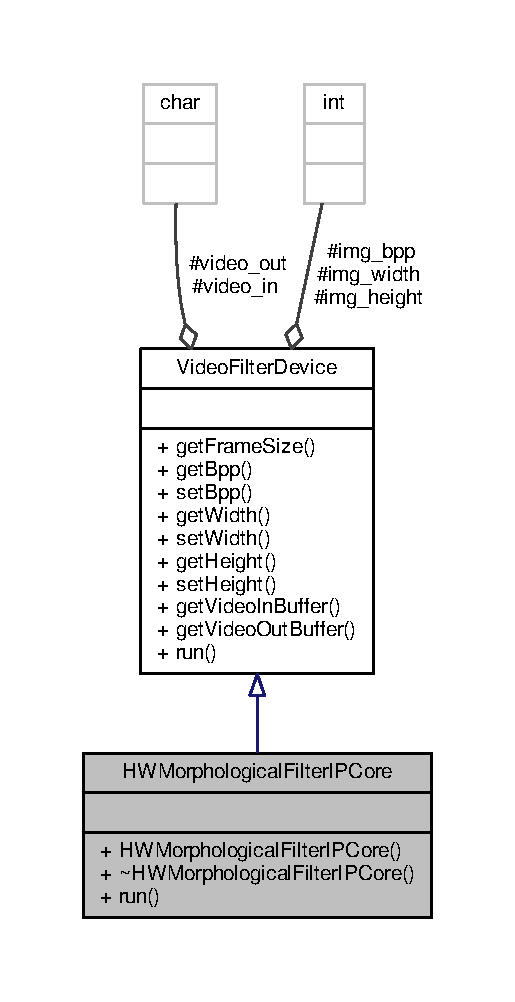
\includegraphics[width=247pt]{classHWMorphologicalFilterIPCore__coll__graph}
\end{center}
\end{figure}
\subsection*{Public Member Functions}
\begin{DoxyCompactItemize}
\item 
\hyperlink{classHWMorphologicalFilterIPCore_a337e6e3fee6b2a054885dd6b44afec9b}{H\+W\+Morphological\+Filter\+I\+P\+Core} (int w, int h, int bpp)
\item 
\hyperlink{classHWMorphologicalFilterIPCore_a9854c8ac2d7402ac9b20381c75678ae9}{$\sim$\+H\+W\+Morphological\+Filter\+I\+P\+Core} ()
\item 
int \hyperlink{classHWMorphologicalFilterIPCore_accac538b601dbc62a61b426b476cf4d0}{run} (cv\+::\+Input\+Array in, cv\+::\+Output\+Array out)
\end{DoxyCompactItemize}
\subsection*{Additional Inherited Members}


\subsection{Constructor \& Destructor Documentation}
\index{H\+W\+Morphological\+Filter\+I\+P\+Core@{H\+W\+Morphological\+Filter\+I\+P\+Core}!H\+W\+Morphological\+Filter\+I\+P\+Core@{H\+W\+Morphological\+Filter\+I\+P\+Core}}
\index{H\+W\+Morphological\+Filter\+I\+P\+Core@{H\+W\+Morphological\+Filter\+I\+P\+Core}!H\+W\+Morphological\+Filter\+I\+P\+Core@{H\+W\+Morphological\+Filter\+I\+P\+Core}}
\subsubsection[{\texorpdfstring{H\+W\+Morphological\+Filter\+I\+P\+Core(int w, int h, int bpp)}{HWMorphologicalFilterIPCore(int w, int h, int bpp)}}]{\setlength{\rightskip}{0pt plus 5cm}H\+W\+Morphological\+Filter\+I\+P\+Core\+::\+H\+W\+Morphological\+Filter\+I\+P\+Core (
\begin{DoxyParamCaption}
\item[{int}]{w, }
\item[{int}]{h, }
\item[{int}]{bpp}
\end{DoxyParamCaption}
)\hspace{0.3cm}{\ttfamily [explicit]}}\hypertarget{classHWMorphologicalFilterIPCore_a337e6e3fee6b2a054885dd6b44afec9b}{}\label{classHWMorphologicalFilterIPCore_a337e6e3fee6b2a054885dd6b44afec9b}
\index{H\+W\+Morphological\+Filter\+I\+P\+Core@{H\+W\+Morphological\+Filter\+I\+P\+Core}!````~H\+W\+Morphological\+Filter\+I\+P\+Core@{$\sim$\+H\+W\+Morphological\+Filter\+I\+P\+Core}}
\index{````~H\+W\+Morphological\+Filter\+I\+P\+Core@{$\sim$\+H\+W\+Morphological\+Filter\+I\+P\+Core}!H\+W\+Morphological\+Filter\+I\+P\+Core@{H\+W\+Morphological\+Filter\+I\+P\+Core}}
\subsubsection[{\texorpdfstring{$\sim$\+H\+W\+Morphological\+Filter\+I\+P\+Core()}{~HWMorphologicalFilterIPCore()}}]{\setlength{\rightskip}{0pt plus 5cm}H\+W\+Morphological\+Filter\+I\+P\+Core\+::$\sim$\+H\+W\+Morphological\+Filter\+I\+P\+Core (
\begin{DoxyParamCaption}
{}
\end{DoxyParamCaption}
)}\hypertarget{classHWMorphologicalFilterIPCore_a9854c8ac2d7402ac9b20381c75678ae9}{}\label{classHWMorphologicalFilterIPCore_a9854c8ac2d7402ac9b20381c75678ae9}


\subsection{Member Function Documentation}
\index{H\+W\+Morphological\+Filter\+I\+P\+Core@{H\+W\+Morphological\+Filter\+I\+P\+Core}!run@{run}}
\index{run@{run}!H\+W\+Morphological\+Filter\+I\+P\+Core@{H\+W\+Morphological\+Filter\+I\+P\+Core}}
\subsubsection[{\texorpdfstring{run(cv\+::\+Input\+Array in, cv\+::\+Output\+Array out)}{run(cv::InputArray in, cv::OutputArray out)}}]{\setlength{\rightskip}{0pt plus 5cm}int H\+W\+Morphological\+Filter\+I\+P\+Core\+::run (
\begin{DoxyParamCaption}
\item[{cv\+::\+Input\+Array}]{in, }
\item[{cv\+::\+Output\+Array}]{out}
\end{DoxyParamCaption}
)\hspace{0.3cm}{\ttfamily [virtual]}}\hypertarget{classHWMorphologicalFilterIPCore_accac538b601dbc62a61b426b476cf4d0}{}\label{classHWMorphologicalFilterIPCore_accac538b601dbc62a61b426b476cf4d0}


Implements \hyperlink{classVideoFilterDevice_a8c0e8a16b0574b95ead26f9907073c8d}{Video\+Filter\+Device}.



The documentation for this class was generated from the following files\+:\begin{DoxyCompactItemize}
\item 
include/filter/\hyperlink{mf-hw-ip_8h}{mf-\/hw-\/ip.\+h}\item 
filter/\hyperlink{mf-hw-ip_8cpp}{mf-\/hw-\/ip.\+cpp}\end{DoxyCompactItemize}

\hypertarget{classMJPEGDecoderDevice}{}\section{M\+J\+P\+E\+G\+Decoder\+Device Class Reference}
\label{classMJPEGDecoderDevice}\index{M\+J\+P\+E\+G\+Decoder\+Device@{M\+J\+P\+E\+G\+Decoder\+Device}}


{\ttfamily \#include $<$mjpeg-\/decoder-\/sw.\+h$>$}



Inheritance diagram for M\+J\+P\+E\+G\+Decoder\+Device\+:
\nopagebreak
\begin{figure}[H]
\begin{center}
\leavevmode
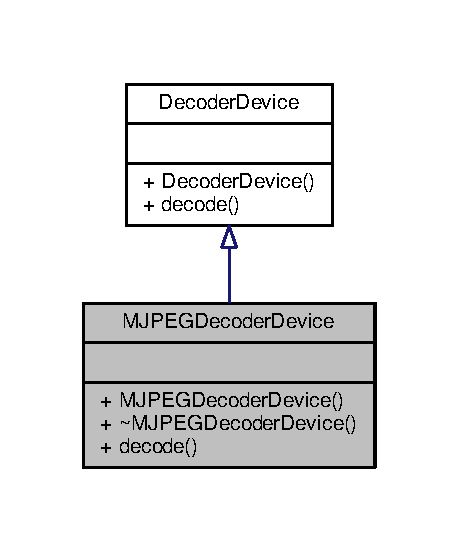
\includegraphics[width=220pt]{classMJPEGDecoderDevice__inherit__graph}
\end{center}
\end{figure}


Collaboration diagram for M\+J\+P\+E\+G\+Decoder\+Device\+:
\nopagebreak
\begin{figure}[H]
\begin{center}
\leavevmode
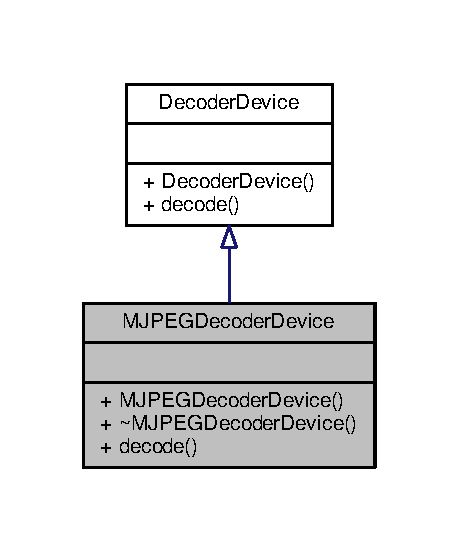
\includegraphics[width=220pt]{classMJPEGDecoderDevice__coll__graph}
\end{center}
\end{figure}
\subsection*{Public Member Functions}
\begin{DoxyCompactItemize}
\item 
\hyperlink{classMJPEGDecoderDevice_ad251c854ab5e757cff440b25fb5c8ddb}{M\+J\+P\+E\+G\+Decoder\+Device} ()
\item 
\hyperlink{classMJPEGDecoderDevice_aa86c079e207e6d5dd1013dc7b6437aae}{$\sim$\+M\+J\+P\+E\+G\+Decoder\+Device} ()
\item 
int \hyperlink{classMJPEGDecoderDevice_af765b926a83d573d5cf46a2c76d23597}{decode} (char $\ast$in, int len, int width, int height, char $\ast$out)
\end{DoxyCompactItemize}


\subsection{Constructor \& Destructor Documentation}
\index{M\+J\+P\+E\+G\+Decoder\+Device@{M\+J\+P\+E\+G\+Decoder\+Device}!M\+J\+P\+E\+G\+Decoder\+Device@{M\+J\+P\+E\+G\+Decoder\+Device}}
\index{M\+J\+P\+E\+G\+Decoder\+Device@{M\+J\+P\+E\+G\+Decoder\+Device}!M\+J\+P\+E\+G\+Decoder\+Device@{M\+J\+P\+E\+G\+Decoder\+Device}}
\subsubsection[{\texorpdfstring{M\+J\+P\+E\+G\+Decoder\+Device()}{MJPEGDecoderDevice()}}]{\setlength{\rightskip}{0pt plus 5cm}M\+J\+P\+E\+G\+Decoder\+Device\+::\+M\+J\+P\+E\+G\+Decoder\+Device (
\begin{DoxyParamCaption}
{}
\end{DoxyParamCaption}
)\hspace{0.3cm}{\ttfamily [explicit]}}\hypertarget{classMJPEGDecoderDevice_ad251c854ab5e757cff440b25fb5c8ddb}{}\label{classMJPEGDecoderDevice_ad251c854ab5e757cff440b25fb5c8ddb}
\index{M\+J\+P\+E\+G\+Decoder\+Device@{M\+J\+P\+E\+G\+Decoder\+Device}!````~M\+J\+P\+E\+G\+Decoder\+Device@{$\sim$\+M\+J\+P\+E\+G\+Decoder\+Device}}
\index{````~M\+J\+P\+E\+G\+Decoder\+Device@{$\sim$\+M\+J\+P\+E\+G\+Decoder\+Device}!M\+J\+P\+E\+G\+Decoder\+Device@{M\+J\+P\+E\+G\+Decoder\+Device}}
\subsubsection[{\texorpdfstring{$\sim$\+M\+J\+P\+E\+G\+Decoder\+Device()}{~MJPEGDecoderDevice()}}]{\setlength{\rightskip}{0pt plus 5cm}M\+J\+P\+E\+G\+Decoder\+Device\+::$\sim$\+M\+J\+P\+E\+G\+Decoder\+Device (
\begin{DoxyParamCaption}
{}
\end{DoxyParamCaption}
)}\hypertarget{classMJPEGDecoderDevice_aa86c079e207e6d5dd1013dc7b6437aae}{}\label{classMJPEGDecoderDevice_aa86c079e207e6d5dd1013dc7b6437aae}


\subsection{Member Function Documentation}
\index{M\+J\+P\+E\+G\+Decoder\+Device@{M\+J\+P\+E\+G\+Decoder\+Device}!decode@{decode}}
\index{decode@{decode}!M\+J\+P\+E\+G\+Decoder\+Device@{M\+J\+P\+E\+G\+Decoder\+Device}}
\subsubsection[{\texorpdfstring{decode(char $\ast$in, int len, int width, int height, char $\ast$out)}{decode(char *in, int len, int width, int height, char *out)}}]{\setlength{\rightskip}{0pt plus 5cm}int M\+J\+P\+E\+G\+Decoder\+Device\+::decode (
\begin{DoxyParamCaption}
\item[{char $\ast$}]{in, }
\item[{int}]{len, }
\item[{int}]{width, }
\item[{int}]{height, }
\item[{char $\ast$}]{out}
\end{DoxyParamCaption}
)\hspace{0.3cm}{\ttfamily [virtual]}}\hypertarget{classMJPEGDecoderDevice_af765b926a83d573d5cf46a2c76d23597}{}\label{classMJPEGDecoderDevice_af765b926a83d573d5cf46a2c76d23597}


Implements \hyperlink{classDecoderDevice_aadb33964bae3c6d9ad310105242d5611}{Decoder\+Device}.



The documentation for this class was generated from the following files\+:\begin{DoxyCompactItemize}
\item 
include/decoder/\hyperlink{mjpeg-decoder-sw_8h}{mjpeg-\/decoder-\/sw.\+h}\item 
decoder/\hyperlink{mjpeg-decoder-sw_8cpp}{mjpeg-\/decoder-\/sw.\+cpp}\end{DoxyCompactItemize}

\hypertarget{classSWMatcherKonolige}{}\section{S\+W\+Matcher\+Konolige Class Reference}
\label{classSWMatcherKonolige}\index{S\+W\+Matcher\+Konolige@{S\+W\+Matcher\+Konolige}}


{\ttfamily \#include $<$bm-\/sw.\+h$>$}



Inheritance diagram for S\+W\+Matcher\+Konolige\+:
\nopagebreak
\begin{figure}[H]
\begin{center}
\leavevmode
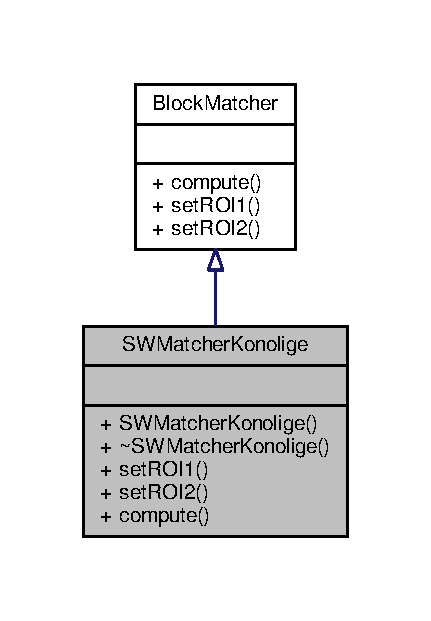
\includegraphics[width=207pt]{classSWMatcherKonolige__inherit__graph}
\end{center}
\end{figure}


Collaboration diagram for S\+W\+Matcher\+Konolige\+:
\nopagebreak
\begin{figure}[H]
\begin{center}
\leavevmode
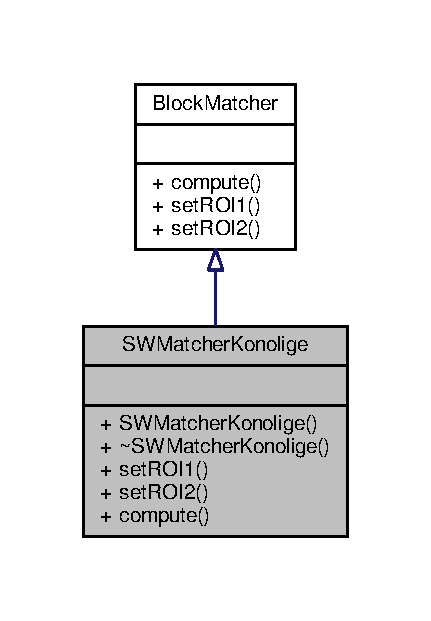
\includegraphics[width=207pt]{classSWMatcherKonolige__coll__graph}
\end{center}
\end{figure}
\subsection*{Public Member Functions}
\begin{DoxyCompactItemize}
\item 
\hyperlink{classSWMatcherKonolige_a3938a2b9d77d4d574bc4296daca7b409}{S\+W\+Matcher\+Konolige} (Rect \&roi1, Rect \&roi2, int pre\+Filter\+Cap, int block\+Size, int min\+Disparity, int texture\+Threshold, int num\+Of\+Disparities, int max\+Disparity, int uniqueness\+Ratio, int speckle\+Window\+Size, int speckle\+Range, int disp12\+Max\+Diff)
\item 
\hyperlink{classSWMatcherKonolige_a038a394f2854a3603c688db0b3f04d7b}{$\sim$\+S\+W\+Matcher\+Konolige} ()
\item 
void \hyperlink{classSWMatcherKonolige_a70a376f1d07da7000ea0a88fc3ab673a}{set\+R\+O\+I1} (cv\+::\+Rect roi1)
\item 
void \hyperlink{classSWMatcherKonolige_a05913005c4d1b5ea6b1bbcb79deef7d0}{set\+R\+O\+I2} (cv\+::\+Rect roi2)
\item 
int \hyperlink{classSWMatcherKonolige_a5df1e9c785130466ae316bae7763864b}{compute} (Input\+Array left, Input\+Array right, Output\+Array out)
\end{DoxyCompactItemize}


\subsection{Constructor \& Destructor Documentation}
\index{S\+W\+Matcher\+Konolige@{S\+W\+Matcher\+Konolige}!S\+W\+Matcher\+Konolige@{S\+W\+Matcher\+Konolige}}
\index{S\+W\+Matcher\+Konolige@{S\+W\+Matcher\+Konolige}!S\+W\+Matcher\+Konolige@{S\+W\+Matcher\+Konolige}}
\subsubsection[{\texorpdfstring{S\+W\+Matcher\+Konolige(\+Rect \&roi1, Rect \&roi2, int pre\+Filter\+Cap, int block\+Size, int min\+Disparity, int texture\+Threshold, int num\+Of\+Disparities, int max\+Disparity, int uniqueness\+Ratio, int speckle\+Window\+Size, int speckle\+Range, int disp12\+Max\+Diff)}{SWMatcherKonolige(Rect &roi1, Rect &roi2, int preFilterCap, int blockSize, int minDisparity, int textureThreshold, int numOfDisparities, int maxDisparity, int uniquenessRatio, int speckleWindowSize, int speckleRange, int disp12MaxDiff)}}]{\setlength{\rightskip}{0pt plus 5cm}S\+W\+Matcher\+Konolige\+::\+S\+W\+Matcher\+Konolige (
\begin{DoxyParamCaption}
\item[{Rect \&}]{roi1, }
\item[{Rect \&}]{roi2, }
\item[{int}]{pre\+Filter\+Cap, }
\item[{int}]{block\+Size, }
\item[{int}]{min\+Disparity, }
\item[{int}]{texture\+Threshold, }
\item[{int}]{num\+Of\+Disparities, }
\item[{int}]{max\+Disparity, }
\item[{int}]{uniqueness\+Ratio, }
\item[{int}]{speckle\+Window\+Size, }
\item[{int}]{speckle\+Range, }
\item[{int}]{disp12\+Max\+Diff}
\end{DoxyParamCaption}
)}\hypertarget{classSWMatcherKonolige_a3938a2b9d77d4d574bc4296daca7b409}{}\label{classSWMatcherKonolige_a3938a2b9d77d4d574bc4296daca7b409}
\index{S\+W\+Matcher\+Konolige@{S\+W\+Matcher\+Konolige}!````~S\+W\+Matcher\+Konolige@{$\sim$\+S\+W\+Matcher\+Konolige}}
\index{````~S\+W\+Matcher\+Konolige@{$\sim$\+S\+W\+Matcher\+Konolige}!S\+W\+Matcher\+Konolige@{S\+W\+Matcher\+Konolige}}
\subsubsection[{\texorpdfstring{$\sim$\+S\+W\+Matcher\+Konolige()}{~SWMatcherKonolige()}}]{\setlength{\rightskip}{0pt plus 5cm}S\+W\+Matcher\+Konolige\+::$\sim$\+S\+W\+Matcher\+Konolige (
\begin{DoxyParamCaption}
{}
\end{DoxyParamCaption}
)}\hypertarget{classSWMatcherKonolige_a038a394f2854a3603c688db0b3f04d7b}{}\label{classSWMatcherKonolige_a038a394f2854a3603c688db0b3f04d7b}


\subsection{Member Function Documentation}
\index{S\+W\+Matcher\+Konolige@{S\+W\+Matcher\+Konolige}!compute@{compute}}
\index{compute@{compute}!S\+W\+Matcher\+Konolige@{S\+W\+Matcher\+Konolige}}
\subsubsection[{\texorpdfstring{compute(\+Input\+Array left, Input\+Array right, Output\+Array out)}{compute(InputArray left, InputArray right, OutputArray out)}}]{\setlength{\rightskip}{0pt plus 5cm}int S\+W\+Matcher\+Konolige\+::compute (
\begin{DoxyParamCaption}
\item[{Input\+Array}]{left, }
\item[{Input\+Array}]{right, }
\item[{Output\+Array}]{out}
\end{DoxyParamCaption}
)}\hypertarget{classSWMatcherKonolige_a5df1e9c785130466ae316bae7763864b}{}\label{classSWMatcherKonolige_a5df1e9c785130466ae316bae7763864b}
\index{S\+W\+Matcher\+Konolige@{S\+W\+Matcher\+Konolige}!set\+R\+O\+I1@{set\+R\+O\+I1}}
\index{set\+R\+O\+I1@{set\+R\+O\+I1}!S\+W\+Matcher\+Konolige@{S\+W\+Matcher\+Konolige}}
\subsubsection[{\texorpdfstring{set\+R\+O\+I1(cv\+::\+Rect roi1)}{setROI1(cv::Rect roi1)}}]{\setlength{\rightskip}{0pt plus 5cm}void S\+W\+Matcher\+Konolige\+::set\+R\+O\+I1 (
\begin{DoxyParamCaption}
\item[{cv\+::\+Rect}]{roi1}
\end{DoxyParamCaption}
)\hspace{0.3cm}{\ttfamily [virtual]}}\hypertarget{classSWMatcherKonolige_a70a376f1d07da7000ea0a88fc3ab673a}{}\label{classSWMatcherKonolige_a70a376f1d07da7000ea0a88fc3ab673a}


Implements \hyperlink{classBlockMatcher_a0b1c689296bea9085be223e53ba538a0}{Block\+Matcher}.

\index{S\+W\+Matcher\+Konolige@{S\+W\+Matcher\+Konolige}!set\+R\+O\+I2@{set\+R\+O\+I2}}
\index{set\+R\+O\+I2@{set\+R\+O\+I2}!S\+W\+Matcher\+Konolige@{S\+W\+Matcher\+Konolige}}
\subsubsection[{\texorpdfstring{set\+R\+O\+I2(cv\+::\+Rect roi2)}{setROI2(cv::Rect roi2)}}]{\setlength{\rightskip}{0pt plus 5cm}void S\+W\+Matcher\+Konolige\+::set\+R\+O\+I2 (
\begin{DoxyParamCaption}
\item[{cv\+::\+Rect}]{roi2}
\end{DoxyParamCaption}
)\hspace{0.3cm}{\ttfamily [virtual]}}\hypertarget{classSWMatcherKonolige_a05913005c4d1b5ea6b1bbcb79deef7d0}{}\label{classSWMatcherKonolige_a05913005c4d1b5ea6b1bbcb79deef7d0}


Implements \hyperlink{classBlockMatcher_af80a89fda1b2fd2d78e75e7466dcbcca}{Block\+Matcher}.



The documentation for this class was generated from the following files\+:\begin{DoxyCompactItemize}
\item 
include/stereo-\/matcher/\hyperlink{bm-sw_8h}{bm-\/sw.\+h}\item 
stereo-\/matcher/\hyperlink{bm-sw_8cpp}{bm-\/sw.\+cpp}\end{DoxyCompactItemize}

\hypertarget{classSWMorphologicalFilter}{}\section{S\+W\+Morphological\+Filter Class Reference}
\label{classSWMorphologicalFilter}\index{S\+W\+Morphological\+Filter@{S\+W\+Morphological\+Filter}}


{\ttfamily \#include $<$mf-\/sw.\+h$>$}



Inheritance diagram for S\+W\+Morphological\+Filter\+:
\nopagebreak
\begin{figure}[H]
\begin{center}
\leavevmode
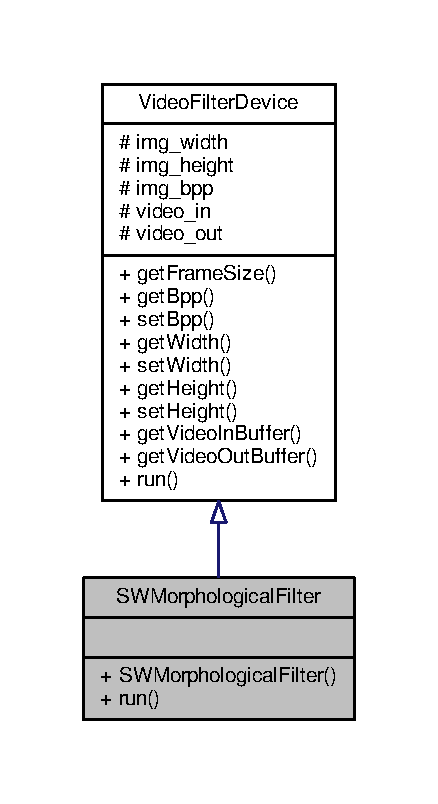
\includegraphics[width=210pt]{classSWMorphologicalFilter__inherit__graph}
\end{center}
\end{figure}


Collaboration diagram for S\+W\+Morphological\+Filter\+:
\nopagebreak
\begin{figure}[H]
\begin{center}
\leavevmode
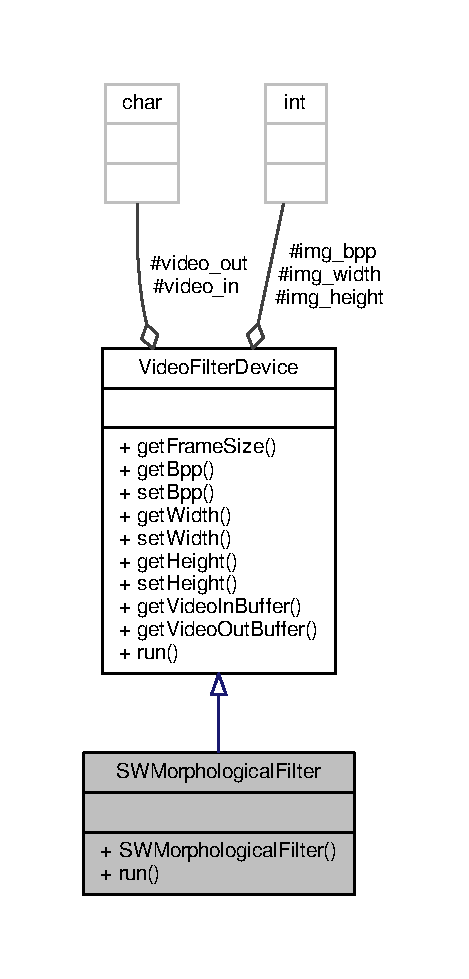
\includegraphics[width=225pt]{classSWMorphologicalFilter__coll__graph}
\end{center}
\end{figure}
\subsection*{Public Member Functions}
\begin{DoxyCompactItemize}
\item 
\hyperlink{classSWMorphologicalFilter_a0ac1de93747948924af5ff8bf5b539de}{S\+W\+Morphological\+Filter} (int w, int h, int bpp)
\item 
int \hyperlink{classSWMorphologicalFilter_a6c7ebdba2bbcd4e80aff2c3f2337f972}{run} (cv\+::\+Input\+Array in, cv\+::\+Output\+Array out)
\end{DoxyCompactItemize}
\subsection*{Additional Inherited Members}


\subsection{Constructor \& Destructor Documentation}
\index{S\+W\+Morphological\+Filter@{S\+W\+Morphological\+Filter}!S\+W\+Morphological\+Filter@{S\+W\+Morphological\+Filter}}
\index{S\+W\+Morphological\+Filter@{S\+W\+Morphological\+Filter}!S\+W\+Morphological\+Filter@{S\+W\+Morphological\+Filter}}
\subsubsection[{\texorpdfstring{S\+W\+Morphological\+Filter(int w, int h, int bpp)}{SWMorphologicalFilter(int w, int h, int bpp)}}]{\setlength{\rightskip}{0pt plus 5cm}S\+W\+Morphological\+Filter\+::\+S\+W\+Morphological\+Filter (
\begin{DoxyParamCaption}
\item[{int}]{w, }
\item[{int}]{h, }
\item[{int}]{bpp}
\end{DoxyParamCaption}
)\hspace{0.3cm}{\ttfamily [explicit]}}\hypertarget{classSWMorphologicalFilter_a0ac1de93747948924af5ff8bf5b539de}{}\label{classSWMorphologicalFilter_a0ac1de93747948924af5ff8bf5b539de}


\subsection{Member Function Documentation}
\index{S\+W\+Morphological\+Filter@{S\+W\+Morphological\+Filter}!run@{run}}
\index{run@{run}!S\+W\+Morphological\+Filter@{S\+W\+Morphological\+Filter}}
\subsubsection[{\texorpdfstring{run(cv\+::\+Input\+Array in, cv\+::\+Output\+Array out)}{run(cv::InputArray in, cv::OutputArray out)}}]{\setlength{\rightskip}{0pt plus 5cm}int S\+W\+Morphological\+Filter\+::run (
\begin{DoxyParamCaption}
\item[{cv\+::\+Input\+Array}]{in, }
\item[{cv\+::\+Output\+Array}]{out}
\end{DoxyParamCaption}
)\hspace{0.3cm}{\ttfamily [virtual]}}\hypertarget{classSWMorphologicalFilter_a6c7ebdba2bbcd4e80aff2c3f2337f972}{}\label{classSWMorphologicalFilter_a6c7ebdba2bbcd4e80aff2c3f2337f972}


Implements \hyperlink{classVideoFilterDevice_a8c0e8a16b0574b95ead26f9907073c8d}{Video\+Filter\+Device}.



The documentation for this class was generated from the following files\+:\begin{DoxyCompactItemize}
\item 
include/filter/\hyperlink{mf-sw_8h}{mf-\/sw.\+h}\item 
filter/\hyperlink{mf-sw_8cpp}{mf-\/sw.\+cpp}\end{DoxyCompactItemize}

\hypertarget{classSWSemiGlobalMatcher}{}\section{S\+W\+Semi\+Global\+Matcher Class Reference}
\label{classSWSemiGlobalMatcher}\index{S\+W\+Semi\+Global\+Matcher@{S\+W\+Semi\+Global\+Matcher}}


{\ttfamily \#include $<$sgbm-\/sw.\+h$>$}



Inheritance diagram for S\+W\+Semi\+Global\+Matcher\+:
\nopagebreak
\begin{figure}[H]
\begin{center}
\leavevmode
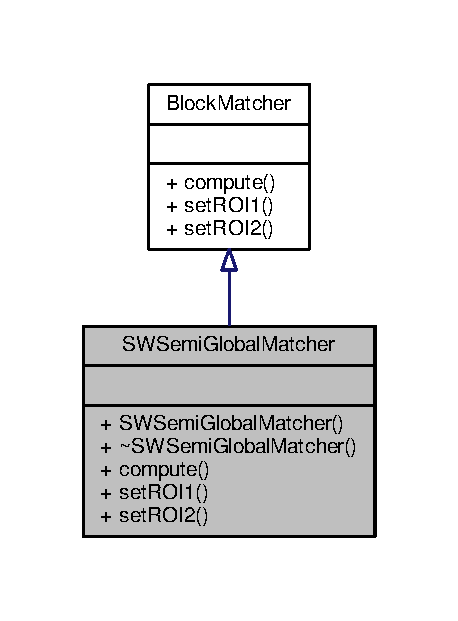
\includegraphics[width=220pt]{classSWSemiGlobalMatcher__inherit__graph}
\end{center}
\end{figure}


Collaboration diagram for S\+W\+Semi\+Global\+Matcher\+:
\nopagebreak
\begin{figure}[H]
\begin{center}
\leavevmode
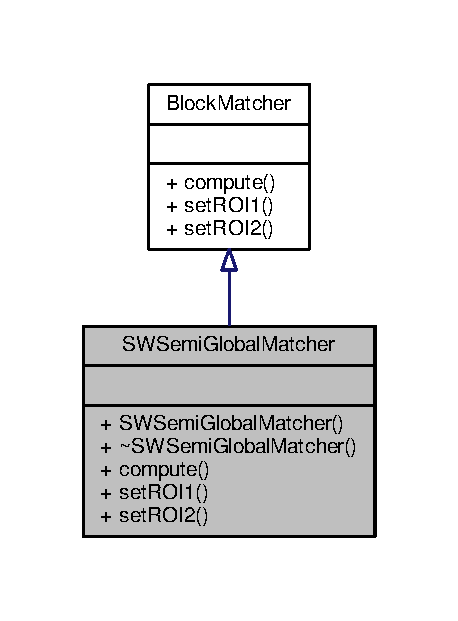
\includegraphics[width=220pt]{classSWSemiGlobalMatcher__coll__graph}
\end{center}
\end{figure}
\subsection*{Public Member Functions}
\begin{DoxyCompactItemize}
\item 
\hyperlink{classSWSemiGlobalMatcher_a8ceda1c4cffa5b5df7540f0e8efccc7c}{S\+W\+Semi\+Global\+Matcher} (int block\+Size, int min\+Disparity, int num\+Of\+Disparities, int uniqueness\+Ratio, int speckle\+Window\+Size, int speckle\+Range, int disp12\+Max\+Diff)
\item 
\hyperlink{classSWSemiGlobalMatcher_a77760cac2e94267ca6c8de7511eed163}{$\sim$\+S\+W\+Semi\+Global\+Matcher} ()
\item 
int \hyperlink{classSWSemiGlobalMatcher_a08419285671190aad745993fa6d8724e}{compute} (Input\+Array left, Input\+Array right, Output\+Array out)
\item 
void \hyperlink{classSWSemiGlobalMatcher_a67bf29294ea497441037616b1fb32769}{set\+R\+O\+I1} (cv\+::\+Rect roi1)
\item 
void \hyperlink{classSWSemiGlobalMatcher_a8cfa467d703b6a38cbd9e3ff1f9a3f70}{set\+R\+O\+I2} (cv\+::\+Rect roi2)
\end{DoxyCompactItemize}


\subsection{Constructor \& Destructor Documentation}
\index{S\+W\+Semi\+Global\+Matcher@{S\+W\+Semi\+Global\+Matcher}!S\+W\+Semi\+Global\+Matcher@{S\+W\+Semi\+Global\+Matcher}}
\index{S\+W\+Semi\+Global\+Matcher@{S\+W\+Semi\+Global\+Matcher}!S\+W\+Semi\+Global\+Matcher@{S\+W\+Semi\+Global\+Matcher}}
\subsubsection[{\texorpdfstring{S\+W\+Semi\+Global\+Matcher(int block\+Size, int min\+Disparity, int num\+Of\+Disparities, int uniqueness\+Ratio, int speckle\+Window\+Size, int speckle\+Range, int disp12\+Max\+Diff)}{SWSemiGlobalMatcher(int blockSize, int minDisparity, int numOfDisparities, int uniquenessRatio, int speckleWindowSize, int speckleRange, int disp12MaxDiff)}}]{\setlength{\rightskip}{0pt plus 5cm}S\+W\+Semi\+Global\+Matcher\+::\+S\+W\+Semi\+Global\+Matcher (
\begin{DoxyParamCaption}
\item[{int}]{block\+Size, }
\item[{int}]{min\+Disparity, }
\item[{int}]{num\+Of\+Disparities, }
\item[{int}]{uniqueness\+Ratio, }
\item[{int}]{speckle\+Window\+Size, }
\item[{int}]{speckle\+Range, }
\item[{int}]{disp12\+Max\+Diff}
\end{DoxyParamCaption}
)}\hypertarget{classSWSemiGlobalMatcher_a8ceda1c4cffa5b5df7540f0e8efccc7c}{}\label{classSWSemiGlobalMatcher_a8ceda1c4cffa5b5df7540f0e8efccc7c}
\index{S\+W\+Semi\+Global\+Matcher@{S\+W\+Semi\+Global\+Matcher}!````~S\+W\+Semi\+Global\+Matcher@{$\sim$\+S\+W\+Semi\+Global\+Matcher}}
\index{````~S\+W\+Semi\+Global\+Matcher@{$\sim$\+S\+W\+Semi\+Global\+Matcher}!S\+W\+Semi\+Global\+Matcher@{S\+W\+Semi\+Global\+Matcher}}
\subsubsection[{\texorpdfstring{$\sim$\+S\+W\+Semi\+Global\+Matcher()}{~SWSemiGlobalMatcher()}}]{\setlength{\rightskip}{0pt plus 5cm}S\+W\+Semi\+Global\+Matcher\+::$\sim$\+S\+W\+Semi\+Global\+Matcher (
\begin{DoxyParamCaption}
{}
\end{DoxyParamCaption}
)}\hypertarget{classSWSemiGlobalMatcher_a77760cac2e94267ca6c8de7511eed163}{}\label{classSWSemiGlobalMatcher_a77760cac2e94267ca6c8de7511eed163}


\subsection{Member Function Documentation}
\index{S\+W\+Semi\+Global\+Matcher@{S\+W\+Semi\+Global\+Matcher}!compute@{compute}}
\index{compute@{compute}!S\+W\+Semi\+Global\+Matcher@{S\+W\+Semi\+Global\+Matcher}}
\subsubsection[{\texorpdfstring{compute(\+Input\+Array left, Input\+Array right, Output\+Array out)}{compute(InputArray left, InputArray right, OutputArray out)}}]{\setlength{\rightskip}{0pt plus 5cm}int S\+W\+Semi\+Global\+Matcher\+::compute (
\begin{DoxyParamCaption}
\item[{Input\+Array}]{left, }
\item[{Input\+Array}]{right, }
\item[{Output\+Array}]{out}
\end{DoxyParamCaption}
)}\hypertarget{classSWSemiGlobalMatcher_a08419285671190aad745993fa6d8724e}{}\label{classSWSemiGlobalMatcher_a08419285671190aad745993fa6d8724e}
\index{S\+W\+Semi\+Global\+Matcher@{S\+W\+Semi\+Global\+Matcher}!set\+R\+O\+I1@{set\+R\+O\+I1}}
\index{set\+R\+O\+I1@{set\+R\+O\+I1}!S\+W\+Semi\+Global\+Matcher@{S\+W\+Semi\+Global\+Matcher}}
\subsubsection[{\texorpdfstring{set\+R\+O\+I1(cv\+::\+Rect roi1)}{setROI1(cv::Rect roi1)}}]{\setlength{\rightskip}{0pt plus 5cm}void S\+W\+Semi\+Global\+Matcher\+::set\+R\+O\+I1 (
\begin{DoxyParamCaption}
\item[{cv\+::\+Rect}]{roi1}
\end{DoxyParamCaption}
)\hspace{0.3cm}{\ttfamily [inline]}, {\ttfamily [virtual]}}\hypertarget{classSWSemiGlobalMatcher_a67bf29294ea497441037616b1fb32769}{}\label{classSWSemiGlobalMatcher_a67bf29294ea497441037616b1fb32769}


Implements \hyperlink{classBlockMatcher_a0b1c689296bea9085be223e53ba538a0}{Block\+Matcher}.

\index{S\+W\+Semi\+Global\+Matcher@{S\+W\+Semi\+Global\+Matcher}!set\+R\+O\+I2@{set\+R\+O\+I2}}
\index{set\+R\+O\+I2@{set\+R\+O\+I2}!S\+W\+Semi\+Global\+Matcher@{S\+W\+Semi\+Global\+Matcher}}
\subsubsection[{\texorpdfstring{set\+R\+O\+I2(cv\+::\+Rect roi2)}{setROI2(cv::Rect roi2)}}]{\setlength{\rightskip}{0pt plus 5cm}void S\+W\+Semi\+Global\+Matcher\+::set\+R\+O\+I2 (
\begin{DoxyParamCaption}
\item[{cv\+::\+Rect}]{roi2}
\end{DoxyParamCaption}
)\hspace{0.3cm}{\ttfamily [inline]}, {\ttfamily [virtual]}}\hypertarget{classSWSemiGlobalMatcher_a8cfa467d703b6a38cbd9e3ff1f9a3f70}{}\label{classSWSemiGlobalMatcher_a8cfa467d703b6a38cbd9e3ff1f9a3f70}


Implements \hyperlink{classBlockMatcher_af80a89fda1b2fd2d78e75e7466dcbcca}{Block\+Matcher}.



The documentation for this class was generated from the following files\+:\begin{DoxyCompactItemize}
\item 
include/stereo-\/matcher/\hyperlink{sgbm-sw_8h}{sgbm-\/sw.\+h}\item 
stereo-\/matcher/\hyperlink{sgbm-sw_8cpp}{sgbm-\/sw.\+cpp}\end{DoxyCompactItemize}

\hypertarget{classV4LStreamStereoDevice}{}\section{V4\+L\+Stream\+Stereo\+Device Class Reference}
\label{classV4LStreamStereoDevice}\index{V4\+L\+Stream\+Stereo\+Device@{V4\+L\+Stream\+Stereo\+Device}}


{\ttfamily \#include $<$v4l2-\/stream-\/stereo-\/device.\+h$>$}



Inheritance diagram for V4\+L\+Stream\+Stereo\+Device\+:
\nopagebreak
\begin{figure}[H]
\begin{center}
\leavevmode
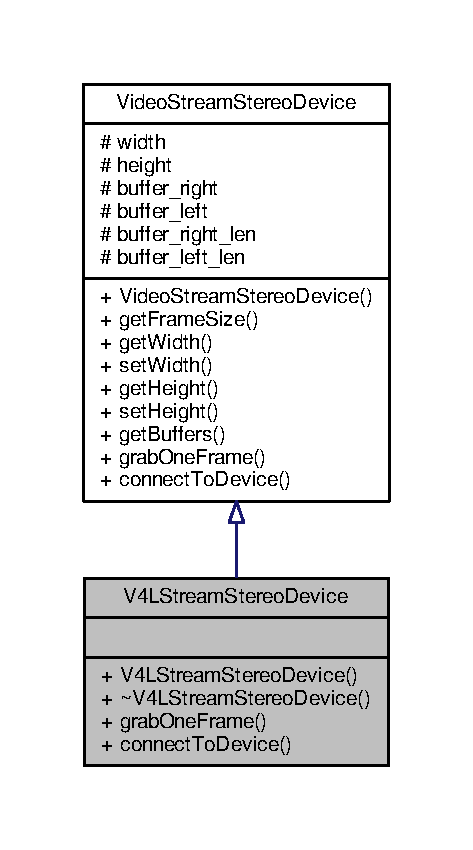
\includegraphics[width=227pt]{classV4LStreamStereoDevice__inherit__graph}
\end{center}
\end{figure}


Collaboration diagram for V4\+L\+Stream\+Stereo\+Device\+:
\nopagebreak
\begin{figure}[H]
\begin{center}
\leavevmode
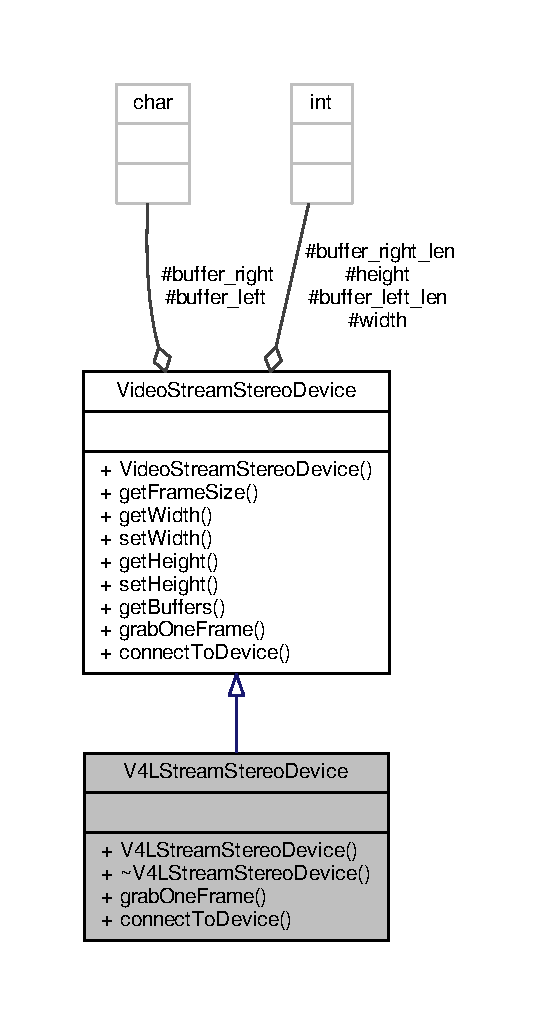
\includegraphics[width=260pt]{classV4LStreamStereoDevice__coll__graph}
\end{center}
\end{figure}
\subsection*{Public Member Functions}
\begin{DoxyCompactItemize}
\item 
\hyperlink{classV4LStreamStereoDevice_a8b5178fdbc4f381c088fdf2e7c098551}{V4\+L\+Stream\+Stereo\+Device} (std\+::string vdev\+\_\+right=\char`\"{}/dev/video0\char`\"{}, std\+::string vdev\+\_\+left=\char`\"{}/dev/video1\char`\"{}, int \hyperlink{classVideoStreamStereoDevice_a87596748c13021a3623bb55de4c9be14}{width}=640, int \hyperlink{classVideoStreamStereoDevice_a97af0c098374ce089e71d9020b792f1f}{height}=480)
\item 
\hyperlink{classV4LStreamStereoDevice_a27feadb2023f0293915353a749fa866d}{$\sim$\+V4\+L\+Stream\+Stereo\+Device} ()
\item 
int \hyperlink{classV4LStreamStereoDevice_af5170cee3401eb70e771b56fbf2104d7}{grab\+One\+Frame} ()
\item 
int \hyperlink{classV4LStreamStereoDevice_a0ecb2dd2636fcbfccc0e43604bf9bd14}{connect\+To\+Device} ()
\end{DoxyCompactItemize}
\subsection*{Additional Inherited Members}


\subsection{Constructor \& Destructor Documentation}
\index{V4\+L\+Stream\+Stereo\+Device@{V4\+L\+Stream\+Stereo\+Device}!V4\+L\+Stream\+Stereo\+Device@{V4\+L\+Stream\+Stereo\+Device}}
\index{V4\+L\+Stream\+Stereo\+Device@{V4\+L\+Stream\+Stereo\+Device}!V4\+L\+Stream\+Stereo\+Device@{V4\+L\+Stream\+Stereo\+Device}}
\subsubsection[{\texorpdfstring{V4\+L\+Stream\+Stereo\+Device(std\+::string vdev\+\_\+right=""/dev/video0"", std\+::string vdev\+\_\+left=""/dev/video1"", int width=640, int height=480)}{V4LStreamStereoDevice(std::string vdev_right="/dev/video0", std::string vdev_left="/dev/video1", int width=640, int height=480)}}]{\setlength{\rightskip}{0pt plus 5cm}V4\+L\+Stream\+Stereo\+Device\+::\+V4\+L\+Stream\+Stereo\+Device (
\begin{DoxyParamCaption}
\item[{std\+::string}]{vdev\+\_\+right = {\ttfamily \char`\"{}/dev/video0\char`\"{}}, }
\item[{std\+::string}]{vdev\+\_\+left = {\ttfamily \char`\"{}/dev/video1\char`\"{}}, }
\item[{int}]{width = {\ttfamily 640}, }
\item[{int}]{height = {\ttfamily 480}}
\end{DoxyParamCaption}
)}\hypertarget{classV4LStreamStereoDevice_a8b5178fdbc4f381c088fdf2e7c098551}{}\label{classV4LStreamStereoDevice_a8b5178fdbc4f381c088fdf2e7c098551}
\index{V4\+L\+Stream\+Stereo\+Device@{V4\+L\+Stream\+Stereo\+Device}!````~V4\+L\+Stream\+Stereo\+Device@{$\sim$\+V4\+L\+Stream\+Stereo\+Device}}
\index{````~V4\+L\+Stream\+Stereo\+Device@{$\sim$\+V4\+L\+Stream\+Stereo\+Device}!V4\+L\+Stream\+Stereo\+Device@{V4\+L\+Stream\+Stereo\+Device}}
\subsubsection[{\texorpdfstring{$\sim$\+V4\+L\+Stream\+Stereo\+Device()}{~V4LStreamStereoDevice()}}]{\setlength{\rightskip}{0pt plus 5cm}V4\+L\+Stream\+Stereo\+Device\+::$\sim$\+V4\+L\+Stream\+Stereo\+Device (
\begin{DoxyParamCaption}
{}
\end{DoxyParamCaption}
)}\hypertarget{classV4LStreamStereoDevice_a27feadb2023f0293915353a749fa866d}{}\label{classV4LStreamStereoDevice_a27feadb2023f0293915353a749fa866d}


\subsection{Member Function Documentation}
\index{V4\+L\+Stream\+Stereo\+Device@{V4\+L\+Stream\+Stereo\+Device}!connect\+To\+Device@{connect\+To\+Device}}
\index{connect\+To\+Device@{connect\+To\+Device}!V4\+L\+Stream\+Stereo\+Device@{V4\+L\+Stream\+Stereo\+Device}}
\subsubsection[{\texorpdfstring{connect\+To\+Device()}{connectToDevice()}}]{\setlength{\rightskip}{0pt plus 5cm}int V4\+L\+Stream\+Stereo\+Device\+::connect\+To\+Device (
\begin{DoxyParamCaption}
{}
\end{DoxyParamCaption}
)\hspace{0.3cm}{\ttfamily [virtual]}}\hypertarget{classV4LStreamStereoDevice_a0ecb2dd2636fcbfccc0e43604bf9bd14}{}\label{classV4LStreamStereoDevice_a0ecb2dd2636fcbfccc0e43604bf9bd14}


Implements \hyperlink{classVideoStreamStereoDevice_aa85f8836979a061a7f11d0e3ca0f9c44}{Video\+Stream\+Stereo\+Device}.

\index{V4\+L\+Stream\+Stereo\+Device@{V4\+L\+Stream\+Stereo\+Device}!grab\+One\+Frame@{grab\+One\+Frame}}
\index{grab\+One\+Frame@{grab\+One\+Frame}!V4\+L\+Stream\+Stereo\+Device@{V4\+L\+Stream\+Stereo\+Device}}
\subsubsection[{\texorpdfstring{grab\+One\+Frame()}{grabOneFrame()}}]{\setlength{\rightskip}{0pt plus 5cm}int V4\+L\+Stream\+Stereo\+Device\+::grab\+One\+Frame (
\begin{DoxyParamCaption}
{}
\end{DoxyParamCaption}
)\hspace{0.3cm}{\ttfamily [virtual]}}\hypertarget{classV4LStreamStereoDevice_af5170cee3401eb70e771b56fbf2104d7}{}\label{classV4LStreamStereoDevice_af5170cee3401eb70e771b56fbf2104d7}


Implements \hyperlink{classVideoStreamStereoDevice_a98ac1bfc13c0d700ee8f4658485e0d39}{Video\+Stream\+Stereo\+Device}.



The documentation for this class was generated from the following files\+:\begin{DoxyCompactItemize}
\item 
include/stream/\hyperlink{v4l2-stream-stereo-device_8h}{v4l2-\/stream-\/stereo-\/device.\+h}\item 
stream/\hyperlink{v4l2-stream-stereo-device_8cpp}{v4l2-\/stream-\/stereo-\/device.\+cpp}\end{DoxyCompactItemize}

\hypertarget{structvdma__transfer__dim}{}\section{vdma\+\_\+transfer\+\_\+dim Struct Reference}
\label{structvdma__transfer__dim}\index{vdma\+\_\+transfer\+\_\+dim@{vdma\+\_\+transfer\+\_\+dim}}


{\ttfamily \#include $<$mf-\/hw-\/ip.\+h$>$}



Collaboration diagram for vdma\+\_\+transfer\+\_\+dim\+:
\nopagebreak
\begin{figure}[H]
\begin{center}
\leavevmode
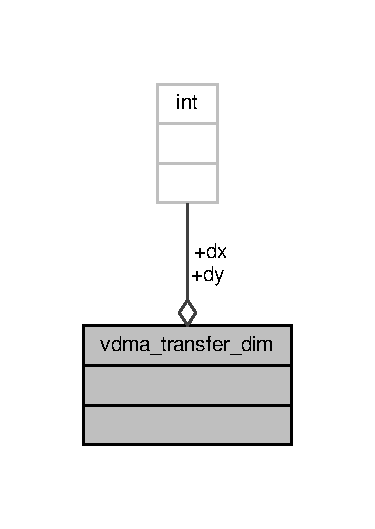
\includegraphics[width=180pt]{structvdma__transfer__dim__coll__graph}
\end{center}
\end{figure}
\subsection*{Public Attributes}
\begin{DoxyCompactItemize}
\item 
int \hyperlink{structvdma__transfer__dim_a35aa29bbfcd3f86ed0bd78c9bf32cb71}{dx}
\item 
int \hyperlink{structvdma__transfer__dim_aa036b394a5a9b51a283bc55e9211a7e8}{dy}
\end{DoxyCompactItemize}


\subsection{Member Data Documentation}
\index{vdma\+\_\+transfer\+\_\+dim@{vdma\+\_\+transfer\+\_\+dim}!dx@{dx}}
\index{dx@{dx}!vdma\+\_\+transfer\+\_\+dim@{vdma\+\_\+transfer\+\_\+dim}}
\subsubsection[{\texorpdfstring{dx}{dx}}]{\setlength{\rightskip}{0pt plus 5cm}int vdma\+\_\+transfer\+\_\+dim\+::dx}\hypertarget{structvdma__transfer__dim_a35aa29bbfcd3f86ed0bd78c9bf32cb71}{}\label{structvdma__transfer__dim_a35aa29bbfcd3f86ed0bd78c9bf32cb71}
\index{vdma\+\_\+transfer\+\_\+dim@{vdma\+\_\+transfer\+\_\+dim}!dy@{dy}}
\index{dy@{dy}!vdma\+\_\+transfer\+\_\+dim@{vdma\+\_\+transfer\+\_\+dim}}
\subsubsection[{\texorpdfstring{dy}{dy}}]{\setlength{\rightskip}{0pt plus 5cm}int vdma\+\_\+transfer\+\_\+dim\+::dy}\hypertarget{structvdma__transfer__dim_aa036b394a5a9b51a283bc55e9211a7e8}{}\label{structvdma__transfer__dim_aa036b394a5a9b51a283bc55e9211a7e8}


The documentation for this struct was generated from the following file\+:\begin{DoxyCompactItemize}
\item 
include/filter/\hyperlink{mf-hw-ip_8h}{mf-\/hw-\/ip.\+h}\end{DoxyCompactItemize}

\hypertarget{classVideoFilterDevice}{}\section{Video\+Filter\+Device Class Reference}
\label{classVideoFilterDevice}\index{Video\+Filter\+Device@{Video\+Filter\+Device}}


{\ttfamily \#include $<$filter.\+h$>$}



Inheritance diagram for Video\+Filter\+Device\+:
\nopagebreak
\begin{figure}[H]
\begin{center}
\leavevmode
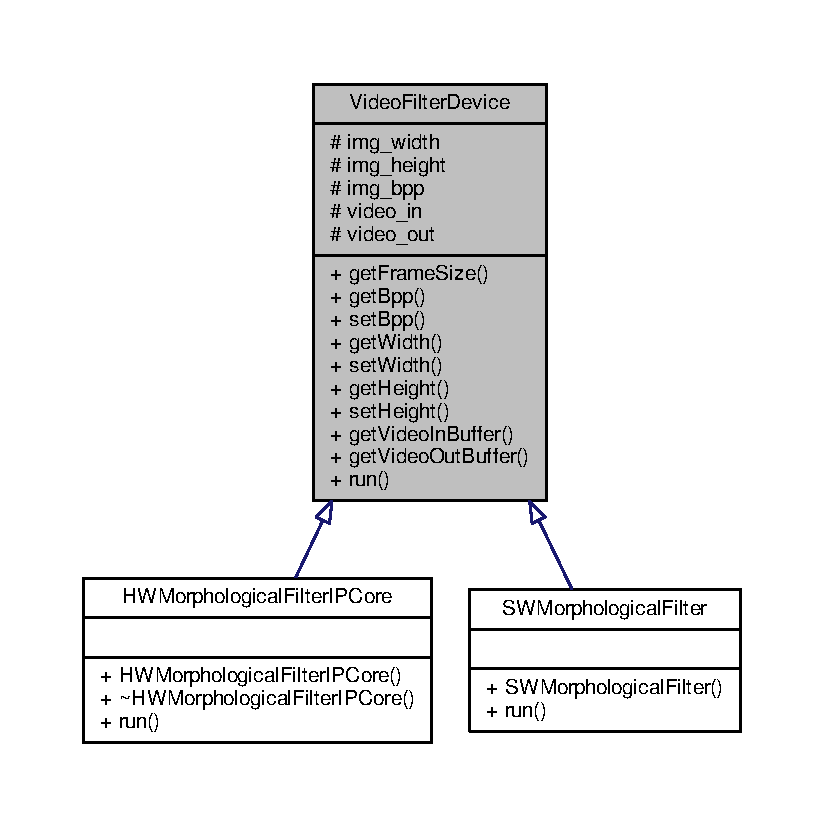
\includegraphics[width=350pt]{classVideoFilterDevice__inherit__graph}
\end{center}
\end{figure}


Collaboration diagram for Video\+Filter\+Device\+:
\nopagebreak
\begin{figure}[H]
\begin{center}
\leavevmode
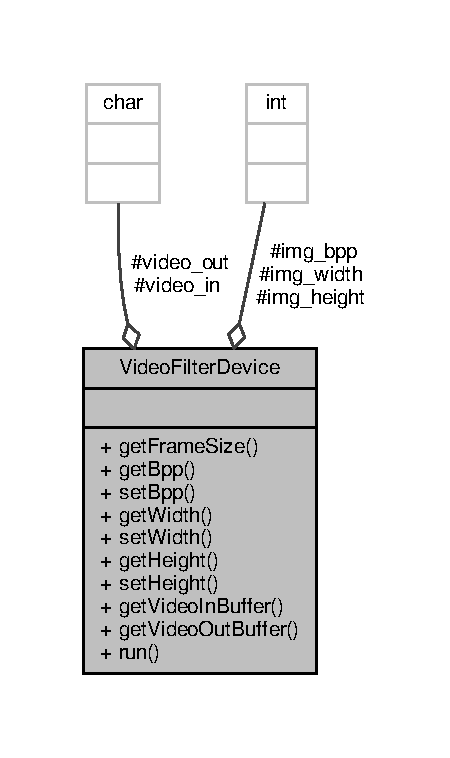
\includegraphics[width=216pt]{classVideoFilterDevice__coll__graph}
\end{center}
\end{figure}
\subsection*{Public Member Functions}
\begin{DoxyCompactItemize}
\item 
int \hyperlink{classVideoFilterDevice_a58e42daac01703e19465afd151a5e363}{get\+Frame\+Size} () const 
\item 
int \hyperlink{classVideoFilterDevice_a49cae600ea3be005491f0578e7c63863}{get\+Bpp} () const 
\item 
void \hyperlink{classVideoFilterDevice_a61c87ce1026569c72eab67ec1cd1140d}{set\+Bpp} (int bpp)
\item 
int \hyperlink{classVideoFilterDevice_a8dd4132ce498d59b867d661fc86d250e}{get\+Width} () const 
\item 
void \hyperlink{classVideoFilterDevice_a15f788f1d03a0fa1b44c594f4e0a3c48}{set\+Width} (int value)
\item 
int \hyperlink{classVideoFilterDevice_ac8ca39177708cc8d1069aa20744fbbeb}{get\+Height} () const 
\item 
void \hyperlink{classVideoFilterDevice_a1c054f9e2254c17b017e81c858a5e6be}{set\+Height} (int value)
\item 
char $\ast$ \hyperlink{classVideoFilterDevice_ac6828e9cb7f42934adbb6b278a3219c0}{get\+Video\+In\+Buffer} ()
\item 
char $\ast$ \hyperlink{classVideoFilterDevice_accdf0cd7c431881df4a7e4c83635674f}{get\+Video\+Out\+Buffer} ()
\item 
virtual int \hyperlink{classVideoFilterDevice_a8c0e8a16b0574b95ead26f9907073c8d}{run} (cv\+::\+Input\+Array in, cv\+::\+Output\+Array out)=0
\end{DoxyCompactItemize}
\subsection*{Protected Attributes}
\begin{DoxyCompactItemize}
\item 
int \hyperlink{classVideoFilterDevice_a4fdf2e5e8490e94648c880575ed36228}{img\+\_\+width}
\item 
int \hyperlink{classVideoFilterDevice_ac021c9c809af58cc1eaa44c72f34ad47}{img\+\_\+height}
\item 
int \hyperlink{classVideoFilterDevice_aa7c25e5939369c8cd7969f9a309ef818}{img\+\_\+bpp}
\item 
char $\ast$ \hyperlink{classVideoFilterDevice_a18807d5cf55aa13b649b827bab0a23b6}{video\+\_\+in}
\item 
char $\ast$ \hyperlink{classVideoFilterDevice_a0d4cbcef5b18d44e313e72c019567e0c}{video\+\_\+out}
\end{DoxyCompactItemize}


\subsection{Member Function Documentation}
\index{Video\+Filter\+Device@{Video\+Filter\+Device}!get\+Bpp@{get\+Bpp}}
\index{get\+Bpp@{get\+Bpp}!Video\+Filter\+Device@{Video\+Filter\+Device}}
\subsubsection[{\texorpdfstring{get\+Bpp() const }{getBpp() const }}]{\setlength{\rightskip}{0pt plus 5cm}int Video\+Filter\+Device\+::get\+Bpp (
\begin{DoxyParamCaption}
{}
\end{DoxyParamCaption}
) const}\hypertarget{classVideoFilterDevice_a49cae600ea3be005491f0578e7c63863}{}\label{classVideoFilterDevice_a49cae600ea3be005491f0578e7c63863}
\index{Video\+Filter\+Device@{Video\+Filter\+Device}!get\+Frame\+Size@{get\+Frame\+Size}}
\index{get\+Frame\+Size@{get\+Frame\+Size}!Video\+Filter\+Device@{Video\+Filter\+Device}}
\subsubsection[{\texorpdfstring{get\+Frame\+Size() const }{getFrameSize() const }}]{\setlength{\rightskip}{0pt plus 5cm}int Video\+Filter\+Device\+::get\+Frame\+Size (
\begin{DoxyParamCaption}
{}
\end{DoxyParamCaption}
) const}\hypertarget{classVideoFilterDevice_a58e42daac01703e19465afd151a5e363}{}\label{classVideoFilterDevice_a58e42daac01703e19465afd151a5e363}
\index{Video\+Filter\+Device@{Video\+Filter\+Device}!get\+Height@{get\+Height}}
\index{get\+Height@{get\+Height}!Video\+Filter\+Device@{Video\+Filter\+Device}}
\subsubsection[{\texorpdfstring{get\+Height() const }{getHeight() const }}]{\setlength{\rightskip}{0pt plus 5cm}int Video\+Filter\+Device\+::get\+Height (
\begin{DoxyParamCaption}
{}
\end{DoxyParamCaption}
) const}\hypertarget{classVideoFilterDevice_ac8ca39177708cc8d1069aa20744fbbeb}{}\label{classVideoFilterDevice_ac8ca39177708cc8d1069aa20744fbbeb}
\index{Video\+Filter\+Device@{Video\+Filter\+Device}!get\+Video\+In\+Buffer@{get\+Video\+In\+Buffer}}
\index{get\+Video\+In\+Buffer@{get\+Video\+In\+Buffer}!Video\+Filter\+Device@{Video\+Filter\+Device}}
\subsubsection[{\texorpdfstring{get\+Video\+In\+Buffer()}{getVideoInBuffer()}}]{\setlength{\rightskip}{0pt plus 5cm}char $\ast$ Video\+Filter\+Device\+::get\+Video\+In\+Buffer (
\begin{DoxyParamCaption}
{}
\end{DoxyParamCaption}
)}\hypertarget{classVideoFilterDevice_ac6828e9cb7f42934adbb6b278a3219c0}{}\label{classVideoFilterDevice_ac6828e9cb7f42934adbb6b278a3219c0}
\index{Video\+Filter\+Device@{Video\+Filter\+Device}!get\+Video\+Out\+Buffer@{get\+Video\+Out\+Buffer}}
\index{get\+Video\+Out\+Buffer@{get\+Video\+Out\+Buffer}!Video\+Filter\+Device@{Video\+Filter\+Device}}
\subsubsection[{\texorpdfstring{get\+Video\+Out\+Buffer()}{getVideoOutBuffer()}}]{\setlength{\rightskip}{0pt plus 5cm}char $\ast$ Video\+Filter\+Device\+::get\+Video\+Out\+Buffer (
\begin{DoxyParamCaption}
{}
\end{DoxyParamCaption}
)}\hypertarget{classVideoFilterDevice_accdf0cd7c431881df4a7e4c83635674f}{}\label{classVideoFilterDevice_accdf0cd7c431881df4a7e4c83635674f}
\index{Video\+Filter\+Device@{Video\+Filter\+Device}!get\+Width@{get\+Width}}
\index{get\+Width@{get\+Width}!Video\+Filter\+Device@{Video\+Filter\+Device}}
\subsubsection[{\texorpdfstring{get\+Width() const }{getWidth() const }}]{\setlength{\rightskip}{0pt plus 5cm}int Video\+Filter\+Device\+::get\+Width (
\begin{DoxyParamCaption}
{}
\end{DoxyParamCaption}
) const}\hypertarget{classVideoFilterDevice_a8dd4132ce498d59b867d661fc86d250e}{}\label{classVideoFilterDevice_a8dd4132ce498d59b867d661fc86d250e}
\index{Video\+Filter\+Device@{Video\+Filter\+Device}!run@{run}}
\index{run@{run}!Video\+Filter\+Device@{Video\+Filter\+Device}}
\subsubsection[{\texorpdfstring{run(cv\+::\+Input\+Array in, cv\+::\+Output\+Array out)=0}{run(cv::InputArray in, cv::OutputArray out)=0}}]{\setlength{\rightskip}{0pt plus 5cm}virtual int Video\+Filter\+Device\+::run (
\begin{DoxyParamCaption}
\item[{cv\+::\+Input\+Array}]{in, }
\item[{cv\+::\+Output\+Array}]{out}
\end{DoxyParamCaption}
)\hspace{0.3cm}{\ttfamily [pure virtual]}}\hypertarget{classVideoFilterDevice_a8c0e8a16b0574b95ead26f9907073c8d}{}\label{classVideoFilterDevice_a8c0e8a16b0574b95ead26f9907073c8d}


Implemented in \hyperlink{classHWMorphologicalFilterIPCore_accac538b601dbc62a61b426b476cf4d0}{H\+W\+Morphological\+Filter\+I\+P\+Core}, and \hyperlink{classSWMorphologicalFilter_a6c7ebdba2bbcd4e80aff2c3f2337f972}{S\+W\+Morphological\+Filter}.

\index{Video\+Filter\+Device@{Video\+Filter\+Device}!set\+Bpp@{set\+Bpp}}
\index{set\+Bpp@{set\+Bpp}!Video\+Filter\+Device@{Video\+Filter\+Device}}
\subsubsection[{\texorpdfstring{set\+Bpp(int bpp)}{setBpp(int bpp)}}]{\setlength{\rightskip}{0pt plus 5cm}void Video\+Filter\+Device\+::set\+Bpp (
\begin{DoxyParamCaption}
\item[{int}]{bpp}
\end{DoxyParamCaption}
)}\hypertarget{classVideoFilterDevice_a61c87ce1026569c72eab67ec1cd1140d}{}\label{classVideoFilterDevice_a61c87ce1026569c72eab67ec1cd1140d}
\index{Video\+Filter\+Device@{Video\+Filter\+Device}!set\+Height@{set\+Height}}
\index{set\+Height@{set\+Height}!Video\+Filter\+Device@{Video\+Filter\+Device}}
\subsubsection[{\texorpdfstring{set\+Height(int value)}{setHeight(int value)}}]{\setlength{\rightskip}{0pt plus 5cm}void Video\+Filter\+Device\+::set\+Height (
\begin{DoxyParamCaption}
\item[{int}]{value}
\end{DoxyParamCaption}
)}\hypertarget{classVideoFilterDevice_a1c054f9e2254c17b017e81c858a5e6be}{}\label{classVideoFilterDevice_a1c054f9e2254c17b017e81c858a5e6be}
\index{Video\+Filter\+Device@{Video\+Filter\+Device}!set\+Width@{set\+Width}}
\index{set\+Width@{set\+Width}!Video\+Filter\+Device@{Video\+Filter\+Device}}
\subsubsection[{\texorpdfstring{set\+Width(int value)}{setWidth(int value)}}]{\setlength{\rightskip}{0pt plus 5cm}void Video\+Filter\+Device\+::set\+Width (
\begin{DoxyParamCaption}
\item[{int}]{value}
\end{DoxyParamCaption}
)}\hypertarget{classVideoFilterDevice_a15f788f1d03a0fa1b44c594f4e0a3c48}{}\label{classVideoFilterDevice_a15f788f1d03a0fa1b44c594f4e0a3c48}


\subsection{Member Data Documentation}
\index{Video\+Filter\+Device@{Video\+Filter\+Device}!img\+\_\+bpp@{img\+\_\+bpp}}
\index{img\+\_\+bpp@{img\+\_\+bpp}!Video\+Filter\+Device@{Video\+Filter\+Device}}
\subsubsection[{\texorpdfstring{img\+\_\+bpp}{img_bpp}}]{\setlength{\rightskip}{0pt plus 5cm}int Video\+Filter\+Device\+::img\+\_\+bpp\hspace{0.3cm}{\ttfamily [protected]}}\hypertarget{classVideoFilterDevice_aa7c25e5939369c8cd7969f9a309ef818}{}\label{classVideoFilterDevice_aa7c25e5939369c8cd7969f9a309ef818}
\index{Video\+Filter\+Device@{Video\+Filter\+Device}!img\+\_\+height@{img\+\_\+height}}
\index{img\+\_\+height@{img\+\_\+height}!Video\+Filter\+Device@{Video\+Filter\+Device}}
\subsubsection[{\texorpdfstring{img\+\_\+height}{img_height}}]{\setlength{\rightskip}{0pt plus 5cm}int Video\+Filter\+Device\+::img\+\_\+height\hspace{0.3cm}{\ttfamily [protected]}}\hypertarget{classVideoFilterDevice_ac021c9c809af58cc1eaa44c72f34ad47}{}\label{classVideoFilterDevice_ac021c9c809af58cc1eaa44c72f34ad47}
\index{Video\+Filter\+Device@{Video\+Filter\+Device}!img\+\_\+width@{img\+\_\+width}}
\index{img\+\_\+width@{img\+\_\+width}!Video\+Filter\+Device@{Video\+Filter\+Device}}
\subsubsection[{\texorpdfstring{img\+\_\+width}{img_width}}]{\setlength{\rightskip}{0pt plus 5cm}int Video\+Filter\+Device\+::img\+\_\+width\hspace{0.3cm}{\ttfamily [protected]}}\hypertarget{classVideoFilterDevice_a4fdf2e5e8490e94648c880575ed36228}{}\label{classVideoFilterDevice_a4fdf2e5e8490e94648c880575ed36228}
\index{Video\+Filter\+Device@{Video\+Filter\+Device}!video\+\_\+in@{video\+\_\+in}}
\index{video\+\_\+in@{video\+\_\+in}!Video\+Filter\+Device@{Video\+Filter\+Device}}
\subsubsection[{\texorpdfstring{video\+\_\+in}{video_in}}]{\setlength{\rightskip}{0pt plus 5cm}char$\ast$ Video\+Filter\+Device\+::video\+\_\+in\hspace{0.3cm}{\ttfamily [protected]}}\hypertarget{classVideoFilterDevice_a18807d5cf55aa13b649b827bab0a23b6}{}\label{classVideoFilterDevice_a18807d5cf55aa13b649b827bab0a23b6}
\index{Video\+Filter\+Device@{Video\+Filter\+Device}!video\+\_\+out@{video\+\_\+out}}
\index{video\+\_\+out@{video\+\_\+out}!Video\+Filter\+Device@{Video\+Filter\+Device}}
\subsubsection[{\texorpdfstring{video\+\_\+out}{video_out}}]{\setlength{\rightskip}{0pt plus 5cm}char$\ast$ Video\+Filter\+Device\+::video\+\_\+out\hspace{0.3cm}{\ttfamily [protected]}}\hypertarget{classVideoFilterDevice_a0d4cbcef5b18d44e313e72c019567e0c}{}\label{classVideoFilterDevice_a0d4cbcef5b18d44e313e72c019567e0c}


The documentation for this class was generated from the following files\+:\begin{DoxyCompactItemize}
\item 
include/filter/\hyperlink{filter_8h}{filter.\+h}\item 
filter/\hyperlink{filter_8cpp}{filter.\+cpp}\end{DoxyCompactItemize}

\hypertarget{structvideoStreamBuffer}{}\section{video\+Stream\+Buffer Struct Reference}
\label{structvideoStreamBuffer}\index{video\+Stream\+Buffer@{video\+Stream\+Buffer}}


{\ttfamily \#include $<$video-\/stream-\/stereo-\/device.\+h$>$}



Collaboration diagram for video\+Stream\+Buffer\+:
\nopagebreak
\begin{figure}[H]
\begin{center}
\leavevmode
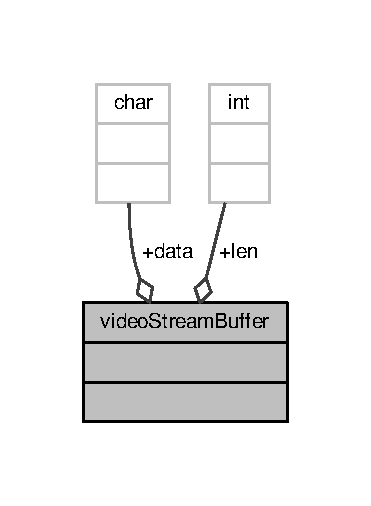
\includegraphics[width=178pt]{structvideoStreamBuffer__coll__graph}
\end{center}
\end{figure}
\subsection*{Public Attributes}
\begin{DoxyCompactItemize}
\item 
char $\ast$ \hyperlink{structvideoStreamBuffer_a2854e01e5c157423b0b8e84f3b264daa}{data}
\item 
int \hyperlink{structvideoStreamBuffer_a9c5bdf26c0bea4bb642eab19ef08213f}{len}
\end{DoxyCompactItemize}


\subsection{Member Data Documentation}
\index{video\+Stream\+Buffer@{video\+Stream\+Buffer}!data@{data}}
\index{data@{data}!video\+Stream\+Buffer@{video\+Stream\+Buffer}}
\subsubsection[{\texorpdfstring{data}{data}}]{\setlength{\rightskip}{0pt plus 5cm}char$\ast$ video\+Stream\+Buffer\+::data}\hypertarget{structvideoStreamBuffer_a2854e01e5c157423b0b8e84f3b264daa}{}\label{structvideoStreamBuffer_a2854e01e5c157423b0b8e84f3b264daa}
\index{video\+Stream\+Buffer@{video\+Stream\+Buffer}!len@{len}}
\index{len@{len}!video\+Stream\+Buffer@{video\+Stream\+Buffer}}
\subsubsection[{\texorpdfstring{len}{len}}]{\setlength{\rightskip}{0pt plus 5cm}int video\+Stream\+Buffer\+::len}\hypertarget{structvideoStreamBuffer_a9c5bdf26c0bea4bb642eab19ef08213f}{}\label{structvideoStreamBuffer_a9c5bdf26c0bea4bb642eab19ef08213f}


The documentation for this struct was generated from the following file\+:\begin{DoxyCompactItemize}
\item 
include/stream/\hyperlink{video-stream-stereo-device_8h}{video-\/stream-\/stereo-\/device.\+h}\end{DoxyCompactItemize}

\hypertarget{classVideoStreamStereoDevice}{}\section{Video\+Stream\+Stereo\+Device Class Reference}
\label{classVideoStreamStereoDevice}\index{Video\+Stream\+Stereo\+Device@{Video\+Stream\+Stereo\+Device}}


{\ttfamily \#include $<$video-\/stream-\/stereo-\/device.\+h$>$}



Inheritance diagram for Video\+Stream\+Stereo\+Device\+:
\nopagebreak
\begin{figure}[H]
\begin{center}
\leavevmode
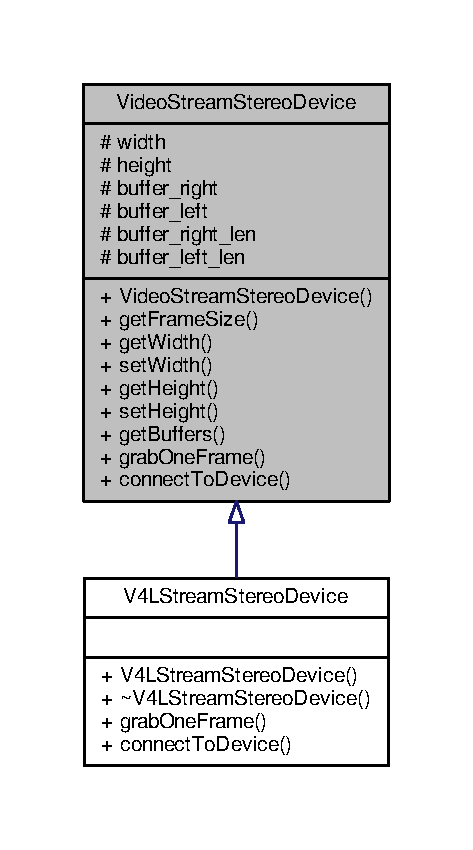
\includegraphics[width=227pt]{classVideoStreamStereoDevice__inherit__graph}
\end{center}
\end{figure}


Collaboration diagram for Video\+Stream\+Stereo\+Device\+:
\nopagebreak
\begin{figure}[H]
\begin{center}
\leavevmode
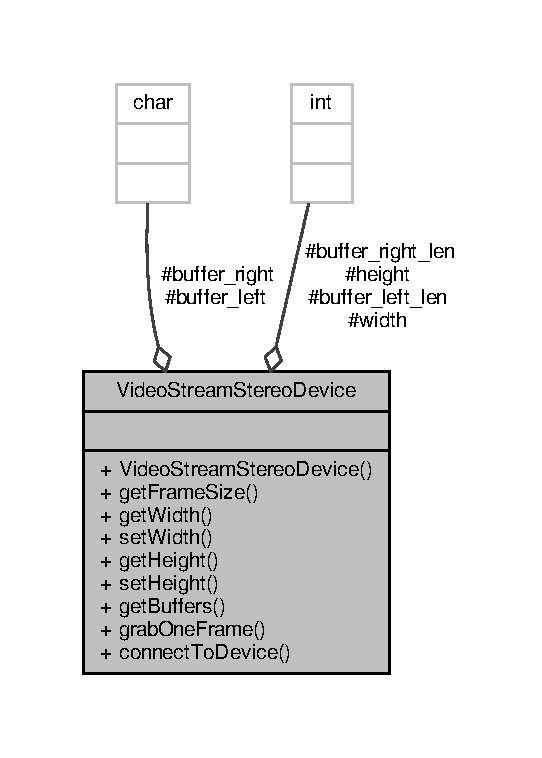
\includegraphics[width=260pt]{classVideoStreamStereoDevice__coll__graph}
\end{center}
\end{figure}
\subsection*{Public Member Functions}
\begin{DoxyCompactItemize}
\item 
\hyperlink{classVideoStreamStereoDevice_a6ff6603f94f44f7dac28de4ac195a18c}{Video\+Stream\+Stereo\+Device} ()
\item 
int \hyperlink{classVideoStreamStereoDevice_ab298f30a6339e8729d95b58fec0fdd42}{get\+Frame\+Size} () const 
\item 
int \hyperlink{classVideoStreamStereoDevice_a17527e897d16e363003d37c74b390e33}{get\+Width} () const 
\item 
void \hyperlink{classVideoStreamStereoDevice_a3104086b06532035588bb8d424f15738}{set\+Width} (int value)
\item 
int \hyperlink{classVideoStreamStereoDevice_aa0410bfdaf9467a24e4d25fdbe7062d8}{get\+Height} () const 
\item 
void \hyperlink{classVideoStreamStereoDevice_a536021533e1e4cb678338a961b095429}{set\+Height} (int value)
\item 
void \hyperlink{classVideoStreamStereoDevice_afee2d316610727d829ed75b7fe51a777}{get\+Buffers} (struct \hyperlink{structvideoStreamBuffer}{video\+Stream\+Buffer} $\ast$left, struct \hyperlink{structvideoStreamBuffer}{video\+Stream\+Buffer} $\ast$right)
\item 
virtual int \hyperlink{classVideoStreamStereoDevice_a98ac1bfc13c0d700ee8f4658485e0d39}{grab\+One\+Frame} ()=0
\item 
virtual int \hyperlink{classVideoStreamStereoDevice_aa85f8836979a061a7f11d0e3ca0f9c44}{connect\+To\+Device} ()=0
\end{DoxyCompactItemize}
\subsection*{Protected Attributes}
\begin{DoxyCompactItemize}
\item 
int \hyperlink{classVideoStreamStereoDevice_a87596748c13021a3623bb55de4c9be14}{width}
\item 
int \hyperlink{classVideoStreamStereoDevice_a97af0c098374ce089e71d9020b792f1f}{height}
\item 
char $\ast$ \hyperlink{classVideoStreamStereoDevice_a1d854ebc4900384b76163e1cd738cd98}{buffer\+\_\+right}
\item 
char $\ast$ \hyperlink{classVideoStreamStereoDevice_a80c9ca761c34011dc5dc90d629df3f15}{buffer\+\_\+left}
\item 
int \hyperlink{classVideoStreamStereoDevice_a7b8a59b76b5763b67cb357171c9396d7}{buffer\+\_\+right\+\_\+len}
\item 
int \hyperlink{classVideoStreamStereoDevice_a0ae10b0a0bc18b5f3899954c67347c61}{buffer\+\_\+left\+\_\+len}
\end{DoxyCompactItemize}


\subsection{Constructor \& Destructor Documentation}
\index{Video\+Stream\+Stereo\+Device@{Video\+Stream\+Stereo\+Device}!Video\+Stream\+Stereo\+Device@{Video\+Stream\+Stereo\+Device}}
\index{Video\+Stream\+Stereo\+Device@{Video\+Stream\+Stereo\+Device}!Video\+Stream\+Stereo\+Device@{Video\+Stream\+Stereo\+Device}}
\subsubsection[{\texorpdfstring{Video\+Stream\+Stereo\+Device()}{VideoStreamStereoDevice()}}]{\setlength{\rightskip}{0pt plus 5cm}Video\+Stream\+Stereo\+Device\+::\+Video\+Stream\+Stereo\+Device (
\begin{DoxyParamCaption}
{}
\end{DoxyParamCaption}
)\hspace{0.3cm}{\ttfamily [explicit]}}\hypertarget{classVideoStreamStereoDevice_a6ff6603f94f44f7dac28de4ac195a18c}{}\label{classVideoStreamStereoDevice_a6ff6603f94f44f7dac28de4ac195a18c}


\subsection{Member Function Documentation}
\index{Video\+Stream\+Stereo\+Device@{Video\+Stream\+Stereo\+Device}!connect\+To\+Device@{connect\+To\+Device}}
\index{connect\+To\+Device@{connect\+To\+Device}!Video\+Stream\+Stereo\+Device@{Video\+Stream\+Stereo\+Device}}
\subsubsection[{\texorpdfstring{connect\+To\+Device()=0}{connectToDevice()=0}}]{\setlength{\rightskip}{0pt plus 5cm}virtual int Video\+Stream\+Stereo\+Device\+::connect\+To\+Device (
\begin{DoxyParamCaption}
{}
\end{DoxyParamCaption}
)\hspace{0.3cm}{\ttfamily [pure virtual]}}\hypertarget{classVideoStreamStereoDevice_aa85f8836979a061a7f11d0e3ca0f9c44}{}\label{classVideoStreamStereoDevice_aa85f8836979a061a7f11d0e3ca0f9c44}


Implemented in \hyperlink{classV4LStreamStereoDevice_a0ecb2dd2636fcbfccc0e43604bf9bd14}{V4\+L\+Stream\+Stereo\+Device}.

\index{Video\+Stream\+Stereo\+Device@{Video\+Stream\+Stereo\+Device}!get\+Buffers@{get\+Buffers}}
\index{get\+Buffers@{get\+Buffers}!Video\+Stream\+Stereo\+Device@{Video\+Stream\+Stereo\+Device}}
\subsubsection[{\texorpdfstring{get\+Buffers(struct video\+Stream\+Buffer $\ast$left, struct video\+Stream\+Buffer $\ast$right)}{getBuffers(struct videoStreamBuffer *left, struct videoStreamBuffer *right)}}]{\setlength{\rightskip}{0pt plus 5cm}void Video\+Stream\+Stereo\+Device\+::get\+Buffers (
\begin{DoxyParamCaption}
\item[{struct {\bf video\+Stream\+Buffer} $\ast$}]{left, }
\item[{struct {\bf video\+Stream\+Buffer} $\ast$}]{right}
\end{DoxyParamCaption}
)}\hypertarget{classVideoStreamStereoDevice_afee2d316610727d829ed75b7fe51a777}{}\label{classVideoStreamStereoDevice_afee2d316610727d829ed75b7fe51a777}
\index{Video\+Stream\+Stereo\+Device@{Video\+Stream\+Stereo\+Device}!get\+Frame\+Size@{get\+Frame\+Size}}
\index{get\+Frame\+Size@{get\+Frame\+Size}!Video\+Stream\+Stereo\+Device@{Video\+Stream\+Stereo\+Device}}
\subsubsection[{\texorpdfstring{get\+Frame\+Size() const }{getFrameSize() const }}]{\setlength{\rightskip}{0pt plus 5cm}int Video\+Stream\+Stereo\+Device\+::get\+Frame\+Size (
\begin{DoxyParamCaption}
{}
\end{DoxyParamCaption}
) const}\hypertarget{classVideoStreamStereoDevice_ab298f30a6339e8729d95b58fec0fdd42}{}\label{classVideoStreamStereoDevice_ab298f30a6339e8729d95b58fec0fdd42}
\index{Video\+Stream\+Stereo\+Device@{Video\+Stream\+Stereo\+Device}!get\+Height@{get\+Height}}
\index{get\+Height@{get\+Height}!Video\+Stream\+Stereo\+Device@{Video\+Stream\+Stereo\+Device}}
\subsubsection[{\texorpdfstring{get\+Height() const }{getHeight() const }}]{\setlength{\rightskip}{0pt plus 5cm}int Video\+Stream\+Stereo\+Device\+::get\+Height (
\begin{DoxyParamCaption}
{}
\end{DoxyParamCaption}
) const}\hypertarget{classVideoStreamStereoDevice_aa0410bfdaf9467a24e4d25fdbe7062d8}{}\label{classVideoStreamStereoDevice_aa0410bfdaf9467a24e4d25fdbe7062d8}
\index{Video\+Stream\+Stereo\+Device@{Video\+Stream\+Stereo\+Device}!get\+Width@{get\+Width}}
\index{get\+Width@{get\+Width}!Video\+Stream\+Stereo\+Device@{Video\+Stream\+Stereo\+Device}}
\subsubsection[{\texorpdfstring{get\+Width() const }{getWidth() const }}]{\setlength{\rightskip}{0pt plus 5cm}int Video\+Stream\+Stereo\+Device\+::get\+Width (
\begin{DoxyParamCaption}
{}
\end{DoxyParamCaption}
) const}\hypertarget{classVideoStreamStereoDevice_a17527e897d16e363003d37c74b390e33}{}\label{classVideoStreamStereoDevice_a17527e897d16e363003d37c74b390e33}
\index{Video\+Stream\+Stereo\+Device@{Video\+Stream\+Stereo\+Device}!grab\+One\+Frame@{grab\+One\+Frame}}
\index{grab\+One\+Frame@{grab\+One\+Frame}!Video\+Stream\+Stereo\+Device@{Video\+Stream\+Stereo\+Device}}
\subsubsection[{\texorpdfstring{grab\+One\+Frame()=0}{grabOneFrame()=0}}]{\setlength{\rightskip}{0pt plus 5cm}virtual int Video\+Stream\+Stereo\+Device\+::grab\+One\+Frame (
\begin{DoxyParamCaption}
{}
\end{DoxyParamCaption}
)\hspace{0.3cm}{\ttfamily [pure virtual]}}\hypertarget{classVideoStreamStereoDevice_a98ac1bfc13c0d700ee8f4658485e0d39}{}\label{classVideoStreamStereoDevice_a98ac1bfc13c0d700ee8f4658485e0d39}


Implemented in \hyperlink{classV4LStreamStereoDevice_af5170cee3401eb70e771b56fbf2104d7}{V4\+L\+Stream\+Stereo\+Device}.

\index{Video\+Stream\+Stereo\+Device@{Video\+Stream\+Stereo\+Device}!set\+Height@{set\+Height}}
\index{set\+Height@{set\+Height}!Video\+Stream\+Stereo\+Device@{Video\+Stream\+Stereo\+Device}}
\subsubsection[{\texorpdfstring{set\+Height(int value)}{setHeight(int value)}}]{\setlength{\rightskip}{0pt plus 5cm}void Video\+Stream\+Stereo\+Device\+::set\+Height (
\begin{DoxyParamCaption}
\item[{int}]{value}
\end{DoxyParamCaption}
)}\hypertarget{classVideoStreamStereoDevice_a536021533e1e4cb678338a961b095429}{}\label{classVideoStreamStereoDevice_a536021533e1e4cb678338a961b095429}
\index{Video\+Stream\+Stereo\+Device@{Video\+Stream\+Stereo\+Device}!set\+Width@{set\+Width}}
\index{set\+Width@{set\+Width}!Video\+Stream\+Stereo\+Device@{Video\+Stream\+Stereo\+Device}}
\subsubsection[{\texorpdfstring{set\+Width(int value)}{setWidth(int value)}}]{\setlength{\rightskip}{0pt plus 5cm}void Video\+Stream\+Stereo\+Device\+::set\+Width (
\begin{DoxyParamCaption}
\item[{int}]{value}
\end{DoxyParamCaption}
)}\hypertarget{classVideoStreamStereoDevice_a3104086b06532035588bb8d424f15738}{}\label{classVideoStreamStereoDevice_a3104086b06532035588bb8d424f15738}


\subsection{Member Data Documentation}
\index{Video\+Stream\+Stereo\+Device@{Video\+Stream\+Stereo\+Device}!buffer\+\_\+left@{buffer\+\_\+left}}
\index{buffer\+\_\+left@{buffer\+\_\+left}!Video\+Stream\+Stereo\+Device@{Video\+Stream\+Stereo\+Device}}
\subsubsection[{\texorpdfstring{buffer\+\_\+left}{buffer_left}}]{\setlength{\rightskip}{0pt plus 5cm}char$\ast$ Video\+Stream\+Stereo\+Device\+::buffer\+\_\+left\hspace{0.3cm}{\ttfamily [protected]}}\hypertarget{classVideoStreamStereoDevice_a80c9ca761c34011dc5dc90d629df3f15}{}\label{classVideoStreamStereoDevice_a80c9ca761c34011dc5dc90d629df3f15}
\index{Video\+Stream\+Stereo\+Device@{Video\+Stream\+Stereo\+Device}!buffer\+\_\+left\+\_\+len@{buffer\+\_\+left\+\_\+len}}
\index{buffer\+\_\+left\+\_\+len@{buffer\+\_\+left\+\_\+len}!Video\+Stream\+Stereo\+Device@{Video\+Stream\+Stereo\+Device}}
\subsubsection[{\texorpdfstring{buffer\+\_\+left\+\_\+len}{buffer_left_len}}]{\setlength{\rightskip}{0pt plus 5cm}int Video\+Stream\+Stereo\+Device\+::buffer\+\_\+left\+\_\+len\hspace{0.3cm}{\ttfamily [protected]}}\hypertarget{classVideoStreamStereoDevice_a0ae10b0a0bc18b5f3899954c67347c61}{}\label{classVideoStreamStereoDevice_a0ae10b0a0bc18b5f3899954c67347c61}
\index{Video\+Stream\+Stereo\+Device@{Video\+Stream\+Stereo\+Device}!buffer\+\_\+right@{buffer\+\_\+right}}
\index{buffer\+\_\+right@{buffer\+\_\+right}!Video\+Stream\+Stereo\+Device@{Video\+Stream\+Stereo\+Device}}
\subsubsection[{\texorpdfstring{buffer\+\_\+right}{buffer_right}}]{\setlength{\rightskip}{0pt plus 5cm}char$\ast$ Video\+Stream\+Stereo\+Device\+::buffer\+\_\+right\hspace{0.3cm}{\ttfamily [protected]}}\hypertarget{classVideoStreamStereoDevice_a1d854ebc4900384b76163e1cd738cd98}{}\label{classVideoStreamStereoDevice_a1d854ebc4900384b76163e1cd738cd98}
\index{Video\+Stream\+Stereo\+Device@{Video\+Stream\+Stereo\+Device}!buffer\+\_\+right\+\_\+len@{buffer\+\_\+right\+\_\+len}}
\index{buffer\+\_\+right\+\_\+len@{buffer\+\_\+right\+\_\+len}!Video\+Stream\+Stereo\+Device@{Video\+Stream\+Stereo\+Device}}
\subsubsection[{\texorpdfstring{buffer\+\_\+right\+\_\+len}{buffer_right_len}}]{\setlength{\rightskip}{0pt plus 5cm}int Video\+Stream\+Stereo\+Device\+::buffer\+\_\+right\+\_\+len\hspace{0.3cm}{\ttfamily [protected]}}\hypertarget{classVideoStreamStereoDevice_a7b8a59b76b5763b67cb357171c9396d7}{}\label{classVideoStreamStereoDevice_a7b8a59b76b5763b67cb357171c9396d7}
\index{Video\+Stream\+Stereo\+Device@{Video\+Stream\+Stereo\+Device}!height@{height}}
\index{height@{height}!Video\+Stream\+Stereo\+Device@{Video\+Stream\+Stereo\+Device}}
\subsubsection[{\texorpdfstring{height}{height}}]{\setlength{\rightskip}{0pt plus 5cm}int Video\+Stream\+Stereo\+Device\+::height\hspace{0.3cm}{\ttfamily [protected]}}\hypertarget{classVideoStreamStereoDevice_a97af0c098374ce089e71d9020b792f1f}{}\label{classVideoStreamStereoDevice_a97af0c098374ce089e71d9020b792f1f}
\index{Video\+Stream\+Stereo\+Device@{Video\+Stream\+Stereo\+Device}!width@{width}}
\index{width@{width}!Video\+Stream\+Stereo\+Device@{Video\+Stream\+Stereo\+Device}}
\subsubsection[{\texorpdfstring{width}{width}}]{\setlength{\rightskip}{0pt plus 5cm}int Video\+Stream\+Stereo\+Device\+::width\hspace{0.3cm}{\ttfamily [protected]}}\hypertarget{classVideoStreamStereoDevice_a87596748c13021a3623bb55de4c9be14}{}\label{classVideoStreamStereoDevice_a87596748c13021a3623bb55de4c9be14}


The documentation for this class was generated from the following files\+:\begin{DoxyCompactItemize}
\item 
include/stream/\hyperlink{video-stream-stereo-device_8h}{video-\/stream-\/stereo-\/device.\+h}\item 
stream/\hyperlink{video-stream-stereo-device_8cpp}{video-\/stream-\/stereo-\/device.\+cpp}\end{DoxyCompactItemize}

\hypertarget{structxmorph__filter__uio__info}{}\section{xmorph\+\_\+filter\+\_\+uio\+\_\+info Struct Reference}
\label{structxmorph__filter__uio__info}\index{xmorph\+\_\+filter\+\_\+uio\+\_\+info@{xmorph\+\_\+filter\+\_\+uio\+\_\+info}}


{\ttfamily \#include $<$mf-\/hw-\/ip.\+h$>$}



Collaboration diagram for xmorph\+\_\+filter\+\_\+uio\+\_\+info\+:
\nopagebreak
\begin{figure}[H]
\begin{center}
\leavevmode
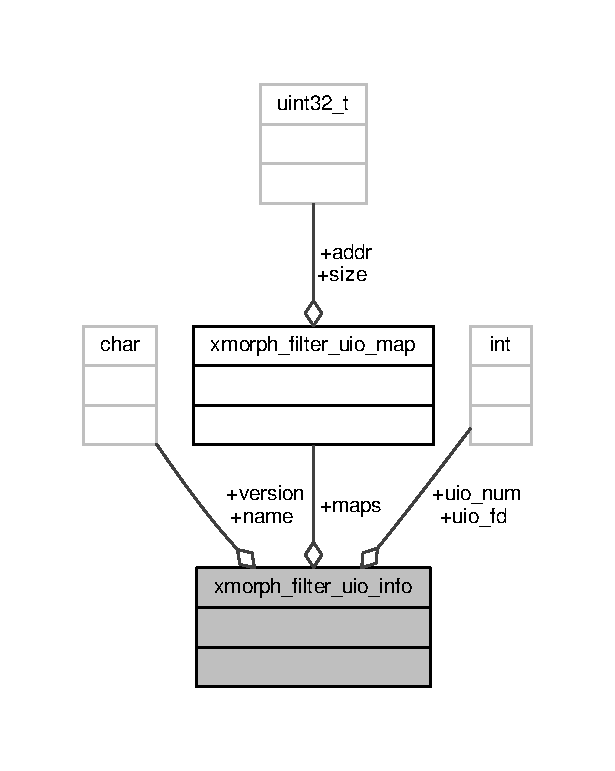
\includegraphics[width=295pt]{structxmorph__filter__uio__info__coll__graph}
\end{center}
\end{figure}
\subsection*{Public Attributes}
\begin{DoxyCompactItemize}
\item 
int \hyperlink{structxmorph__filter__uio__info_ac61f755f744e49006814f2a7542e80c6}{uio\+\_\+fd}
\item 
int \hyperlink{structxmorph__filter__uio__info_ad4f78bdfe803c26ef3801365c475d410}{uio\+\_\+num}
\item 
char \hyperlink{structxmorph__filter__uio__info_ad50f0ebca864e8164b94c25c79e36b28}{name} \mbox{[}\hyperlink{uio_8h_a5ed3f1c67d5551770a91ef53fe208c83}{M\+A\+X\+\_\+\+U\+I\+O\+\_\+\+N\+A\+M\+E\+\_\+\+S\+I\+ZE}\mbox{]}
\item 
char \hyperlink{structxmorph__filter__uio__info_af338637c0c32343f3cd6806949f1f822}{version} \mbox{[}\hyperlink{uio_8h_a5ed3f1c67d5551770a91ef53fe208c83}{M\+A\+X\+\_\+\+U\+I\+O\+\_\+\+N\+A\+M\+E\+\_\+\+S\+I\+ZE}\mbox{]}
\item 
\hyperlink{structxmorph__filter__uio__map}{xmorph\+\_\+filter\+\_\+uio\+\_\+map} \hyperlink{structxmorph__filter__uio__info_a4be1580d5c61c751dce585288b43a231}{maps} \mbox{[}\hyperlink{uio_8h_a05a77cb47b9d8cdaaee64df37627ffdc}{M\+A\+X\+\_\+\+U\+I\+O\+\_\+\+M\+A\+PS}\mbox{]}
\end{DoxyCompactItemize}


\subsection{Member Data Documentation}
\index{xmorph\+\_\+filter\+\_\+uio\+\_\+info@{xmorph\+\_\+filter\+\_\+uio\+\_\+info}!maps@{maps}}
\index{maps@{maps}!xmorph\+\_\+filter\+\_\+uio\+\_\+info@{xmorph\+\_\+filter\+\_\+uio\+\_\+info}}
\subsubsection[{\texorpdfstring{maps}{maps}}]{\setlength{\rightskip}{0pt plus 5cm}{\bf xmorph\+\_\+filter\+\_\+uio\+\_\+map} xmorph\+\_\+filter\+\_\+uio\+\_\+info\+::maps\mbox{[}{\bf M\+A\+X\+\_\+\+U\+I\+O\+\_\+\+M\+A\+PS}\mbox{]}}\hypertarget{structxmorph__filter__uio__info_a4be1580d5c61c751dce585288b43a231}{}\label{structxmorph__filter__uio__info_a4be1580d5c61c751dce585288b43a231}
\index{xmorph\+\_\+filter\+\_\+uio\+\_\+info@{xmorph\+\_\+filter\+\_\+uio\+\_\+info}!name@{name}}
\index{name@{name}!xmorph\+\_\+filter\+\_\+uio\+\_\+info@{xmorph\+\_\+filter\+\_\+uio\+\_\+info}}
\subsubsection[{\texorpdfstring{name}{name}}]{\setlength{\rightskip}{0pt plus 5cm}char xmorph\+\_\+filter\+\_\+uio\+\_\+info\+::name\mbox{[}{\bf M\+A\+X\+\_\+\+U\+I\+O\+\_\+\+N\+A\+M\+E\+\_\+\+S\+I\+ZE}\mbox{]}}\hypertarget{structxmorph__filter__uio__info_ad50f0ebca864e8164b94c25c79e36b28}{}\label{structxmorph__filter__uio__info_ad50f0ebca864e8164b94c25c79e36b28}
\index{xmorph\+\_\+filter\+\_\+uio\+\_\+info@{xmorph\+\_\+filter\+\_\+uio\+\_\+info}!uio\+\_\+fd@{uio\+\_\+fd}}
\index{uio\+\_\+fd@{uio\+\_\+fd}!xmorph\+\_\+filter\+\_\+uio\+\_\+info@{xmorph\+\_\+filter\+\_\+uio\+\_\+info}}
\subsubsection[{\texorpdfstring{uio\+\_\+fd}{uio_fd}}]{\setlength{\rightskip}{0pt plus 5cm}int xmorph\+\_\+filter\+\_\+uio\+\_\+info\+::uio\+\_\+fd}\hypertarget{structxmorph__filter__uio__info_ac61f755f744e49006814f2a7542e80c6}{}\label{structxmorph__filter__uio__info_ac61f755f744e49006814f2a7542e80c6}
\index{xmorph\+\_\+filter\+\_\+uio\+\_\+info@{xmorph\+\_\+filter\+\_\+uio\+\_\+info}!uio\+\_\+num@{uio\+\_\+num}}
\index{uio\+\_\+num@{uio\+\_\+num}!xmorph\+\_\+filter\+\_\+uio\+\_\+info@{xmorph\+\_\+filter\+\_\+uio\+\_\+info}}
\subsubsection[{\texorpdfstring{uio\+\_\+num}{uio_num}}]{\setlength{\rightskip}{0pt plus 5cm}int xmorph\+\_\+filter\+\_\+uio\+\_\+info\+::uio\+\_\+num}\hypertarget{structxmorph__filter__uio__info_ad4f78bdfe803c26ef3801365c475d410}{}\label{structxmorph__filter__uio__info_ad4f78bdfe803c26ef3801365c475d410}
\index{xmorph\+\_\+filter\+\_\+uio\+\_\+info@{xmorph\+\_\+filter\+\_\+uio\+\_\+info}!version@{version}}
\index{version@{version}!xmorph\+\_\+filter\+\_\+uio\+\_\+info@{xmorph\+\_\+filter\+\_\+uio\+\_\+info}}
\subsubsection[{\texorpdfstring{version}{version}}]{\setlength{\rightskip}{0pt plus 5cm}char xmorph\+\_\+filter\+\_\+uio\+\_\+info\+::version\mbox{[}{\bf M\+A\+X\+\_\+\+U\+I\+O\+\_\+\+N\+A\+M\+E\+\_\+\+S\+I\+ZE}\mbox{]}}\hypertarget{structxmorph__filter__uio__info_af338637c0c32343f3cd6806949f1f822}{}\label{structxmorph__filter__uio__info_af338637c0c32343f3cd6806949f1f822}


The documentation for this struct was generated from the following file\+:\begin{DoxyCompactItemize}
\item 
include/filter/\hyperlink{mf-hw-ip_8h}{mf-\/hw-\/ip.\+h}\end{DoxyCompactItemize}

\hypertarget{structxmorph__filter__uio__map}{}\section{xmorph\+\_\+filter\+\_\+uio\+\_\+map Struct Reference}
\label{structxmorph__filter__uio__map}\index{xmorph\+\_\+filter\+\_\+uio\+\_\+map@{xmorph\+\_\+filter\+\_\+uio\+\_\+map}}


{\ttfamily \#include $<$mf-\/hw-\/ip.\+h$>$}



Collaboration diagram for xmorph\+\_\+filter\+\_\+uio\+\_\+map\+:
\nopagebreak
\begin{figure}[H]
\begin{center}
\leavevmode
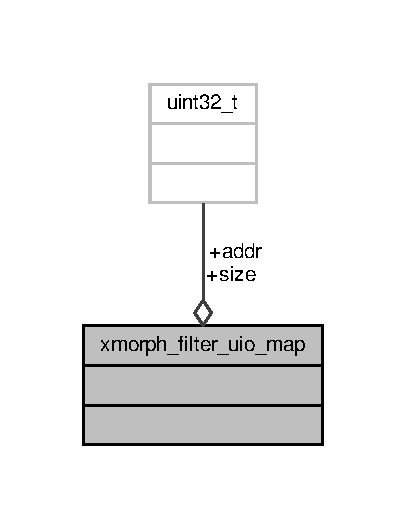
\includegraphics[width=195pt]{structxmorph__filter__uio__map__coll__graph}
\end{center}
\end{figure}
\subsection*{Public Attributes}
\begin{DoxyCompactItemize}
\item 
uint32\+\_\+t \hyperlink{structxmorph__filter__uio__map_afc5d71f297427642921e2bdc1650db31}{addr}
\item 
uint32\+\_\+t \hyperlink{structxmorph__filter__uio__map_a5da76368d6196b966516005fdae05937}{size}
\end{DoxyCompactItemize}


\subsection{Member Data Documentation}
\index{xmorph\+\_\+filter\+\_\+uio\+\_\+map@{xmorph\+\_\+filter\+\_\+uio\+\_\+map}!addr@{addr}}
\index{addr@{addr}!xmorph\+\_\+filter\+\_\+uio\+\_\+map@{xmorph\+\_\+filter\+\_\+uio\+\_\+map}}
\subsubsection[{\texorpdfstring{addr}{addr}}]{\setlength{\rightskip}{0pt plus 5cm}uint32\+\_\+t xmorph\+\_\+filter\+\_\+uio\+\_\+map\+::addr}\hypertarget{structxmorph__filter__uio__map_afc5d71f297427642921e2bdc1650db31}{}\label{structxmorph__filter__uio__map_afc5d71f297427642921e2bdc1650db31}
\index{xmorph\+\_\+filter\+\_\+uio\+\_\+map@{xmorph\+\_\+filter\+\_\+uio\+\_\+map}!size@{size}}
\index{size@{size}!xmorph\+\_\+filter\+\_\+uio\+\_\+map@{xmorph\+\_\+filter\+\_\+uio\+\_\+map}}
\subsubsection[{\texorpdfstring{size}{size}}]{\setlength{\rightskip}{0pt plus 5cm}uint32\+\_\+t xmorph\+\_\+filter\+\_\+uio\+\_\+map\+::size}\hypertarget{structxmorph__filter__uio__map_a5da76368d6196b966516005fdae05937}{}\label{structxmorph__filter__uio__map_a5da76368d6196b966516005fdae05937}


The documentation for this struct was generated from the following file\+:\begin{DoxyCompactItemize}
\item 
include/filter/\hyperlink{mf-hw-ip_8h}{mf-\/hw-\/ip.\+h}\end{DoxyCompactItemize}

\chapter{File Documentation}
\hypertarget{decoder_8cpp}{}\section{decoder/decoder.cpp File Reference}
\label{decoder_8cpp}\index{decoder/decoder.\+cpp@{decoder/decoder.\+cpp}}
{\ttfamily \#include \char`\"{}decoder/decoder.\+h\char`\"{}}\\*
Include dependency graph for decoder.\+cpp\+:
\nopagebreak
\begin{figure}[H]
\begin{center}
\leavevmode
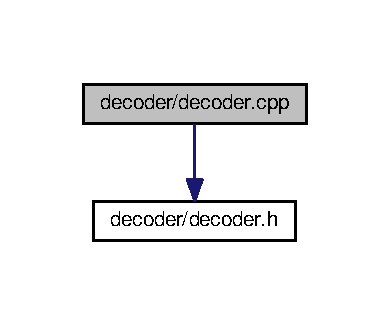
\includegraphics[width=187pt]{decoder_8cpp__incl}
\end{center}
\end{figure}

\hypertarget{mjpeg-decoder-sw_8cpp}{}\section{decoder/mjpeg-\/decoder-\/sw.cpp File Reference}
\label{mjpeg-decoder-sw_8cpp}\index{decoder/mjpeg-\/decoder-\/sw.\+cpp@{decoder/mjpeg-\/decoder-\/sw.\+cpp}}
{\ttfamily \#include \char`\"{}decoder/mjpeg-\/decoder-\/sw.\+h\char`\"{}}\\*
Include dependency graph for mjpeg-\/decoder-\/sw.cpp\+:
\nopagebreak
\begin{figure}[H]
\begin{center}
\leavevmode
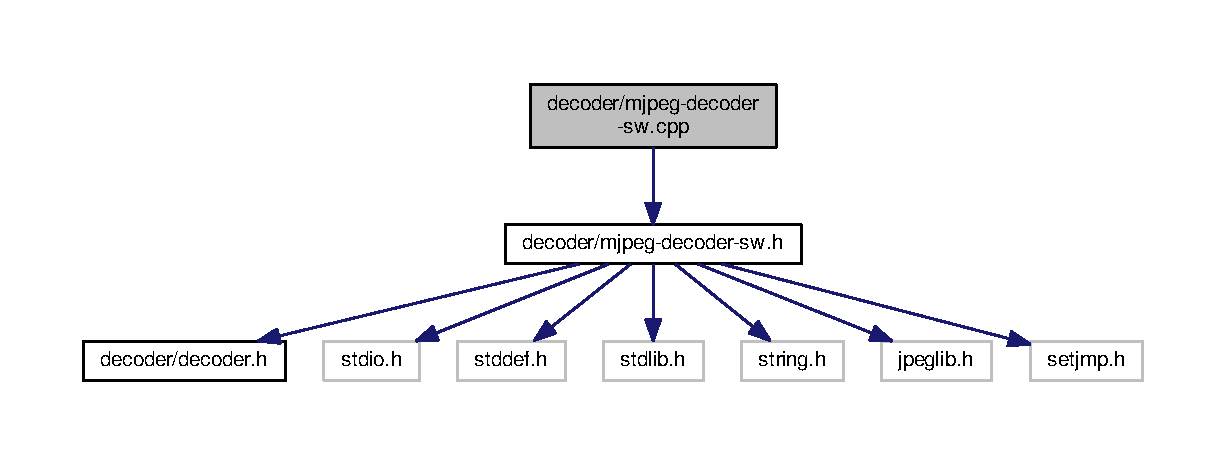
\includegraphics[width=350pt]{mjpeg-decoder-sw_8cpp__incl}
\end{center}
\end{figure}
\subsection*{Classes}
\begin{DoxyCompactItemize}
\item 
struct \hyperlink{structerror__mgr}{error\+\_\+mgr}
\end{DoxyCompactItemize}
\subsection*{Macros}
\begin{DoxyCompactItemize}
\item 
\#define \hyperlink{mjpeg-decoder-sw_8cpp_a3b7d514bed96e59bd95921d36f7b596c}{C\+O\+P\+Y\+\_\+\+H\+U\+F\+F\+\_\+\+T\+A\+B\+LE}(dinfo,  tbl,  name)
\end{DoxyCompactItemize}


\subsection{Macro Definition Documentation}
\index{mjpeg-\/decoder-\/sw.\+cpp@{mjpeg-\/decoder-\/sw.\+cpp}!C\+O\+P\+Y\+\_\+\+H\+U\+F\+F\+\_\+\+T\+A\+B\+LE@{C\+O\+P\+Y\+\_\+\+H\+U\+F\+F\+\_\+\+T\+A\+B\+LE}}
\index{C\+O\+P\+Y\+\_\+\+H\+U\+F\+F\+\_\+\+T\+A\+B\+LE@{C\+O\+P\+Y\+\_\+\+H\+U\+F\+F\+\_\+\+T\+A\+B\+LE}!mjpeg-\/decoder-\/sw.\+cpp@{mjpeg-\/decoder-\/sw.\+cpp}}
\subsubsection[{\texorpdfstring{C\+O\+P\+Y\+\_\+\+H\+U\+F\+F\+\_\+\+T\+A\+B\+LE}{COPY_HUFF_TABLE}}]{\setlength{\rightskip}{0pt plus 5cm}\#define C\+O\+P\+Y\+\_\+\+H\+U\+F\+F\+\_\+\+T\+A\+B\+LE(
\begin{DoxyParamCaption}
\item[{}]{dinfo, }
\item[{}]{tbl, }
\item[{}]{name}
\end{DoxyParamCaption}
)}\hypertarget{mjpeg-decoder-sw_8cpp_a3b7d514bed96e59bd95921d36f7b596c}{}\label{mjpeg-decoder-sw_8cpp_a3b7d514bed96e59bd95921d36f7b596c}
{\bfseries Value\+:}
\begin{DoxyCode}
\textcolor{keywordflow}{do} \{ \(\backslash\)
  if(dinfo->tbl == NULL) dinfo->tbl = jpeg\_alloc\_huff\_table((j\_common\_ptr)dinfo); \(\backslash\)
  memcpy(dinfo->tbl->bits, name\textcolor{preprocessor}{##\_len, sizeof(name##\_len)); \(\backslash\)}
\textcolor{preprocessor}{  memset(dinfo->tbl->huffval, 0, sizeof(dinfo->tbl->huffval)); \(\backslash\)}
\textcolor{preprocessor}{  memcpy(dinfo->tbl->huffval, name##\_val, sizeof(name##\_val)); \(\backslash\)}
\textcolor{preprocessor}{\} while(0)}
\end{DoxyCode}

\hypertarget{estimator_8cpp}{}\section{estimator.\+cpp File Reference}
\label{estimator_8cpp}\index{estimator.\+cpp@{estimator.\+cpp}}
{\ttfamily \#include \char`\"{}estimator.\+h\char`\"{}}\\*
Include dependency graph for estimator.\+cpp\+:
\nopagebreak
\begin{figure}[H]
\begin{center}
\leavevmode
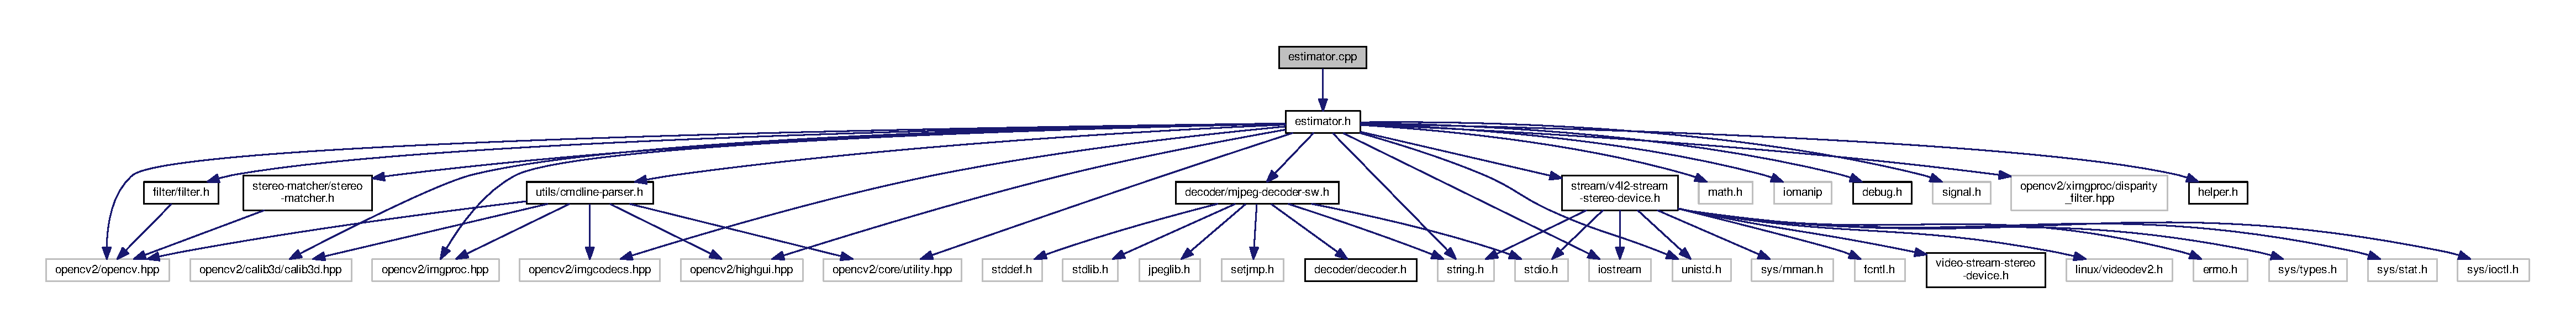
\includegraphics[width=350pt]{estimator_8cpp__incl}
\end{center}
\end{figure}

\hypertarget{filter_8cpp}{}\section{filter/filter.cpp File Reference}
\label{filter_8cpp}\index{filter/filter.\+cpp@{filter/filter.\+cpp}}
{\ttfamily \#include \char`\"{}filter/filter.\+h\char`\"{}}\\*
Include dependency graph for filter.\+cpp\+:
\nopagebreak
\begin{figure}[H]
\begin{center}
\leavevmode
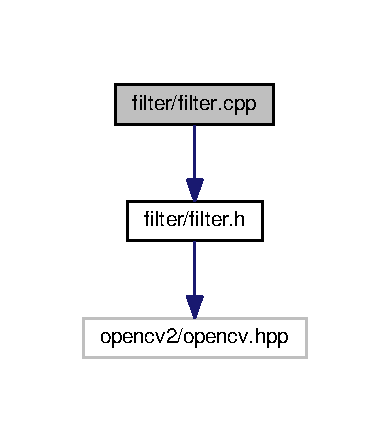
\includegraphics[width=187pt]{filter_8cpp__incl}
\end{center}
\end{figure}

\hypertarget{mf-hw-ip_8cpp}{}\section{filter/mf-\/hw-\/ip.cpp File Reference}
\label{mf-hw-ip_8cpp}\index{filter/mf-\/hw-\/ip.\+cpp@{filter/mf-\/hw-\/ip.\+cpp}}
{\ttfamily \#include \char`\"{}filter/mf-\/hw-\/ip.\+h\char`\"{}}\\*
Include dependency graph for mf-\/hw-\/ip.cpp\+:
\nopagebreak
\begin{figure}[H]
\begin{center}
\leavevmode
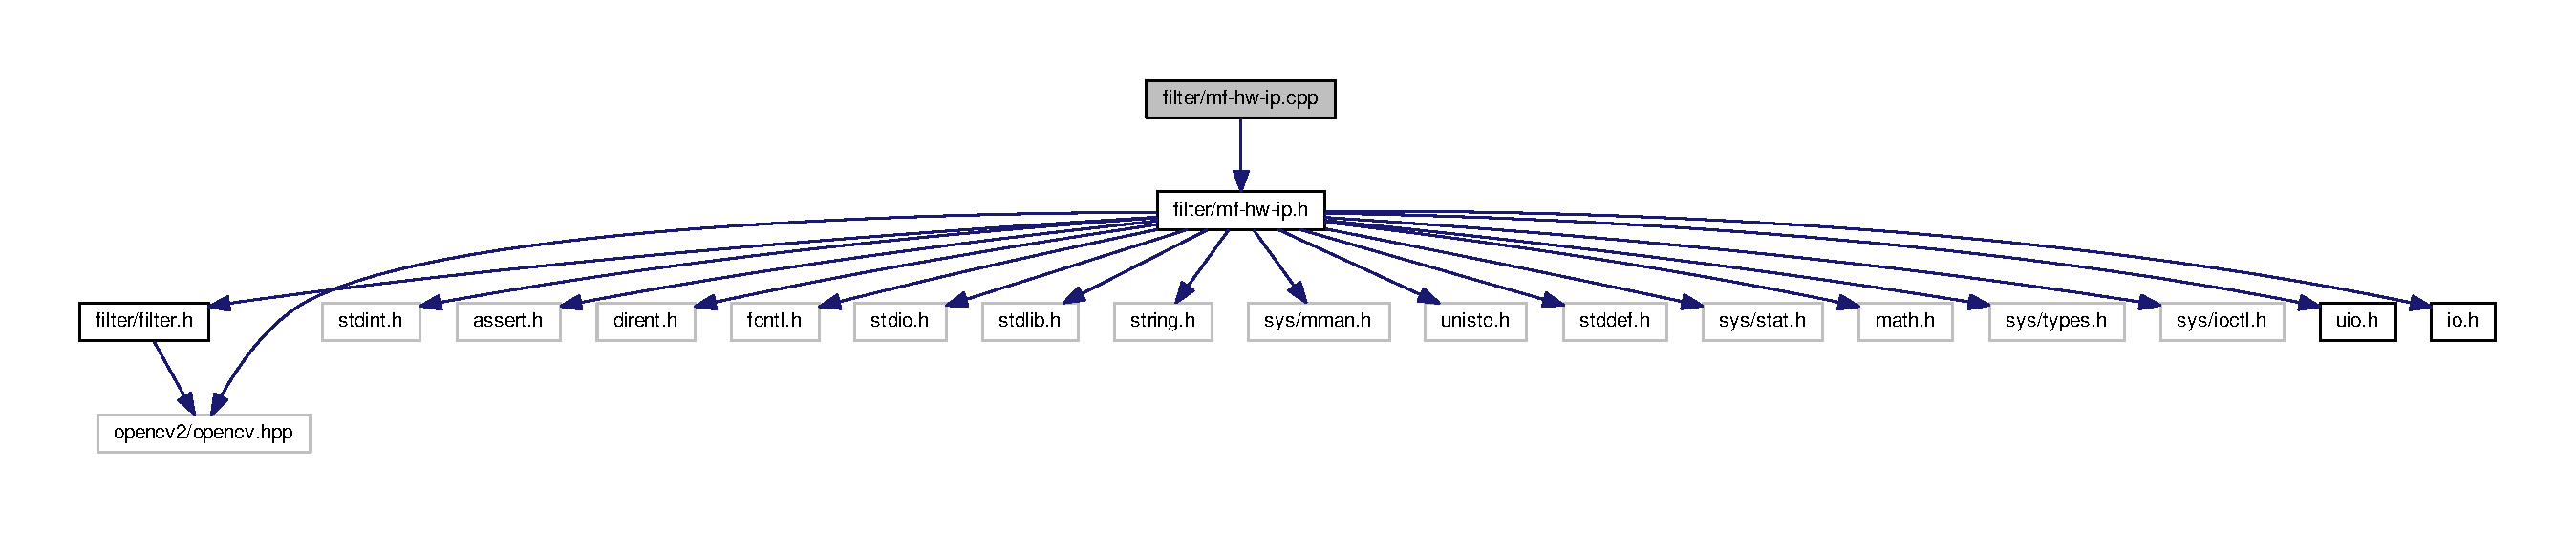
\includegraphics[width=350pt]{mf-hw-ip_8cpp__incl}
\end{center}
\end{figure}
\subsection*{Macros}
\begin{DoxyCompactItemize}
\item 
\#define \hyperlink{mf-hw-ip_8cpp_a525dc690f9b3aa98bfd8582d1834c592}{X\+M\+O\+R\+P\+H\+\_\+\+F\+I\+L\+T\+E\+R\+\_\+\+M\+A\+J\+OR}~10
\item 
\#define \hyperlink{mf-hw-ip_8cpp_a946c0d3be28eea0aa395341d5edad23b}{X\+M\+O\+R\+P\+H\+\_\+\+F\+I\+L\+T\+E\+R\+\_\+\+M\+I\+N\+OR}~235
\item 
\#define \hyperlink{mf-hw-ip_8cpp_a98531e30a77186fa74d7dd16ab7b4763}{X\+M\+O\+R\+P\+H\+\_\+\+I\+O\+C\+T\+L\+\_\+\+B\+A\+SE}~\textquotesingle{}S\textquotesingle{}
\item 
\#define \hyperlink{mf-hw-ip_8cpp_a9a30fd1ea7ebb580f4ffef098336f73f}{X\+M\+O\+R\+P\+H\+\_\+\+S\+T\+A\+RT}~\+\_\+\+IO(\hyperlink{mf-hw-ip_8cpp_a98531e30a77186fa74d7dd16ab7b4763}{X\+M\+O\+R\+P\+H\+\_\+\+I\+O\+C\+T\+L\+\_\+\+B\+A\+SE}, 0)
\item 
\#define \hyperlink{mf-hw-ip_8cpp_a1048583f6fc600a2b3b2c86b4b569a98}{X\+M\+O\+R\+P\+H\+\_\+\+S\+T\+OP}~\+\_\+\+IO(\hyperlink{mf-hw-ip_8cpp_a98531e30a77186fa74d7dd16ab7b4763}{X\+M\+O\+R\+P\+H\+\_\+\+I\+O\+C\+T\+L\+\_\+\+B\+A\+SE}, 1)
\item 
\#define \hyperlink{mf-hw-ip_8cpp_ad188c24482b068bac7d3dc2bb106bbfb}{X\+M\+O\+R\+P\+H\+\_\+\+S\+E\+T\+\_\+\+D\+IM}~\+\_\+\+IO(\hyperlink{mf-hw-ip_8cpp_a98531e30a77186fa74d7dd16ab7b4763}{X\+M\+O\+R\+P\+H\+\_\+\+I\+O\+C\+T\+L\+\_\+\+B\+A\+SE}, 2)
\end{DoxyCompactItemize}


\subsection{Macro Definition Documentation}
\index{mf-\/hw-\/ip.\+cpp@{mf-\/hw-\/ip.\+cpp}!X\+M\+O\+R\+P\+H\+\_\+\+F\+I\+L\+T\+E\+R\+\_\+\+M\+A\+J\+OR@{X\+M\+O\+R\+P\+H\+\_\+\+F\+I\+L\+T\+E\+R\+\_\+\+M\+A\+J\+OR}}
\index{X\+M\+O\+R\+P\+H\+\_\+\+F\+I\+L\+T\+E\+R\+\_\+\+M\+A\+J\+OR@{X\+M\+O\+R\+P\+H\+\_\+\+F\+I\+L\+T\+E\+R\+\_\+\+M\+A\+J\+OR}!mf-\/hw-\/ip.\+cpp@{mf-\/hw-\/ip.\+cpp}}
\subsubsection[{\texorpdfstring{X\+M\+O\+R\+P\+H\+\_\+\+F\+I\+L\+T\+E\+R\+\_\+\+M\+A\+J\+OR}{XMORPH_FILTER_MAJOR}}]{\setlength{\rightskip}{0pt plus 5cm}\#define X\+M\+O\+R\+P\+H\+\_\+\+F\+I\+L\+T\+E\+R\+\_\+\+M\+A\+J\+OR~10}\hypertarget{mf-hw-ip_8cpp_a525dc690f9b3aa98bfd8582d1834c592}{}\label{mf-hw-ip_8cpp_a525dc690f9b3aa98bfd8582d1834c592}
\index{mf-\/hw-\/ip.\+cpp@{mf-\/hw-\/ip.\+cpp}!X\+M\+O\+R\+P\+H\+\_\+\+F\+I\+L\+T\+E\+R\+\_\+\+M\+I\+N\+OR@{X\+M\+O\+R\+P\+H\+\_\+\+F\+I\+L\+T\+E\+R\+\_\+\+M\+I\+N\+OR}}
\index{X\+M\+O\+R\+P\+H\+\_\+\+F\+I\+L\+T\+E\+R\+\_\+\+M\+I\+N\+OR@{X\+M\+O\+R\+P\+H\+\_\+\+F\+I\+L\+T\+E\+R\+\_\+\+M\+I\+N\+OR}!mf-\/hw-\/ip.\+cpp@{mf-\/hw-\/ip.\+cpp}}
\subsubsection[{\texorpdfstring{X\+M\+O\+R\+P\+H\+\_\+\+F\+I\+L\+T\+E\+R\+\_\+\+M\+I\+N\+OR}{XMORPH_FILTER_MINOR}}]{\setlength{\rightskip}{0pt plus 5cm}\#define X\+M\+O\+R\+P\+H\+\_\+\+F\+I\+L\+T\+E\+R\+\_\+\+M\+I\+N\+OR~235}\hypertarget{mf-hw-ip_8cpp_a946c0d3be28eea0aa395341d5edad23b}{}\label{mf-hw-ip_8cpp_a946c0d3be28eea0aa395341d5edad23b}
\index{mf-\/hw-\/ip.\+cpp@{mf-\/hw-\/ip.\+cpp}!X\+M\+O\+R\+P\+H\+\_\+\+I\+O\+C\+T\+L\+\_\+\+B\+A\+SE@{X\+M\+O\+R\+P\+H\+\_\+\+I\+O\+C\+T\+L\+\_\+\+B\+A\+SE}}
\index{X\+M\+O\+R\+P\+H\+\_\+\+I\+O\+C\+T\+L\+\_\+\+B\+A\+SE@{X\+M\+O\+R\+P\+H\+\_\+\+I\+O\+C\+T\+L\+\_\+\+B\+A\+SE}!mf-\/hw-\/ip.\+cpp@{mf-\/hw-\/ip.\+cpp}}
\subsubsection[{\texorpdfstring{X\+M\+O\+R\+P\+H\+\_\+\+I\+O\+C\+T\+L\+\_\+\+B\+A\+SE}{XMORPH_IOCTL_BASE}}]{\setlength{\rightskip}{0pt plus 5cm}\#define X\+M\+O\+R\+P\+H\+\_\+\+I\+O\+C\+T\+L\+\_\+\+B\+A\+SE~\textquotesingle{}S\textquotesingle{}}\hypertarget{mf-hw-ip_8cpp_a98531e30a77186fa74d7dd16ab7b4763}{}\label{mf-hw-ip_8cpp_a98531e30a77186fa74d7dd16ab7b4763}
\index{mf-\/hw-\/ip.\+cpp@{mf-\/hw-\/ip.\+cpp}!X\+M\+O\+R\+P\+H\+\_\+\+S\+E\+T\+\_\+\+D\+IM@{X\+M\+O\+R\+P\+H\+\_\+\+S\+E\+T\+\_\+\+D\+IM}}
\index{X\+M\+O\+R\+P\+H\+\_\+\+S\+E\+T\+\_\+\+D\+IM@{X\+M\+O\+R\+P\+H\+\_\+\+S\+E\+T\+\_\+\+D\+IM}!mf-\/hw-\/ip.\+cpp@{mf-\/hw-\/ip.\+cpp}}
\subsubsection[{\texorpdfstring{X\+M\+O\+R\+P\+H\+\_\+\+S\+E\+T\+\_\+\+D\+IM}{XMORPH_SET_DIM}}]{\setlength{\rightskip}{0pt plus 5cm}\#define X\+M\+O\+R\+P\+H\+\_\+\+S\+E\+T\+\_\+\+D\+IM~\+\_\+\+IO({\bf X\+M\+O\+R\+P\+H\+\_\+\+I\+O\+C\+T\+L\+\_\+\+B\+A\+SE}, 2)}\hypertarget{mf-hw-ip_8cpp_ad188c24482b068bac7d3dc2bb106bbfb}{}\label{mf-hw-ip_8cpp_ad188c24482b068bac7d3dc2bb106bbfb}
\index{mf-\/hw-\/ip.\+cpp@{mf-\/hw-\/ip.\+cpp}!X\+M\+O\+R\+P\+H\+\_\+\+S\+T\+A\+RT@{X\+M\+O\+R\+P\+H\+\_\+\+S\+T\+A\+RT}}
\index{X\+M\+O\+R\+P\+H\+\_\+\+S\+T\+A\+RT@{X\+M\+O\+R\+P\+H\+\_\+\+S\+T\+A\+RT}!mf-\/hw-\/ip.\+cpp@{mf-\/hw-\/ip.\+cpp}}
\subsubsection[{\texorpdfstring{X\+M\+O\+R\+P\+H\+\_\+\+S\+T\+A\+RT}{XMORPH_START}}]{\setlength{\rightskip}{0pt plus 5cm}\#define X\+M\+O\+R\+P\+H\+\_\+\+S\+T\+A\+RT~\+\_\+\+IO({\bf X\+M\+O\+R\+P\+H\+\_\+\+I\+O\+C\+T\+L\+\_\+\+B\+A\+SE}, 0)}\hypertarget{mf-hw-ip_8cpp_a9a30fd1ea7ebb580f4ffef098336f73f}{}\label{mf-hw-ip_8cpp_a9a30fd1ea7ebb580f4ffef098336f73f}
\index{mf-\/hw-\/ip.\+cpp@{mf-\/hw-\/ip.\+cpp}!X\+M\+O\+R\+P\+H\+\_\+\+S\+T\+OP@{X\+M\+O\+R\+P\+H\+\_\+\+S\+T\+OP}}
\index{X\+M\+O\+R\+P\+H\+\_\+\+S\+T\+OP@{X\+M\+O\+R\+P\+H\+\_\+\+S\+T\+OP}!mf-\/hw-\/ip.\+cpp@{mf-\/hw-\/ip.\+cpp}}
\subsubsection[{\texorpdfstring{X\+M\+O\+R\+P\+H\+\_\+\+S\+T\+OP}{XMORPH_STOP}}]{\setlength{\rightskip}{0pt plus 5cm}\#define X\+M\+O\+R\+P\+H\+\_\+\+S\+T\+OP~\+\_\+\+IO({\bf X\+M\+O\+R\+P\+H\+\_\+\+I\+O\+C\+T\+L\+\_\+\+B\+A\+SE}, 1)}\hypertarget{mf-hw-ip_8cpp_a1048583f6fc600a2b3b2c86b4b569a98}{}\label{mf-hw-ip_8cpp_a1048583f6fc600a2b3b2c86b4b569a98}

\hypertarget{mf-sw_8cpp}{}\section{filter/mf-\/sw.cpp File Reference}
\label{mf-sw_8cpp}\index{filter/mf-\/sw.\+cpp@{filter/mf-\/sw.\+cpp}}
{\ttfamily \#include \char`\"{}filter/mf-\/sw.\+h\char`\"{}}\\*
Include dependency graph for mf-\/sw.cpp\+:
\nopagebreak
\begin{figure}[H]
\begin{center}
\leavevmode
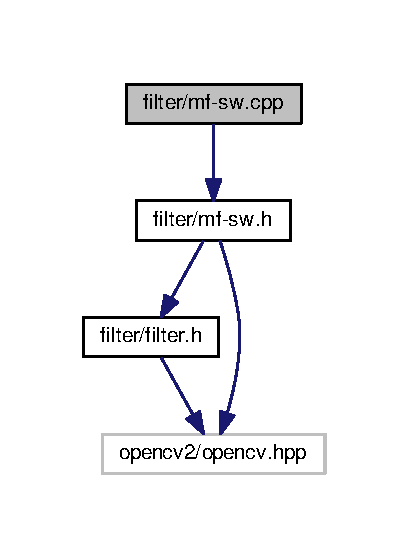
\includegraphics[width=196pt]{mf-sw_8cpp__incl}
\end{center}
\end{figure}

\hypertarget{debug_8h}{}\section{include/debug.h File Reference}
\label{debug_8h}\index{include/debug.\+h@{include/debug.\+h}}
This graph shows which files directly or indirectly include this file\+:
\nopagebreak
\begin{figure}[H]
\begin{center}
\leavevmode
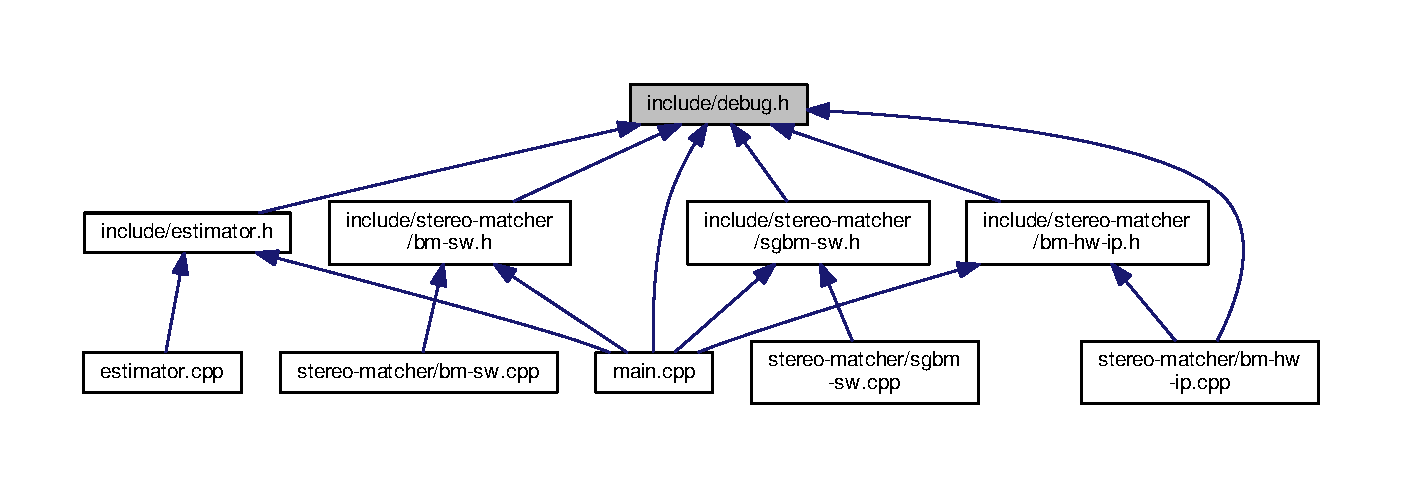
\includegraphics[width=350pt]{debug_8h__dep__incl}
\end{center}
\end{figure}
\subsection*{Macros}
\begin{DoxyCompactItemize}
\item 
\#define \hyperlink{debug_8h_ad72dbcf6d0153db1b8d8a58001feed83}{D\+E\+B\+UG}
\item 
\#define \hyperlink{debug_8h_a20f8a31603d3b132bf448a96fceec17d}{debug}(fmt, ...)~printf(fmt, \#\#\+\_\+\+\_\+\+V\+A\+\_\+\+A\+R\+G\+S\+\_\+\+\_\+)
\end{DoxyCompactItemize}


\subsection{Macro Definition Documentation}
\index{debug.\+h@{debug.\+h}!D\+E\+B\+UG@{D\+E\+B\+UG}}
\index{D\+E\+B\+UG@{D\+E\+B\+UG}!debug.\+h@{debug.\+h}}
\subsubsection[{\texorpdfstring{D\+E\+B\+UG}{DEBUG}}]{\setlength{\rightskip}{0pt plus 5cm}\#define D\+E\+B\+UG}\hypertarget{debug_8h_ad72dbcf6d0153db1b8d8a58001feed83}{}\label{debug_8h_ad72dbcf6d0153db1b8d8a58001feed83}
\index{debug.\+h@{debug.\+h}!debug@{debug}}
\index{debug@{debug}!debug.\+h@{debug.\+h}}
\subsubsection[{\texorpdfstring{debug}{debug}}]{\setlength{\rightskip}{0pt plus 5cm}\#define debug(
\begin{DoxyParamCaption}
\item[{}]{fmt, }
\item[{}]{...}
\end{DoxyParamCaption}
)~printf(fmt, \#\#\+\_\+\+\_\+\+V\+A\+\_\+\+A\+R\+G\+S\+\_\+\+\_\+)}\hypertarget{debug_8h_a20f8a31603d3b132bf448a96fceec17d}{}\label{debug_8h_a20f8a31603d3b132bf448a96fceec17d}

\hypertarget{decoder_8h}{}\section{include/decoder/decoder.h File Reference}
\label{decoder_8h}\index{include/decoder/decoder.\+h@{include/decoder/decoder.\+h}}
This graph shows which files directly or indirectly include this file\+:
\nopagebreak
\begin{figure}[H]
\begin{center}
\leavevmode
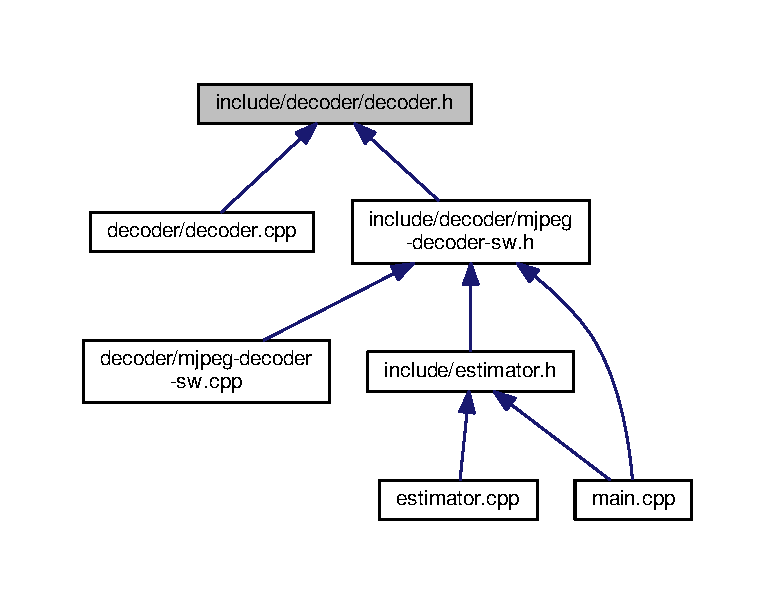
\includegraphics[width=350pt]{decoder_8h__dep__incl}
\end{center}
\end{figure}
\subsection*{Classes}
\begin{DoxyCompactItemize}
\item 
class \hyperlink{classDecoderDevice}{Decoder\+Device}
\end{DoxyCompactItemize}

\hypertarget{mjpeg-decoder-sw_8h}{}\section{include/decoder/mjpeg-\/decoder-\/sw.h File Reference}
\label{mjpeg-decoder-sw_8h}\index{include/decoder/mjpeg-\/decoder-\/sw.\+h@{include/decoder/mjpeg-\/decoder-\/sw.\+h}}
{\ttfamily \#include \char`\"{}decoder/decoder.\+h\char`\"{}}\\*
{\ttfamily \#include $<$stdio.\+h$>$}\\*
{\ttfamily \#include $<$stddef.\+h$>$}\\*
{\ttfamily \#include $<$stdlib.\+h$>$}\\*
{\ttfamily \#include $<$string.\+h$>$}\\*
{\ttfamily \#include $<$jpeglib.\+h$>$}\\*
{\ttfamily \#include $<$setjmp.\+h$>$}\\*
Include dependency graph for mjpeg-\/decoder-\/sw.h\+:
\nopagebreak
\begin{figure}[H]
\begin{center}
\leavevmode
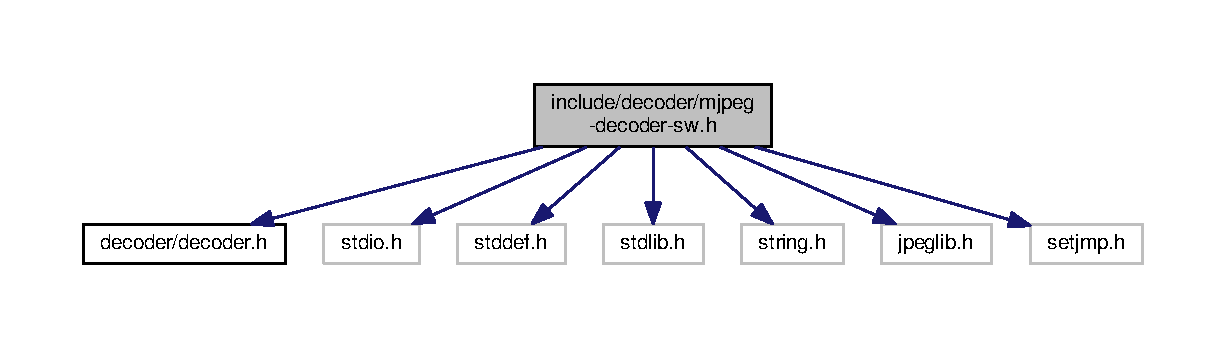
\includegraphics[width=350pt]{mjpeg-decoder-sw_8h__incl}
\end{center}
\end{figure}
This graph shows which files directly or indirectly include this file\+:
\nopagebreak
\begin{figure}[H]
\begin{center}
\leavevmode
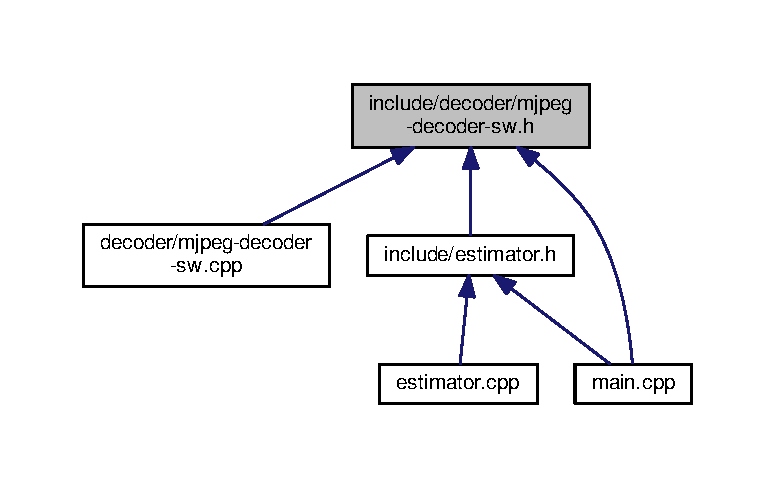
\includegraphics[width=350pt]{mjpeg-decoder-sw_8h__dep__incl}
\end{center}
\end{figure}
\subsection*{Classes}
\begin{DoxyCompactItemize}
\item 
class \hyperlink{classMJPEGDecoderDevice}{M\+J\+P\+E\+G\+Decoder\+Device}
\end{DoxyCompactItemize}

\hypertarget{errors_8h}{}\section{include/errors.h File Reference}
\label{errors_8h}\index{include/errors.\+h@{include/errors.\+h}}
\subsection*{Macros}
\begin{DoxyCompactItemize}
\item 
\#define \hyperlink{errors_8h_add669d31505a077f769cff8e66c780b3}{E\+P\+E\+RM}~1	/$\ast$ Operation not permitted $\ast$/
\item 
\#define \hyperlink{errors_8h_a03e689f378f643d16ea7537918528a48}{E\+N\+O\+E\+NT}~2	/$\ast$ No such file or directory $\ast$/
\item 
\#define \hyperlink{errors_8h_a462e47a8af6288232a5df548221ada4c}{E\+S\+R\+CH}~3	/$\ast$ No such process $\ast$/
\item 
\#define \hyperlink{errors_8h_a46b83d9f6c23b1b65a8cecfd775ddaed}{E\+I\+N\+TR}~4	/$\ast$ Interrupted system call $\ast$/
\item 
\#define \hyperlink{errors_8h_a70979f50f9c83e5aebab3d6a1bd4cf35}{E\+IO}~5	/$\ast$ I/O error $\ast$/
\item 
\#define \hyperlink{errors_8h_a2b3884b11e4932bd372bb6d899d6fbfe}{E\+N\+X\+IO}~6	/$\ast$ No such device or address $\ast$/
\item 
\#define \hyperlink{errors_8h_aba8481985c201ff726f349d7f2d09895}{E2\+B\+IG}~7	/$\ast$ Argument list too long $\ast$/
\item 
\#define \hyperlink{errors_8h_a4d0b1b435ec441e7d50a430b83df5832}{E\+N\+O\+E\+X\+EC}~8	/$\ast$ Exec format error $\ast$/
\item 
\#define \hyperlink{errors_8h_ac54507d66b43ad12f9356257323c0018}{E\+B\+A\+DF}~9	/$\ast$ Bad file number $\ast$/
\item 
\#define \hyperlink{errors_8h_a47b42c351e0e011a048058d224205c0f}{E\+C\+H\+I\+LD}~10	/$\ast$ No child processes $\ast$/
\item 
\#define \hyperlink{errors_8h_af0fac1cea1165b4debec7f686edf3313}{E\+A\+G\+A\+IN}~11	/$\ast$ Try again $\ast$/
\item 
\#define \hyperlink{errors_8h_a6a05c923dad0c1208043e9c20a58c8e5}{E\+N\+O\+M\+EM}~12	/$\ast$ Out of memory $\ast$/
\item 
\#define \hyperlink{errors_8h_ac2a2e9fa555401f94478f74e01868032}{E\+A\+C\+C\+ES}~13	/$\ast$ Permission denied $\ast$/
\item 
\#define \hyperlink{errors_8h_a3f317946e043623f9d6b93dbf60e6316}{E\+F\+A\+U\+LT}~14	/$\ast$ Bad address $\ast$/
\item 
\#define \hyperlink{errors_8h_aa0a4b0e307e83f52be51099f01156936}{E\+N\+O\+T\+B\+LK}~15	/$\ast$ Block device required $\ast$/
\item 
\#define \hyperlink{errors_8h_a8368025077a0385849d6817b2007c095}{E\+B\+U\+SY}~16	/$\ast$ Device or resource busy $\ast$/
\item 
\#define \hyperlink{errors_8h_a0a3bef9e5c47e42917692b5dae3b5498}{E\+E\+X\+I\+ST}~17	/$\ast$ File exists $\ast$/
\item 
\#define \hyperlink{errors_8h_a3396cf9fb0ff5af3a18dd2a2bbdb21e1}{E\+X\+D\+EV}~18	/$\ast$ Cross-\/device link $\ast$/
\item 
\#define \hyperlink{errors_8h_ab9b8cc17d1947160d13faaba7a18d6d1}{E\+N\+O\+D\+EV}~19	/$\ast$ No such device $\ast$/
\item 
\#define \hyperlink{errors_8h_a9262fb92f7ef662d0bdd577912a5b101}{E\+N\+O\+T\+D\+IR}~20	/$\ast$ Not a directory $\ast$/
\item 
\#define \hyperlink{errors_8h_ae22c3a1e0a38f3896de238cc30d0e19b}{E\+I\+S\+D\+IR}~21	/$\ast$ Is a directory $\ast$/
\item 
\#define \hyperlink{errors_8h_a2d1678d5a7cc8ce499643f3b8957def4}{E\+I\+N\+V\+AL}~22	/$\ast$ Invalid argument $\ast$/
\item 
\#define \hyperlink{errors_8h_a5554094b3fb4bb6ebeb0157cb3f82a55}{E\+N\+F\+I\+LE}~23	/$\ast$ File table overflow $\ast$/
\item 
\#define \hyperlink{errors_8h_a64a75c174882ddbfa726c7fd040f87a1}{E\+M\+F\+I\+LE}~24	/$\ast$ Too many open files $\ast$/
\item 
\#define \hyperlink{errors_8h_ac3daf409082bb528032f4452a81e1034}{E\+N\+O\+T\+TY}~25	/$\ast$ Not a typewriter $\ast$/
\item 
\#define \hyperlink{errors_8h_aaed12e82224923d599b6f1939c8e0971}{E\+T\+X\+T\+B\+SY}~26	/$\ast$ Text file busy $\ast$/
\item 
\#define \hyperlink{errors_8h_af5401a500939ed1812c04ca200b95eef}{E\+F\+B\+IG}~27	/$\ast$ File too large $\ast$/
\item 
\#define \hyperlink{errors_8h_a088abe8bad2df798edad3053d719b937}{E\+N\+O\+S\+PC}~28	/$\ast$ No space left on device $\ast$/
\item 
\#define \hyperlink{errors_8h_a0e42d4f9fecdcf5fcca2b333252173c3}{E\+S\+P\+I\+PE}~29	/$\ast$ Illegal seek $\ast$/
\item 
\#define \hyperlink{errors_8h_acb02bb67dddd7ca8cf82634a0781d58d}{E\+R\+O\+FS}~30	/$\ast$ Read-\/only file system $\ast$/
\item 
\#define \hyperlink{errors_8h_a97f59fa1a5a2f61b792c1b9dfc218072}{E\+M\+L\+I\+NK}~31	/$\ast$ Too many links $\ast$/
\item 
\#define \hyperlink{errors_8h_a5f8d33deb08fa27c04897b278ac7f965}{E\+P\+I\+PE}~32	/$\ast$ Broken pipe $\ast$/
\item 
\#define \hyperlink{errors_8h_a5fe247e079b591a68e0fdbf7caec5b70}{E\+D\+OM}~33	/$\ast$ Math argument out of domain of func $\ast$/
\item 
\#define \hyperlink{errors_8h_aa1591a4f3a86360108de5b9ba34980ca}{E\+R\+A\+N\+GE}~34	/$\ast$ Math result not representable $\ast$/
\item 
\#define \hyperlink{errors_8h_aee2672c2fb195944aae9523f563bdc83}{E\+I\+N\+V\+A\+L\+ID}~35
\end{DoxyCompactItemize}


\subsection{Macro Definition Documentation}
\index{errors.\+h@{errors.\+h}!E2\+B\+IG@{E2\+B\+IG}}
\index{E2\+B\+IG@{E2\+B\+IG}!errors.\+h@{errors.\+h}}
\subsubsection[{\texorpdfstring{E2\+B\+IG}{E2BIG}}]{\setlength{\rightskip}{0pt plus 5cm}\#define E2\+B\+IG~7	/$\ast$ Argument list too long $\ast$/}\hypertarget{errors_8h_aba8481985c201ff726f349d7f2d09895}{}\label{errors_8h_aba8481985c201ff726f349d7f2d09895}
\index{errors.\+h@{errors.\+h}!E\+A\+C\+C\+ES@{E\+A\+C\+C\+ES}}
\index{E\+A\+C\+C\+ES@{E\+A\+C\+C\+ES}!errors.\+h@{errors.\+h}}
\subsubsection[{\texorpdfstring{E\+A\+C\+C\+ES}{EACCES}}]{\setlength{\rightskip}{0pt plus 5cm}\#define E\+A\+C\+C\+ES~13	/$\ast$ Permission denied $\ast$/}\hypertarget{errors_8h_ac2a2e9fa555401f94478f74e01868032}{}\label{errors_8h_ac2a2e9fa555401f94478f74e01868032}
\index{errors.\+h@{errors.\+h}!E\+A\+G\+A\+IN@{E\+A\+G\+A\+IN}}
\index{E\+A\+G\+A\+IN@{E\+A\+G\+A\+IN}!errors.\+h@{errors.\+h}}
\subsubsection[{\texorpdfstring{E\+A\+G\+A\+IN}{EAGAIN}}]{\setlength{\rightskip}{0pt plus 5cm}\#define E\+A\+G\+A\+IN~11	/$\ast$ Try again $\ast$/}\hypertarget{errors_8h_af0fac1cea1165b4debec7f686edf3313}{}\label{errors_8h_af0fac1cea1165b4debec7f686edf3313}
\index{errors.\+h@{errors.\+h}!E\+B\+A\+DF@{E\+B\+A\+DF}}
\index{E\+B\+A\+DF@{E\+B\+A\+DF}!errors.\+h@{errors.\+h}}
\subsubsection[{\texorpdfstring{E\+B\+A\+DF}{EBADF}}]{\setlength{\rightskip}{0pt plus 5cm}\#define E\+B\+A\+DF~9	/$\ast$ Bad file number $\ast$/}\hypertarget{errors_8h_ac54507d66b43ad12f9356257323c0018}{}\label{errors_8h_ac54507d66b43ad12f9356257323c0018}
\index{errors.\+h@{errors.\+h}!E\+B\+U\+SY@{E\+B\+U\+SY}}
\index{E\+B\+U\+SY@{E\+B\+U\+SY}!errors.\+h@{errors.\+h}}
\subsubsection[{\texorpdfstring{E\+B\+U\+SY}{EBUSY}}]{\setlength{\rightskip}{0pt plus 5cm}\#define E\+B\+U\+SY~16	/$\ast$ Device or resource busy $\ast$/}\hypertarget{errors_8h_a8368025077a0385849d6817b2007c095}{}\label{errors_8h_a8368025077a0385849d6817b2007c095}
\index{errors.\+h@{errors.\+h}!E\+C\+H\+I\+LD@{E\+C\+H\+I\+LD}}
\index{E\+C\+H\+I\+LD@{E\+C\+H\+I\+LD}!errors.\+h@{errors.\+h}}
\subsubsection[{\texorpdfstring{E\+C\+H\+I\+LD}{ECHILD}}]{\setlength{\rightskip}{0pt plus 5cm}\#define E\+C\+H\+I\+LD~10	/$\ast$ No child processes $\ast$/}\hypertarget{errors_8h_a47b42c351e0e011a048058d224205c0f}{}\label{errors_8h_a47b42c351e0e011a048058d224205c0f}
\index{errors.\+h@{errors.\+h}!E\+D\+OM@{E\+D\+OM}}
\index{E\+D\+OM@{E\+D\+OM}!errors.\+h@{errors.\+h}}
\subsubsection[{\texorpdfstring{E\+D\+OM}{EDOM}}]{\setlength{\rightskip}{0pt plus 5cm}\#define E\+D\+OM~33	/$\ast$ Math argument out of domain of func $\ast$/}\hypertarget{errors_8h_a5fe247e079b591a68e0fdbf7caec5b70}{}\label{errors_8h_a5fe247e079b591a68e0fdbf7caec5b70}
\index{errors.\+h@{errors.\+h}!E\+E\+X\+I\+ST@{E\+E\+X\+I\+ST}}
\index{E\+E\+X\+I\+ST@{E\+E\+X\+I\+ST}!errors.\+h@{errors.\+h}}
\subsubsection[{\texorpdfstring{E\+E\+X\+I\+ST}{EEXIST}}]{\setlength{\rightskip}{0pt plus 5cm}\#define E\+E\+X\+I\+ST~17	/$\ast$ File exists $\ast$/}\hypertarget{errors_8h_a0a3bef9e5c47e42917692b5dae3b5498}{}\label{errors_8h_a0a3bef9e5c47e42917692b5dae3b5498}
\index{errors.\+h@{errors.\+h}!E\+F\+A\+U\+LT@{E\+F\+A\+U\+LT}}
\index{E\+F\+A\+U\+LT@{E\+F\+A\+U\+LT}!errors.\+h@{errors.\+h}}
\subsubsection[{\texorpdfstring{E\+F\+A\+U\+LT}{EFAULT}}]{\setlength{\rightskip}{0pt plus 5cm}\#define E\+F\+A\+U\+LT~14	/$\ast$ Bad address $\ast$/}\hypertarget{errors_8h_a3f317946e043623f9d6b93dbf60e6316}{}\label{errors_8h_a3f317946e043623f9d6b93dbf60e6316}
\index{errors.\+h@{errors.\+h}!E\+F\+B\+IG@{E\+F\+B\+IG}}
\index{E\+F\+B\+IG@{E\+F\+B\+IG}!errors.\+h@{errors.\+h}}
\subsubsection[{\texorpdfstring{E\+F\+B\+IG}{EFBIG}}]{\setlength{\rightskip}{0pt plus 5cm}\#define E\+F\+B\+IG~27	/$\ast$ File too large $\ast$/}\hypertarget{errors_8h_af5401a500939ed1812c04ca200b95eef}{}\label{errors_8h_af5401a500939ed1812c04ca200b95eef}
\index{errors.\+h@{errors.\+h}!E\+I\+N\+TR@{E\+I\+N\+TR}}
\index{E\+I\+N\+TR@{E\+I\+N\+TR}!errors.\+h@{errors.\+h}}
\subsubsection[{\texorpdfstring{E\+I\+N\+TR}{EINTR}}]{\setlength{\rightskip}{0pt plus 5cm}\#define E\+I\+N\+TR~4	/$\ast$ Interrupted system call $\ast$/}\hypertarget{errors_8h_a46b83d9f6c23b1b65a8cecfd775ddaed}{}\label{errors_8h_a46b83d9f6c23b1b65a8cecfd775ddaed}
\index{errors.\+h@{errors.\+h}!E\+I\+N\+V\+AL@{E\+I\+N\+V\+AL}}
\index{E\+I\+N\+V\+AL@{E\+I\+N\+V\+AL}!errors.\+h@{errors.\+h}}
\subsubsection[{\texorpdfstring{E\+I\+N\+V\+AL}{EINVAL}}]{\setlength{\rightskip}{0pt plus 5cm}\#define E\+I\+N\+V\+AL~22	/$\ast$ Invalid argument $\ast$/}\hypertarget{errors_8h_a2d1678d5a7cc8ce499643f3b8957def4}{}\label{errors_8h_a2d1678d5a7cc8ce499643f3b8957def4}
\index{errors.\+h@{errors.\+h}!E\+I\+N\+V\+A\+L\+ID@{E\+I\+N\+V\+A\+L\+ID}}
\index{E\+I\+N\+V\+A\+L\+ID@{E\+I\+N\+V\+A\+L\+ID}!errors.\+h@{errors.\+h}}
\subsubsection[{\texorpdfstring{E\+I\+N\+V\+A\+L\+ID}{EINVALID}}]{\setlength{\rightskip}{0pt plus 5cm}\#define E\+I\+N\+V\+A\+L\+ID~35}\hypertarget{errors_8h_aee2672c2fb195944aae9523f563bdc83}{}\label{errors_8h_aee2672c2fb195944aae9523f563bdc83}
\index{errors.\+h@{errors.\+h}!E\+IO@{E\+IO}}
\index{E\+IO@{E\+IO}!errors.\+h@{errors.\+h}}
\subsubsection[{\texorpdfstring{E\+IO}{EIO}}]{\setlength{\rightskip}{0pt plus 5cm}\#define E\+IO~5	/$\ast$ I/O error $\ast$/}\hypertarget{errors_8h_a70979f50f9c83e5aebab3d6a1bd4cf35}{}\label{errors_8h_a70979f50f9c83e5aebab3d6a1bd4cf35}
\index{errors.\+h@{errors.\+h}!E\+I\+S\+D\+IR@{E\+I\+S\+D\+IR}}
\index{E\+I\+S\+D\+IR@{E\+I\+S\+D\+IR}!errors.\+h@{errors.\+h}}
\subsubsection[{\texorpdfstring{E\+I\+S\+D\+IR}{EISDIR}}]{\setlength{\rightskip}{0pt plus 5cm}\#define E\+I\+S\+D\+IR~21	/$\ast$ Is a directory $\ast$/}\hypertarget{errors_8h_ae22c3a1e0a38f3896de238cc30d0e19b}{}\label{errors_8h_ae22c3a1e0a38f3896de238cc30d0e19b}
\index{errors.\+h@{errors.\+h}!E\+M\+F\+I\+LE@{E\+M\+F\+I\+LE}}
\index{E\+M\+F\+I\+LE@{E\+M\+F\+I\+LE}!errors.\+h@{errors.\+h}}
\subsubsection[{\texorpdfstring{E\+M\+F\+I\+LE}{EMFILE}}]{\setlength{\rightskip}{0pt plus 5cm}\#define E\+M\+F\+I\+LE~24	/$\ast$ Too many open files $\ast$/}\hypertarget{errors_8h_a64a75c174882ddbfa726c7fd040f87a1}{}\label{errors_8h_a64a75c174882ddbfa726c7fd040f87a1}
\index{errors.\+h@{errors.\+h}!E\+M\+L\+I\+NK@{E\+M\+L\+I\+NK}}
\index{E\+M\+L\+I\+NK@{E\+M\+L\+I\+NK}!errors.\+h@{errors.\+h}}
\subsubsection[{\texorpdfstring{E\+M\+L\+I\+NK}{EMLINK}}]{\setlength{\rightskip}{0pt plus 5cm}\#define E\+M\+L\+I\+NK~31	/$\ast$ Too many links $\ast$/}\hypertarget{errors_8h_a97f59fa1a5a2f61b792c1b9dfc218072}{}\label{errors_8h_a97f59fa1a5a2f61b792c1b9dfc218072}
\index{errors.\+h@{errors.\+h}!E\+N\+F\+I\+LE@{E\+N\+F\+I\+LE}}
\index{E\+N\+F\+I\+LE@{E\+N\+F\+I\+LE}!errors.\+h@{errors.\+h}}
\subsubsection[{\texorpdfstring{E\+N\+F\+I\+LE}{ENFILE}}]{\setlength{\rightskip}{0pt plus 5cm}\#define E\+N\+F\+I\+LE~23	/$\ast$ File table overflow $\ast$/}\hypertarget{errors_8h_a5554094b3fb4bb6ebeb0157cb3f82a55}{}\label{errors_8h_a5554094b3fb4bb6ebeb0157cb3f82a55}
\index{errors.\+h@{errors.\+h}!E\+N\+O\+D\+EV@{E\+N\+O\+D\+EV}}
\index{E\+N\+O\+D\+EV@{E\+N\+O\+D\+EV}!errors.\+h@{errors.\+h}}
\subsubsection[{\texorpdfstring{E\+N\+O\+D\+EV}{ENODEV}}]{\setlength{\rightskip}{0pt plus 5cm}\#define E\+N\+O\+D\+EV~19	/$\ast$ No such device $\ast$/}\hypertarget{errors_8h_ab9b8cc17d1947160d13faaba7a18d6d1}{}\label{errors_8h_ab9b8cc17d1947160d13faaba7a18d6d1}
\index{errors.\+h@{errors.\+h}!E\+N\+O\+E\+NT@{E\+N\+O\+E\+NT}}
\index{E\+N\+O\+E\+NT@{E\+N\+O\+E\+NT}!errors.\+h@{errors.\+h}}
\subsubsection[{\texorpdfstring{E\+N\+O\+E\+NT}{ENOENT}}]{\setlength{\rightskip}{0pt plus 5cm}\#define E\+N\+O\+E\+NT~2	/$\ast$ No such file or directory $\ast$/}\hypertarget{errors_8h_a03e689f378f643d16ea7537918528a48}{}\label{errors_8h_a03e689f378f643d16ea7537918528a48}
\index{errors.\+h@{errors.\+h}!E\+N\+O\+E\+X\+EC@{E\+N\+O\+E\+X\+EC}}
\index{E\+N\+O\+E\+X\+EC@{E\+N\+O\+E\+X\+EC}!errors.\+h@{errors.\+h}}
\subsubsection[{\texorpdfstring{E\+N\+O\+E\+X\+EC}{ENOEXEC}}]{\setlength{\rightskip}{0pt plus 5cm}\#define E\+N\+O\+E\+X\+EC~8	/$\ast$ Exec format error $\ast$/}\hypertarget{errors_8h_a4d0b1b435ec441e7d50a430b83df5832}{}\label{errors_8h_a4d0b1b435ec441e7d50a430b83df5832}
\index{errors.\+h@{errors.\+h}!E\+N\+O\+M\+EM@{E\+N\+O\+M\+EM}}
\index{E\+N\+O\+M\+EM@{E\+N\+O\+M\+EM}!errors.\+h@{errors.\+h}}
\subsubsection[{\texorpdfstring{E\+N\+O\+M\+EM}{ENOMEM}}]{\setlength{\rightskip}{0pt plus 5cm}\#define E\+N\+O\+M\+EM~12	/$\ast$ Out of memory $\ast$/}\hypertarget{errors_8h_a6a05c923dad0c1208043e9c20a58c8e5}{}\label{errors_8h_a6a05c923dad0c1208043e9c20a58c8e5}
\index{errors.\+h@{errors.\+h}!E\+N\+O\+S\+PC@{E\+N\+O\+S\+PC}}
\index{E\+N\+O\+S\+PC@{E\+N\+O\+S\+PC}!errors.\+h@{errors.\+h}}
\subsubsection[{\texorpdfstring{E\+N\+O\+S\+PC}{ENOSPC}}]{\setlength{\rightskip}{0pt plus 5cm}\#define E\+N\+O\+S\+PC~28	/$\ast$ No space left on device $\ast$/}\hypertarget{errors_8h_a088abe8bad2df798edad3053d719b937}{}\label{errors_8h_a088abe8bad2df798edad3053d719b937}
\index{errors.\+h@{errors.\+h}!E\+N\+O\+T\+B\+LK@{E\+N\+O\+T\+B\+LK}}
\index{E\+N\+O\+T\+B\+LK@{E\+N\+O\+T\+B\+LK}!errors.\+h@{errors.\+h}}
\subsubsection[{\texorpdfstring{E\+N\+O\+T\+B\+LK}{ENOTBLK}}]{\setlength{\rightskip}{0pt plus 5cm}\#define E\+N\+O\+T\+B\+LK~15	/$\ast$ Block device required $\ast$/}\hypertarget{errors_8h_aa0a4b0e307e83f52be51099f01156936}{}\label{errors_8h_aa0a4b0e307e83f52be51099f01156936}
\index{errors.\+h@{errors.\+h}!E\+N\+O\+T\+D\+IR@{E\+N\+O\+T\+D\+IR}}
\index{E\+N\+O\+T\+D\+IR@{E\+N\+O\+T\+D\+IR}!errors.\+h@{errors.\+h}}
\subsubsection[{\texorpdfstring{E\+N\+O\+T\+D\+IR}{ENOTDIR}}]{\setlength{\rightskip}{0pt plus 5cm}\#define E\+N\+O\+T\+D\+IR~20	/$\ast$ Not a directory $\ast$/}\hypertarget{errors_8h_a9262fb92f7ef662d0bdd577912a5b101}{}\label{errors_8h_a9262fb92f7ef662d0bdd577912a5b101}
\index{errors.\+h@{errors.\+h}!E\+N\+O\+T\+TY@{E\+N\+O\+T\+TY}}
\index{E\+N\+O\+T\+TY@{E\+N\+O\+T\+TY}!errors.\+h@{errors.\+h}}
\subsubsection[{\texorpdfstring{E\+N\+O\+T\+TY}{ENOTTY}}]{\setlength{\rightskip}{0pt plus 5cm}\#define E\+N\+O\+T\+TY~25	/$\ast$ Not a typewriter $\ast$/}\hypertarget{errors_8h_ac3daf409082bb528032f4452a81e1034}{}\label{errors_8h_ac3daf409082bb528032f4452a81e1034}
\index{errors.\+h@{errors.\+h}!E\+N\+X\+IO@{E\+N\+X\+IO}}
\index{E\+N\+X\+IO@{E\+N\+X\+IO}!errors.\+h@{errors.\+h}}
\subsubsection[{\texorpdfstring{E\+N\+X\+IO}{ENXIO}}]{\setlength{\rightskip}{0pt plus 5cm}\#define E\+N\+X\+IO~6	/$\ast$ No such device or address $\ast$/}\hypertarget{errors_8h_a2b3884b11e4932bd372bb6d899d6fbfe}{}\label{errors_8h_a2b3884b11e4932bd372bb6d899d6fbfe}
\index{errors.\+h@{errors.\+h}!E\+P\+E\+RM@{E\+P\+E\+RM}}
\index{E\+P\+E\+RM@{E\+P\+E\+RM}!errors.\+h@{errors.\+h}}
\subsubsection[{\texorpdfstring{E\+P\+E\+RM}{EPERM}}]{\setlength{\rightskip}{0pt plus 5cm}\#define E\+P\+E\+RM~1	/$\ast$ Operation not permitted $\ast$/}\hypertarget{errors_8h_add669d31505a077f769cff8e66c780b3}{}\label{errors_8h_add669d31505a077f769cff8e66c780b3}
\index{errors.\+h@{errors.\+h}!E\+P\+I\+PE@{E\+P\+I\+PE}}
\index{E\+P\+I\+PE@{E\+P\+I\+PE}!errors.\+h@{errors.\+h}}
\subsubsection[{\texorpdfstring{E\+P\+I\+PE}{EPIPE}}]{\setlength{\rightskip}{0pt plus 5cm}\#define E\+P\+I\+PE~32	/$\ast$ Broken pipe $\ast$/}\hypertarget{errors_8h_a5f8d33deb08fa27c04897b278ac7f965}{}\label{errors_8h_a5f8d33deb08fa27c04897b278ac7f965}
\index{errors.\+h@{errors.\+h}!E\+R\+A\+N\+GE@{E\+R\+A\+N\+GE}}
\index{E\+R\+A\+N\+GE@{E\+R\+A\+N\+GE}!errors.\+h@{errors.\+h}}
\subsubsection[{\texorpdfstring{E\+R\+A\+N\+GE}{ERANGE}}]{\setlength{\rightskip}{0pt plus 5cm}\#define E\+R\+A\+N\+GE~34	/$\ast$ Math result not representable $\ast$/}\hypertarget{errors_8h_aa1591a4f3a86360108de5b9ba34980ca}{}\label{errors_8h_aa1591a4f3a86360108de5b9ba34980ca}
\index{errors.\+h@{errors.\+h}!E\+R\+O\+FS@{E\+R\+O\+FS}}
\index{E\+R\+O\+FS@{E\+R\+O\+FS}!errors.\+h@{errors.\+h}}
\subsubsection[{\texorpdfstring{E\+R\+O\+FS}{EROFS}}]{\setlength{\rightskip}{0pt plus 5cm}\#define E\+R\+O\+FS~30	/$\ast$ Read-\/only file system $\ast$/}\hypertarget{errors_8h_acb02bb67dddd7ca8cf82634a0781d58d}{}\label{errors_8h_acb02bb67dddd7ca8cf82634a0781d58d}
\index{errors.\+h@{errors.\+h}!E\+S\+P\+I\+PE@{E\+S\+P\+I\+PE}}
\index{E\+S\+P\+I\+PE@{E\+S\+P\+I\+PE}!errors.\+h@{errors.\+h}}
\subsubsection[{\texorpdfstring{E\+S\+P\+I\+PE}{ESPIPE}}]{\setlength{\rightskip}{0pt plus 5cm}\#define E\+S\+P\+I\+PE~29	/$\ast$ Illegal seek $\ast$/}\hypertarget{errors_8h_a0e42d4f9fecdcf5fcca2b333252173c3}{}\label{errors_8h_a0e42d4f9fecdcf5fcca2b333252173c3}
\index{errors.\+h@{errors.\+h}!E\+S\+R\+CH@{E\+S\+R\+CH}}
\index{E\+S\+R\+CH@{E\+S\+R\+CH}!errors.\+h@{errors.\+h}}
\subsubsection[{\texorpdfstring{E\+S\+R\+CH}{ESRCH}}]{\setlength{\rightskip}{0pt plus 5cm}\#define E\+S\+R\+CH~3	/$\ast$ No such process $\ast$/}\hypertarget{errors_8h_a462e47a8af6288232a5df548221ada4c}{}\label{errors_8h_a462e47a8af6288232a5df548221ada4c}
\index{errors.\+h@{errors.\+h}!E\+T\+X\+T\+B\+SY@{E\+T\+X\+T\+B\+SY}}
\index{E\+T\+X\+T\+B\+SY@{E\+T\+X\+T\+B\+SY}!errors.\+h@{errors.\+h}}
\subsubsection[{\texorpdfstring{E\+T\+X\+T\+B\+SY}{ETXTBSY}}]{\setlength{\rightskip}{0pt plus 5cm}\#define E\+T\+X\+T\+B\+SY~26	/$\ast$ Text file busy $\ast$/}\hypertarget{errors_8h_aaed12e82224923d599b6f1939c8e0971}{}\label{errors_8h_aaed12e82224923d599b6f1939c8e0971}
\index{errors.\+h@{errors.\+h}!E\+X\+D\+EV@{E\+X\+D\+EV}}
\index{E\+X\+D\+EV@{E\+X\+D\+EV}!errors.\+h@{errors.\+h}}
\subsubsection[{\texorpdfstring{E\+X\+D\+EV}{EXDEV}}]{\setlength{\rightskip}{0pt plus 5cm}\#define E\+X\+D\+EV~18	/$\ast$ Cross-\/device link $\ast$/}\hypertarget{errors_8h_a3396cf9fb0ff5af3a18dd2a2bbdb21e1}{}\label{errors_8h_a3396cf9fb0ff5af3a18dd2a2bbdb21e1}

\hypertarget{estimator_8h}{}\section{include/estimator.h File Reference}
\label{estimator_8h}\index{include/estimator.\+h@{include/estimator.\+h}}
{\ttfamily \#include \char`\"{}opencv2/opencv.\+hpp\char`\"{}}\\*
{\ttfamily \#include \char`\"{}opencv2/calib3d/calib3d.\+hpp\char`\"{}}\\*
{\ttfamily \#include \char`\"{}opencv2/imgproc.\+hpp\char`\"{}}\\*
{\ttfamily \#include \char`\"{}opencv2/imgcodecs.\+hpp\char`\"{}}\\*
{\ttfamily \#include \char`\"{}opencv2/highgui.\+hpp\char`\"{}}\\*
{\ttfamily \#include \char`\"{}opencv2/core/utility.\+hpp\char`\"{}}\\*
{\ttfamily \#include $<$iostream$>$}\\*
{\ttfamily \#include $<$string.\+h$>$}\\*
{\ttfamily \#include \char`\"{}math.\+h\char`\"{}}\\*
{\ttfamily \#include $<$iomanip$>$}\\*
{\ttfamily \#include \char`\"{}debug.\+h\char`\"{}}\\*
{\ttfamily \#include $<$signal.\+h$>$}\\*
{\ttfamily \#include $<$unistd.\+h$>$}\\*
{\ttfamily \#include \char`\"{}decoder/mjpeg-\/decoder-\/sw.\+h\char`\"{}}\\*
{\ttfamily \#include \char`\"{}stream/v4l2-\/stream-\/stereo-\/device.\+h\char`\"{}}\\*
{\ttfamily \#include \char`\"{}opencv2/ximgproc/disparity\+\_\+filter.\+hpp\char`\"{}}\\*
{\ttfamily \#include \char`\"{}helper.\+h\char`\"{}}\\*
{\ttfamily \#include \char`\"{}filter/filter.\+h\char`\"{}}\\*
{\ttfamily \#include \char`\"{}stereo-\/matcher/stereo-\/matcher.\+h\char`\"{}}\\*
{\ttfamily \#include \char`\"{}utils/cmdline-\/parser.\+h\char`\"{}}\\*
Include dependency graph for estimator.\+h\+:
\nopagebreak
\begin{figure}[H]
\begin{center}
\leavevmode
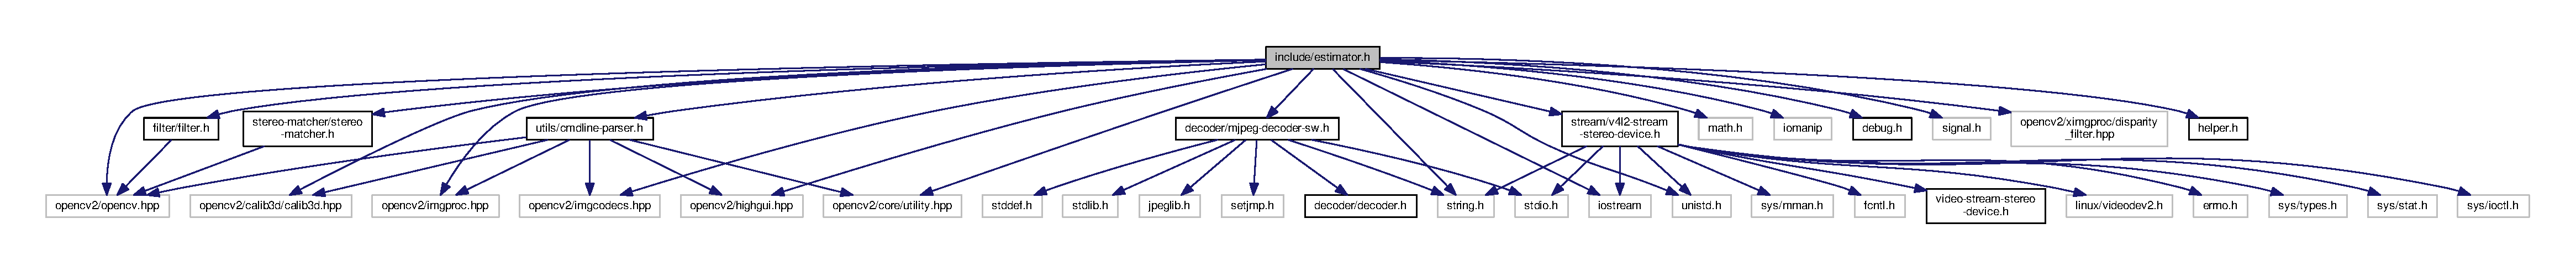
\includegraphics[width=350pt]{estimator_8h__incl}
\end{center}
\end{figure}
This graph shows which files directly or indirectly include this file\+:
\nopagebreak
\begin{figure}[H]
\begin{center}
\leavevmode
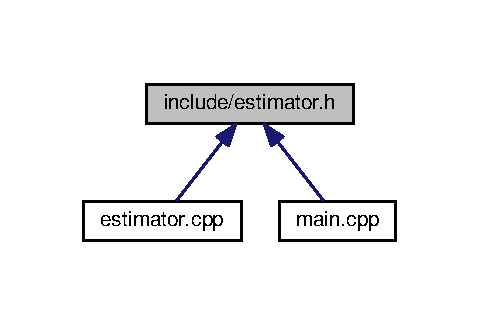
\includegraphics[width=230pt]{estimator_8h__dep__incl}
\end{center}
\end{figure}
\subsection*{Classes}
\begin{DoxyCompactItemize}
\item 
struct \hyperlink{structexec__time__struct}{exec\+\_\+time\+\_\+struct}
\item 
class \hyperlink{classEstimator}{Estimator}
\end{DoxyCompactItemize}
\subsection*{Macros}
\begin{DoxyCompactItemize}
\item 
\#define \hyperlink{estimator_8h_a27c8cca253b95065a21f4eafcc6bf026}{M\+E\+A\+S\+U\+R\+E\+\_\+\+E\+X\+E\+C\+U\+T\+I\+O\+N\+\_\+\+T\+I\+M\+E\+\_\+\+S\+T\+A\+RT}
\item 
\#define \hyperlink{estimator_8h_a6b508f4c70a2ddfefabb7e0075a032a9}{M\+E\+A\+S\+U\+R\+E\+\_\+\+E\+X\+E\+C\+U\+T\+I\+O\+N\+\_\+\+T\+I\+ME}(\+\_\+fn\+\_\+)~\+\_\+fn\+\_\+;
\item 
\#define \hyperlink{estimator_8h_acc2dee67ff0b6fd8f68f7f74f718b46c}{M\+E\+A\+S\+U\+R\+E\+\_\+\+E\+X\+E\+C\+U\+T\+I\+O\+N\+\_\+\+T\+I\+M\+E\+\_\+\+E\+ND}
\end{DoxyCompactItemize}


\subsection{Macro Definition Documentation}
\index{estimator.\+h@{estimator.\+h}!M\+E\+A\+S\+U\+R\+E\+\_\+\+E\+X\+E\+C\+U\+T\+I\+O\+N\+\_\+\+T\+I\+ME@{M\+E\+A\+S\+U\+R\+E\+\_\+\+E\+X\+E\+C\+U\+T\+I\+O\+N\+\_\+\+T\+I\+ME}}
\index{M\+E\+A\+S\+U\+R\+E\+\_\+\+E\+X\+E\+C\+U\+T\+I\+O\+N\+\_\+\+T\+I\+ME@{M\+E\+A\+S\+U\+R\+E\+\_\+\+E\+X\+E\+C\+U\+T\+I\+O\+N\+\_\+\+T\+I\+ME}!estimator.\+h@{estimator.\+h}}
\subsubsection[{\texorpdfstring{M\+E\+A\+S\+U\+R\+E\+\_\+\+E\+X\+E\+C\+U\+T\+I\+O\+N\+\_\+\+T\+I\+ME}{MEASURE_EXECUTION_TIME}}]{\setlength{\rightskip}{0pt plus 5cm}\#define M\+E\+A\+S\+U\+R\+E\+\_\+\+E\+X\+E\+C\+U\+T\+I\+O\+N\+\_\+\+T\+I\+ME(
\begin{DoxyParamCaption}
\item[{}]{\+\_\+fn\+\_\+}
\end{DoxyParamCaption}
)~\+\_\+fn\+\_\+;}\hypertarget{estimator_8h_a6b508f4c70a2ddfefabb7e0075a032a9}{}\label{estimator_8h_a6b508f4c70a2ddfefabb7e0075a032a9}
\index{estimator.\+h@{estimator.\+h}!M\+E\+A\+S\+U\+R\+E\+\_\+\+E\+X\+E\+C\+U\+T\+I\+O\+N\+\_\+\+T\+I\+M\+E\+\_\+\+E\+ND@{M\+E\+A\+S\+U\+R\+E\+\_\+\+E\+X\+E\+C\+U\+T\+I\+O\+N\+\_\+\+T\+I\+M\+E\+\_\+\+E\+ND}}
\index{M\+E\+A\+S\+U\+R\+E\+\_\+\+E\+X\+E\+C\+U\+T\+I\+O\+N\+\_\+\+T\+I\+M\+E\+\_\+\+E\+ND@{M\+E\+A\+S\+U\+R\+E\+\_\+\+E\+X\+E\+C\+U\+T\+I\+O\+N\+\_\+\+T\+I\+M\+E\+\_\+\+E\+ND}!estimator.\+h@{estimator.\+h}}
\subsubsection[{\texorpdfstring{M\+E\+A\+S\+U\+R\+E\+\_\+\+E\+X\+E\+C\+U\+T\+I\+O\+N\+\_\+\+T\+I\+M\+E\+\_\+\+E\+ND}{MEASURE_EXECUTION_TIME_END}}]{\setlength{\rightskip}{0pt plus 5cm}\#define M\+E\+A\+S\+U\+R\+E\+\_\+\+E\+X\+E\+C\+U\+T\+I\+O\+N\+\_\+\+T\+I\+M\+E\+\_\+\+E\+ND}\hypertarget{estimator_8h_acc2dee67ff0b6fd8f68f7f74f718b46c}{}\label{estimator_8h_acc2dee67ff0b6fd8f68f7f74f718b46c}
\index{estimator.\+h@{estimator.\+h}!M\+E\+A\+S\+U\+R\+E\+\_\+\+E\+X\+E\+C\+U\+T\+I\+O\+N\+\_\+\+T\+I\+M\+E\+\_\+\+S\+T\+A\+RT@{M\+E\+A\+S\+U\+R\+E\+\_\+\+E\+X\+E\+C\+U\+T\+I\+O\+N\+\_\+\+T\+I\+M\+E\+\_\+\+S\+T\+A\+RT}}
\index{M\+E\+A\+S\+U\+R\+E\+\_\+\+E\+X\+E\+C\+U\+T\+I\+O\+N\+\_\+\+T\+I\+M\+E\+\_\+\+S\+T\+A\+RT@{M\+E\+A\+S\+U\+R\+E\+\_\+\+E\+X\+E\+C\+U\+T\+I\+O\+N\+\_\+\+T\+I\+M\+E\+\_\+\+S\+T\+A\+RT}!estimator.\+h@{estimator.\+h}}
\subsubsection[{\texorpdfstring{M\+E\+A\+S\+U\+R\+E\+\_\+\+E\+X\+E\+C\+U\+T\+I\+O\+N\+\_\+\+T\+I\+M\+E\+\_\+\+S\+T\+A\+RT}{MEASURE_EXECUTION_TIME_START}}]{\setlength{\rightskip}{0pt plus 5cm}\#define M\+E\+A\+S\+U\+R\+E\+\_\+\+E\+X\+E\+C\+U\+T\+I\+O\+N\+\_\+\+T\+I\+M\+E\+\_\+\+S\+T\+A\+RT}\hypertarget{estimator_8h_a27c8cca253b95065a21f4eafcc6bf026}{}\label{estimator_8h_a27c8cca253b95065a21f4eafcc6bf026}

\hypertarget{filter_8h}{}\section{include/filter/filter.h File Reference}
\label{filter_8h}\index{include/filter/filter.\+h@{include/filter/filter.\+h}}
{\ttfamily \#include \char`\"{}opencv2/opencv.\+hpp\char`\"{}}\\*
Include dependency graph for filter.\+h\+:
\nopagebreak
\begin{figure}[H]
\begin{center}
\leavevmode
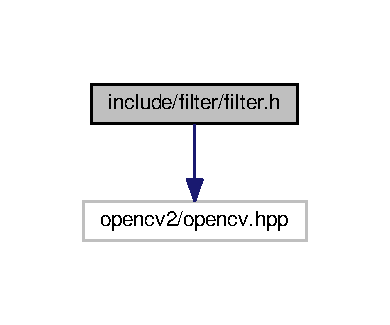
\includegraphics[width=187pt]{filter_8h__incl}
\end{center}
\end{figure}
This graph shows which files directly or indirectly include this file\+:
\nopagebreak
\begin{figure}[H]
\begin{center}
\leavevmode
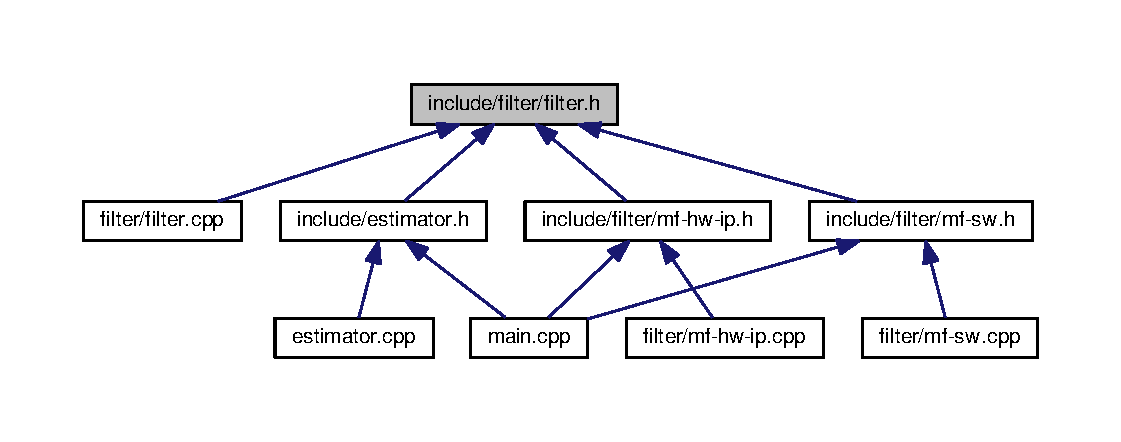
\includegraphics[width=350pt]{filter_8h__dep__incl}
\end{center}
\end{figure}
\subsection*{Classes}
\begin{DoxyCompactItemize}
\item 
class \hyperlink{classVideoFilterDevice}{Video\+Filter\+Device}
\end{DoxyCompactItemize}

\hypertarget{mf-hw-ip_8h}{}\section{include/filter/mf-\/hw-\/ip.h File Reference}
\label{mf-hw-ip_8h}\index{include/filter/mf-\/hw-\/ip.\+h@{include/filter/mf-\/hw-\/ip.\+h}}
{\ttfamily \#include \char`\"{}filter/filter.\+h\char`\"{}}\\*
{\ttfamily \#include $<$stdint.\+h$>$}\\*
{\ttfamily \#include $<$assert.\+h$>$}\\*
{\ttfamily \#include $<$dirent.\+h$>$}\\*
{\ttfamily \#include $<$fcntl.\+h$>$}\\*
{\ttfamily \#include $<$stdio.\+h$>$}\\*
{\ttfamily \#include $<$stdlib.\+h$>$}\\*
{\ttfamily \#include $<$string.\+h$>$}\\*
{\ttfamily \#include $<$sys/mman.\+h$>$}\\*
{\ttfamily \#include $<$unistd.\+h$>$}\\*
{\ttfamily \#include $<$stddef.\+h$>$}\\*
{\ttfamily \#include $<$sys/stat.\+h$>$}\\*
{\ttfamily \#include $<$math.\+h$>$}\\*
{\ttfamily \#include $<$sys/types.\+h$>$}\\*
{\ttfamily \#include $<$sys/ioctl.\+h$>$}\\*
{\ttfamily \#include \char`\"{}opencv2/opencv.\+hpp\char`\"{}}\\*
{\ttfamily \#include \char`\"{}uio.\+h\char`\"{}}\\*
{\ttfamily \#include \char`\"{}io.\+h\char`\"{}}\\*
Include dependency graph for mf-\/hw-\/ip.h\+:
\nopagebreak
\begin{figure}[H]
\begin{center}
\leavevmode
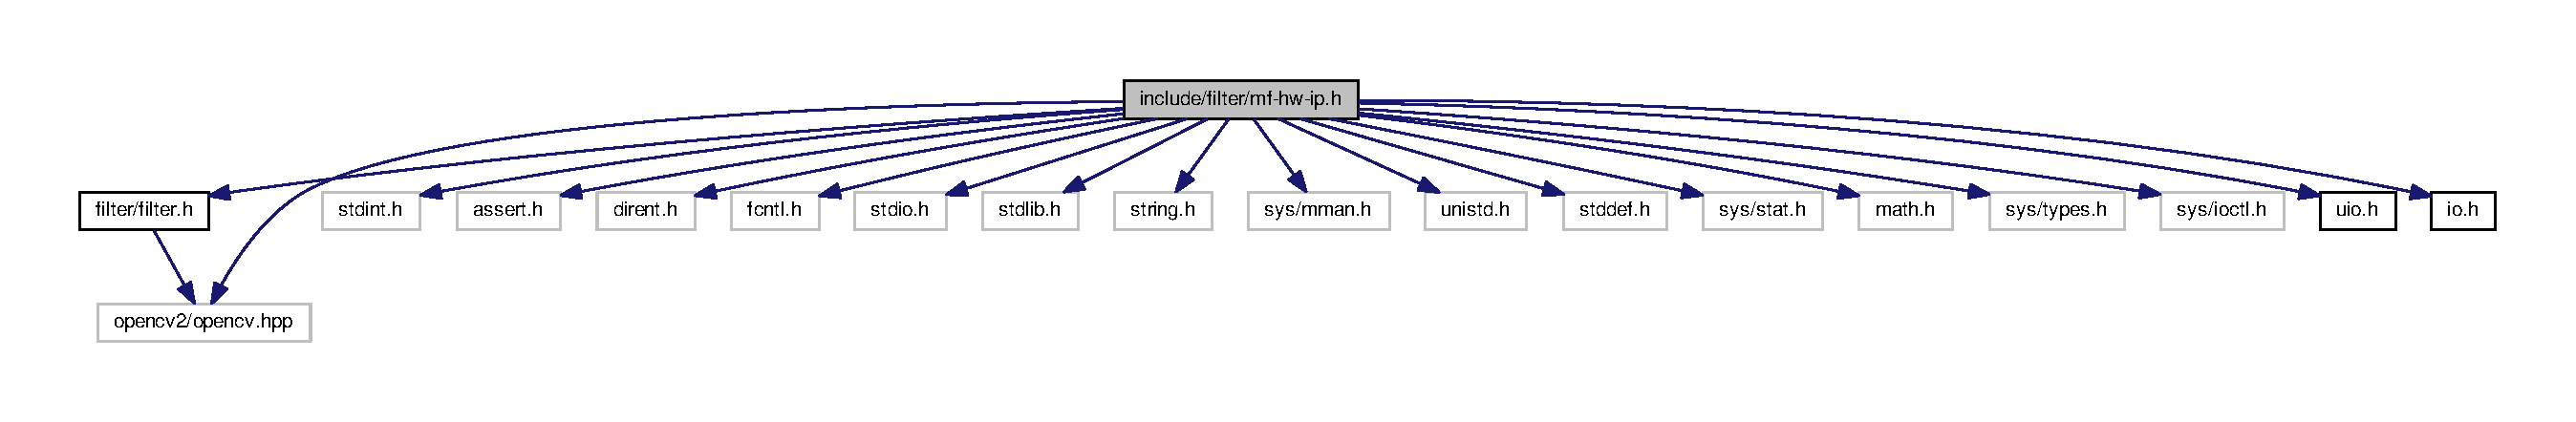
\includegraphics[width=350pt]{mf-hw-ip_8h__incl}
\end{center}
\end{figure}
This graph shows which files directly or indirectly include this file\+:
\nopagebreak
\begin{figure}[H]
\begin{center}
\leavevmode
\includegraphics[width=250pt]{mf-hw-ip_8h__dep__incl}
\end{center}
\end{figure}
\subsection*{Classes}
\begin{DoxyCompactItemize}
\item 
struct \hyperlink{structvdma__transfer__dim}{vdma\+\_\+transfer\+\_\+dim}
\item 
struct \hyperlink{structxmorph__filter__uio__map}{xmorph\+\_\+filter\+\_\+uio\+\_\+map}
\item 
struct \hyperlink{structxmorph__filter__uio__info}{xmorph\+\_\+filter\+\_\+uio\+\_\+info}
\item 
class \hyperlink{classHWMorphologicalFilterIPCore}{H\+W\+Morphological\+Filter\+I\+P\+Core}
\end{DoxyCompactItemize}

\hypertarget{mf-sw_8h}{}\section{include/filter/mf-\/sw.h File Reference}
\label{mf-sw_8h}\index{include/filter/mf-\/sw.\+h@{include/filter/mf-\/sw.\+h}}
{\ttfamily \#include \char`\"{}filter/filter.\+h\char`\"{}}\\*
{\ttfamily \#include \char`\"{}opencv2/opencv.\+hpp\char`\"{}}\\*
Include dependency graph for mf-\/sw.h\+:
\nopagebreak
\begin{figure}[H]
\begin{center}
\leavevmode
\includegraphics[width=196pt]{mf-sw_8h__incl}
\end{center}
\end{figure}
This graph shows which files directly or indirectly include this file\+:
\nopagebreak
\begin{figure}[H]
\begin{center}
\leavevmode
\includegraphics[width=238pt]{mf-sw_8h__dep__incl}
\end{center}
\end{figure}
\subsection*{Classes}
\begin{DoxyCompactItemize}
\item 
class \hyperlink{classSWMorphologicalFilter}{S\+W\+Morphological\+Filter}
\end{DoxyCompactItemize}
\subsection*{Macros}
\begin{DoxyCompactItemize}
\item 
\#define \hyperlink{mf-sw_8h_a306e2bb4acdc55bf9dd3c719ad1e425c}{M\+O\+R\+P\+H\+\_\+\+F\+I\+L\+T\+E\+R\+\_\+\+DX}~10
\item 
\#define \hyperlink{mf-sw_8h_a0a459c81c9d83cc1aba0b3a87ec9177f}{M\+O\+R\+P\+H\+\_\+\+F\+I\+L\+T\+E\+R\+\_\+\+DY}~10
\end{DoxyCompactItemize}


\subsection{Macro Definition Documentation}
\index{mf-\/sw.\+h@{mf-\/sw.\+h}!M\+O\+R\+P\+H\+\_\+\+F\+I\+L\+T\+E\+R\+\_\+\+DX@{M\+O\+R\+P\+H\+\_\+\+F\+I\+L\+T\+E\+R\+\_\+\+DX}}
\index{M\+O\+R\+P\+H\+\_\+\+F\+I\+L\+T\+E\+R\+\_\+\+DX@{M\+O\+R\+P\+H\+\_\+\+F\+I\+L\+T\+E\+R\+\_\+\+DX}!mf-\/sw.\+h@{mf-\/sw.\+h}}
\subsubsection[{\texorpdfstring{M\+O\+R\+P\+H\+\_\+\+F\+I\+L\+T\+E\+R\+\_\+\+DX}{MORPH_FILTER_DX}}]{\setlength{\rightskip}{0pt plus 5cm}\#define M\+O\+R\+P\+H\+\_\+\+F\+I\+L\+T\+E\+R\+\_\+\+DX~10}\hypertarget{mf-sw_8h_a306e2bb4acdc55bf9dd3c719ad1e425c}{}\label{mf-sw_8h_a306e2bb4acdc55bf9dd3c719ad1e425c}
\index{mf-\/sw.\+h@{mf-\/sw.\+h}!M\+O\+R\+P\+H\+\_\+\+F\+I\+L\+T\+E\+R\+\_\+\+DY@{M\+O\+R\+P\+H\+\_\+\+F\+I\+L\+T\+E\+R\+\_\+\+DY}}
\index{M\+O\+R\+P\+H\+\_\+\+F\+I\+L\+T\+E\+R\+\_\+\+DY@{M\+O\+R\+P\+H\+\_\+\+F\+I\+L\+T\+E\+R\+\_\+\+DY}!mf-\/sw.\+h@{mf-\/sw.\+h}}
\subsubsection[{\texorpdfstring{M\+O\+R\+P\+H\+\_\+\+F\+I\+L\+T\+E\+R\+\_\+\+DY}{MORPH_FILTER_DY}}]{\setlength{\rightskip}{0pt plus 5cm}\#define M\+O\+R\+P\+H\+\_\+\+F\+I\+L\+T\+E\+R\+\_\+\+DY~10}\hypertarget{mf-sw_8h_a0a459c81c9d83cc1aba0b3a87ec9177f}{}\label{mf-sw_8h_a0a459c81c9d83cc1aba0b3a87ec9177f}

\hypertarget{helper_8h}{}\section{include/helper.h File Reference}
\label{helper_8h}\index{include/helper.\+h@{include/helper.\+h}}
This graph shows which files directly or indirectly include this file\+:
\nopagebreak
\begin{figure}[H]
\begin{center}
\leavevmode
\includegraphics[width=236pt]{helper_8h__dep__incl}
\end{center}
\end{figure}
\subsection*{Macros}
\begin{DoxyCompactItemize}
\item 
\#define \hyperlink{helper_8h_a0d77409489a4b407e12c9b2b600e2621}{A\+R\+R\+A\+Y\+\_\+\+S\+I\+ZE}(\+\_\+\+A\+\_\+)~sizeof(\+\_\+\+A\+\_\+)/sizeof(\+\_\+\+A\+\_\+\mbox{[}0\mbox{]})
\end{DoxyCompactItemize}


\subsection{Macro Definition Documentation}
\index{helper.\+h@{helper.\+h}!A\+R\+R\+A\+Y\+\_\+\+S\+I\+ZE@{A\+R\+R\+A\+Y\+\_\+\+S\+I\+ZE}}
\index{A\+R\+R\+A\+Y\+\_\+\+S\+I\+ZE@{A\+R\+R\+A\+Y\+\_\+\+S\+I\+ZE}!helper.\+h@{helper.\+h}}
\subsubsection[{\texorpdfstring{A\+R\+R\+A\+Y\+\_\+\+S\+I\+ZE}{ARRAY_SIZE}}]{\setlength{\rightskip}{0pt plus 5cm}\#define A\+R\+R\+A\+Y\+\_\+\+S\+I\+ZE(
\begin{DoxyParamCaption}
\item[{}]{\+\_\+\+A\+\_\+}
\end{DoxyParamCaption}
)~sizeof(\+\_\+\+A\+\_\+)/sizeof(\+\_\+\+A\+\_\+\mbox{[}0\mbox{]})}\hypertarget{helper_8h_a0d77409489a4b407e12c9b2b600e2621}{}\label{helper_8h_a0d77409489a4b407e12c9b2b600e2621}

\hypertarget{io_8h}{}\section{include/io.h File Reference}
\label{io_8h}\index{include/io.\+h@{include/io.\+h}}
This graph shows which files directly or indirectly include this file\+:
\nopagebreak
\begin{figure}[H]
\begin{center}
\leavevmode
\includegraphics[width=350pt]{io_8h__dep__incl}
\end{center}
\end{figure}
\subsection*{Macros}
\begin{DoxyCompactItemize}
\item 
\#define \hyperlink{io_8h_ad78b8ecd62091db07f830edc048c25ca}{\+\_\+\+\_\+io\+\_\+mem}~volatile
\item 
\#define \hyperlink{io_8h_a2ee2e87a6f91c5b29fabb7fe0b958a6f}{\+\_\+\+\_\+io}~volatile
\end{DoxyCompactItemize}


\subsection{Macro Definition Documentation}
\index{io.\+h@{io.\+h}!\+\_\+\+\_\+io@{\+\_\+\+\_\+io}}
\index{\+\_\+\+\_\+io@{\+\_\+\+\_\+io}!io.\+h@{io.\+h}}
\subsubsection[{\texorpdfstring{\+\_\+\+\_\+io}{__io}}]{\setlength{\rightskip}{0pt plus 5cm}\#define \+\_\+\+\_\+io~volatile}\hypertarget{io_8h_a2ee2e87a6f91c5b29fabb7fe0b958a6f}{}\label{io_8h_a2ee2e87a6f91c5b29fabb7fe0b958a6f}
\index{io.\+h@{io.\+h}!\+\_\+\+\_\+io\+\_\+mem@{\+\_\+\+\_\+io\+\_\+mem}}
\index{\+\_\+\+\_\+io\+\_\+mem@{\+\_\+\+\_\+io\+\_\+mem}!io.\+h@{io.\+h}}
\subsubsection[{\texorpdfstring{\+\_\+\+\_\+io\+\_\+mem}{__io_mem}}]{\setlength{\rightskip}{0pt plus 5cm}\#define \+\_\+\+\_\+io\+\_\+mem~volatile}\hypertarget{io_8h_ad78b8ecd62091db07f830edc048c25ca}{}\label{io_8h_ad78b8ecd62091db07f830edc048c25ca}

\hypertarget{bm-hw-ip_8h}{}\section{include/stereo-\/matcher/bm-\/hw-\/ip.h File Reference}
\label{bm-hw-ip_8h}\index{include/stereo-\/matcher/bm-\/hw-\/ip.\+h@{include/stereo-\/matcher/bm-\/hw-\/ip.\+h}}
{\ttfamily \#include \char`\"{}stereo-\/matcher/stereo-\/matcher.\+h\char`\"{}}\\*
{\ttfamily \#include \char`\"{}opencv2/calib3d/calib3d.\+hpp\char`\"{}}\\*
{\ttfamily \#include \char`\"{}opencv2/imgproc.\+hpp\char`\"{}}\\*
{\ttfamily \#include \char`\"{}opencv2/imgcodecs.\+hpp\char`\"{}}\\*
{\ttfamily \#include \char`\"{}opencv2/highgui.\+hpp\char`\"{}}\\*
{\ttfamily \#include \char`\"{}opencv2/core/utility.\+hpp\char`\"{}}\\*
{\ttfamily \#include \char`\"{}opencv2/ximgproc/disparity\+\_\+filter.\+hpp\char`\"{}}\\*
{\ttfamily \#include $<$iostream$>$}\\*
{\ttfamily \#include $<$string.\+h$>$}\\*
{\ttfamily \#include \char`\"{}math.\+h\char`\"{}}\\*
{\ttfamily \#include \char`\"{}debug.\+h\char`\"{}}\\*
{\ttfamily \#include $<$stdint.\+h$>$}\\*
{\ttfamily \#include $<$assert.\+h$>$}\\*
{\ttfamily \#include $<$dirent.\+h$>$}\\*
{\ttfamily \#include $<$fcntl.\+h$>$}\\*
{\ttfamily \#include $<$stdio.\+h$>$}\\*
{\ttfamily \#include $<$stdlib.\+h$>$}\\*
{\ttfamily \#include $<$sys/mman.\+h$>$}\\*
{\ttfamily \#include $<$unistd.\+h$>$}\\*
{\ttfamily \#include $<$stddef.\+h$>$}\\*
{\ttfamily \#include $<$sys/stat.\+h$>$}\\*
{\ttfamily \#include $<$cstdint$>$}\\*
{\ttfamily \#include \char`\"{}uio.\+h\char`\"{}}\\*
Include dependency graph for bm-\/hw-\/ip.h\+:
\nopagebreak
\begin{figure}[H]
\begin{center}
\leavevmode
\includegraphics[width=350pt]{bm-hw-ip_8h__incl}
\end{center}
\end{figure}
This graph shows which files directly or indirectly include this file\+:
\nopagebreak
\begin{figure}[H]
\begin{center}
\leavevmode
\includegraphics[width=268pt]{bm-hw-ip_8h__dep__incl}
\end{center}
\end{figure}
\subsection*{Classes}
\begin{DoxyCompactItemize}
\item 
struct \hyperlink{structdcx__config}{dcx\+\_\+config}
\item 
struct \hyperlink{structdcx__device}{dcx\+\_\+device}
\item 
struct \hyperlink{structdcx__uio__map}{dcx\+\_\+uio\+\_\+map}
\item 
struct \hyperlink{structdcx__uio__info}{dcx\+\_\+uio\+\_\+info}
\item 
class \hyperlink{classHWMatcherDisparityCoprocessor}{H\+W\+Matcher\+Disparity\+Coprocessor}
\end{DoxyCompactItemize}

\hypertarget{bm-sw_8h}{}\section{include/stereo-\/matcher/bm-\/sw.h File Reference}
\label{bm-sw_8h}\index{include/stereo-\/matcher/bm-\/sw.\+h@{include/stereo-\/matcher/bm-\/sw.\+h}}
{\ttfamily \#include \char`\"{}stereo-\/matcher/stereo-\/matcher.\+h\char`\"{}}\\*
{\ttfamily \#include \char`\"{}opencv2/calib3d/calib3d.\+hpp\char`\"{}}\\*
{\ttfamily \#include \char`\"{}opencv2/imgproc.\+hpp\char`\"{}}\\*
{\ttfamily \#include \char`\"{}opencv2/imgcodecs.\+hpp\char`\"{}}\\*
{\ttfamily \#include \char`\"{}opencv2/highgui.\+hpp\char`\"{}}\\*
{\ttfamily \#include \char`\"{}opencv2/core/utility.\+hpp\char`\"{}}\\*
{\ttfamily \#include \char`\"{}opencv2/ximgproc/disparity\+\_\+filter.\+hpp\char`\"{}}\\*
{\ttfamily \#include $<$iostream$>$}\\*
{\ttfamily \#include $<$string.\+h$>$}\\*
{\ttfamily \#include \char`\"{}math.\+h\char`\"{}}\\*
{\ttfamily \#include \char`\"{}debug.\+h\char`\"{}}\\*
Include dependency graph for bm-\/sw.h\+:
\nopagebreak
\begin{figure}[H]
\begin{center}
\leavevmode
\includegraphics[width=350pt]{bm-sw_8h__incl}
\end{center}
\end{figure}
This graph shows which files directly or indirectly include this file\+:
\nopagebreak
\begin{figure}[H]
\begin{center}
\leavevmode
\includegraphics[width=288pt]{bm-sw_8h__dep__incl}
\end{center}
\end{figure}
\subsection*{Classes}
\begin{DoxyCompactItemize}
\item 
class \hyperlink{classSWMatcherKonolige}{S\+W\+Matcher\+Konolige}
\end{DoxyCompactItemize}

\hypertarget{sgbm-sw_8h}{}\section{include/stereo-\/matcher/sgbm-\/sw.h File Reference}
\label{sgbm-sw_8h}\index{include/stereo-\/matcher/sgbm-\/sw.\+h@{include/stereo-\/matcher/sgbm-\/sw.\+h}}
{\ttfamily \#include \char`\"{}stereo-\/matcher/stereo-\/matcher.\+h\char`\"{}}\\*
{\ttfamily \#include \char`\"{}opencv2/calib3d/calib3d.\+hpp\char`\"{}}\\*
{\ttfamily \#include \char`\"{}opencv2/imgproc.\+hpp\char`\"{}}\\*
{\ttfamily \#include \char`\"{}opencv2/imgcodecs.\+hpp\char`\"{}}\\*
{\ttfamily \#include \char`\"{}opencv2/highgui.\+hpp\char`\"{}}\\*
{\ttfamily \#include \char`\"{}opencv2/core/utility.\+hpp\char`\"{}}\\*
{\ttfamily \#include \char`\"{}opencv2/ximgproc/disparity\+\_\+filter.\+hpp\char`\"{}}\\*
{\ttfamily \#include $<$iostream$>$}\\*
{\ttfamily \#include $<$string.\+h$>$}\\*
{\ttfamily \#include \char`\"{}math.\+h\char`\"{}}\\*
{\ttfamily \#include \char`\"{}debug.\+h\char`\"{}}\\*
Include dependency graph for sgbm-\/sw.h\+:
\nopagebreak
\begin{figure}[H]
\begin{center}
\leavevmode
\includegraphics[width=350pt]{sgbm-sw_8h__incl}
\end{center}
\end{figure}
This graph shows which files directly or indirectly include this file\+:
\nopagebreak
\begin{figure}[H]
\begin{center}
\leavevmode
\includegraphics[width=264pt]{sgbm-sw_8h__dep__incl}
\end{center}
\end{figure}
\subsection*{Classes}
\begin{DoxyCompactItemize}
\item 
class \hyperlink{classSWSemiGlobalMatcher}{S\+W\+Semi\+Global\+Matcher}
\end{DoxyCompactItemize}

\hypertarget{stereo-matcher_8h}{}\section{include/stereo-\/matcher/stereo-\/matcher.h File Reference}
\label{stereo-matcher_8h}\index{include/stereo-\/matcher/stereo-\/matcher.\+h@{include/stereo-\/matcher/stereo-\/matcher.\+h}}
{\ttfamily \#include \char`\"{}opencv2/opencv.\+hpp\char`\"{}}\\*
Include dependency graph for stereo-\/matcher.h\+:
\nopagebreak
\begin{figure}[H]
\begin{center}
\leavevmode
\includegraphics[width=196pt]{stereo-matcher_8h__incl}
\end{center}
\end{figure}
This graph shows which files directly or indirectly include this file\+:
\nopagebreak
\begin{figure}[H]
\begin{center}
\leavevmode
\includegraphics[width=350pt]{stereo-matcher_8h__dep__incl}
\end{center}
\end{figure}
\subsection*{Classes}
\begin{DoxyCompactItemize}
\item 
class \hyperlink{classBlockMatcher}{Block\+Matcher}
\end{DoxyCompactItemize}

\hypertarget{v4l2-stream-stereo-device_8h}{}\section{include/stream/v4l2-\/stream-\/stereo-\/device.h File Reference}
\label{v4l2-stream-stereo-device_8h}\index{include/stream/v4l2-\/stream-\/stereo-\/device.\+h@{include/stream/v4l2-\/stream-\/stereo-\/device.\+h}}
{\ttfamily \#include $<$linux/videodev2.\+h$>$}\\*
{\ttfamily \#include $<$iostream$>$}\\*
{\ttfamily \#include $<$stdio.\+h$>$}\\*
{\ttfamily \#include $<$errno.\+h$>$}\\*
{\ttfamily \#include $<$unistd.\+h$>$}\\*
{\ttfamily \#include $<$sys/types.\+h$>$}\\*
{\ttfamily \#include $<$sys/stat.\+h$>$}\\*
{\ttfamily \#include $<$sys/ioctl.\+h$>$}\\*
{\ttfamily \#include $<$sys/mman.\+h$>$}\\*
{\ttfamily \#include $<$fcntl.\+h$>$}\\*
{\ttfamily \#include $<$string.\+h$>$}\\*
{\ttfamily \#include \char`\"{}video-\/stream-\/stereo-\/device.\+h\char`\"{}}\\*
Include dependency graph for v4l2-\/stream-\/stereo-\/device.h\+:
\nopagebreak
\begin{figure}[H]
\begin{center}
\leavevmode
\includegraphics[width=350pt]{v4l2-stream-stereo-device_8h__incl}
\end{center}
\end{figure}
This graph shows which files directly or indirectly include this file\+:
\nopagebreak
\begin{figure}[H]
\begin{center}
\leavevmode
\includegraphics[width=337pt]{v4l2-stream-stereo-device_8h__dep__incl}
\end{center}
\end{figure}
\subsection*{Classes}
\begin{DoxyCompactItemize}
\item 
class \hyperlink{classV4LStreamStereoDevice}{V4\+L\+Stream\+Stereo\+Device}
\end{DoxyCompactItemize}

\hypertarget{video-stream-stereo-device_8h}{}\section{include/stream/video-\/stream-\/stereo-\/device.h File Reference}
\label{video-stream-stereo-device_8h}\index{include/stream/video-\/stream-\/stereo-\/device.\+h@{include/stream/video-\/stream-\/stereo-\/device.\+h}}
This graph shows which files directly or indirectly include this file\+:
\nopagebreak
\begin{figure}[H]
\begin{center}
\leavevmode
\includegraphics[width=350pt]{video-stream-stereo-device_8h__dep__incl}
\end{center}
\end{figure}
\subsection*{Classes}
\begin{DoxyCompactItemize}
\item 
struct \hyperlink{structvideoStreamBuffer}{video\+Stream\+Buffer}
\item 
class \hyperlink{classVideoStreamStereoDevice}{Video\+Stream\+Stereo\+Device}
\end{DoxyCompactItemize}

\hypertarget{uio_8h}{}\section{include/uio.h File Reference}
\label{uio_8h}\index{include/uio.\+h@{include/uio.\+h}}
This graph shows which files directly or indirectly include this file\+:
\nopagebreak
\begin{figure}[H]
\begin{center}
\leavevmode
\includegraphics[width=350pt]{uio_8h__dep__incl}
\end{center}
\end{figure}
\subsection*{Macros}
\begin{DoxyCompactItemize}
\item 
\#define \hyperlink{uio_8h_abef5d45a73f9956460621ec93bb04259}{M\+A\+X\+\_\+\+U\+I\+O\+\_\+\+P\+A\+T\+H\+\_\+\+S\+I\+ZE}~256
\item 
\#define \hyperlink{uio_8h_a5ed3f1c67d5551770a91ef53fe208c83}{M\+A\+X\+\_\+\+U\+I\+O\+\_\+\+N\+A\+M\+E\+\_\+\+S\+I\+ZE}~64
\item 
\#define \hyperlink{uio_8h_a05a77cb47b9d8cdaaee64df37627ffdc}{M\+A\+X\+\_\+\+U\+I\+O\+\_\+\+M\+A\+PS}~5
\item 
\#define \hyperlink{uio_8h_a3946fb1f8faf4d351dc0ebef828b65e5}{U\+I\+O\+\_\+\+I\+N\+V\+A\+L\+I\+D\+\_\+\+A\+D\+DR}~0
\end{DoxyCompactItemize}


\subsection{Macro Definition Documentation}
\index{uio.\+h@{uio.\+h}!M\+A\+X\+\_\+\+U\+I\+O\+\_\+\+M\+A\+PS@{M\+A\+X\+\_\+\+U\+I\+O\+\_\+\+M\+A\+PS}}
\index{M\+A\+X\+\_\+\+U\+I\+O\+\_\+\+M\+A\+PS@{M\+A\+X\+\_\+\+U\+I\+O\+\_\+\+M\+A\+PS}!uio.\+h@{uio.\+h}}
\subsubsection[{\texorpdfstring{M\+A\+X\+\_\+\+U\+I\+O\+\_\+\+M\+A\+PS}{MAX_UIO_MAPS}}]{\setlength{\rightskip}{0pt plus 5cm}\#define M\+A\+X\+\_\+\+U\+I\+O\+\_\+\+M\+A\+PS~5}\hypertarget{uio_8h_a05a77cb47b9d8cdaaee64df37627ffdc}{}\label{uio_8h_a05a77cb47b9d8cdaaee64df37627ffdc}
\index{uio.\+h@{uio.\+h}!M\+A\+X\+\_\+\+U\+I\+O\+\_\+\+N\+A\+M\+E\+\_\+\+S\+I\+ZE@{M\+A\+X\+\_\+\+U\+I\+O\+\_\+\+N\+A\+M\+E\+\_\+\+S\+I\+ZE}}
\index{M\+A\+X\+\_\+\+U\+I\+O\+\_\+\+N\+A\+M\+E\+\_\+\+S\+I\+ZE@{M\+A\+X\+\_\+\+U\+I\+O\+\_\+\+N\+A\+M\+E\+\_\+\+S\+I\+ZE}!uio.\+h@{uio.\+h}}
\subsubsection[{\texorpdfstring{M\+A\+X\+\_\+\+U\+I\+O\+\_\+\+N\+A\+M\+E\+\_\+\+S\+I\+ZE}{MAX_UIO_NAME_SIZE}}]{\setlength{\rightskip}{0pt plus 5cm}\#define M\+A\+X\+\_\+\+U\+I\+O\+\_\+\+N\+A\+M\+E\+\_\+\+S\+I\+ZE~64}\hypertarget{uio_8h_a5ed3f1c67d5551770a91ef53fe208c83}{}\label{uio_8h_a5ed3f1c67d5551770a91ef53fe208c83}
\index{uio.\+h@{uio.\+h}!M\+A\+X\+\_\+\+U\+I\+O\+\_\+\+P\+A\+T\+H\+\_\+\+S\+I\+ZE@{M\+A\+X\+\_\+\+U\+I\+O\+\_\+\+P\+A\+T\+H\+\_\+\+S\+I\+ZE}}
\index{M\+A\+X\+\_\+\+U\+I\+O\+\_\+\+P\+A\+T\+H\+\_\+\+S\+I\+ZE@{M\+A\+X\+\_\+\+U\+I\+O\+\_\+\+P\+A\+T\+H\+\_\+\+S\+I\+ZE}!uio.\+h@{uio.\+h}}
\subsubsection[{\texorpdfstring{M\+A\+X\+\_\+\+U\+I\+O\+\_\+\+P\+A\+T\+H\+\_\+\+S\+I\+ZE}{MAX_UIO_PATH_SIZE}}]{\setlength{\rightskip}{0pt plus 5cm}\#define M\+A\+X\+\_\+\+U\+I\+O\+\_\+\+P\+A\+T\+H\+\_\+\+S\+I\+ZE~256}\hypertarget{uio_8h_abef5d45a73f9956460621ec93bb04259}{}\label{uio_8h_abef5d45a73f9956460621ec93bb04259}
\index{uio.\+h@{uio.\+h}!U\+I\+O\+\_\+\+I\+N\+V\+A\+L\+I\+D\+\_\+\+A\+D\+DR@{U\+I\+O\+\_\+\+I\+N\+V\+A\+L\+I\+D\+\_\+\+A\+D\+DR}}
\index{U\+I\+O\+\_\+\+I\+N\+V\+A\+L\+I\+D\+\_\+\+A\+D\+DR@{U\+I\+O\+\_\+\+I\+N\+V\+A\+L\+I\+D\+\_\+\+A\+D\+DR}!uio.\+h@{uio.\+h}}
\subsubsection[{\texorpdfstring{U\+I\+O\+\_\+\+I\+N\+V\+A\+L\+I\+D\+\_\+\+A\+D\+DR}{UIO_INVALID_ADDR}}]{\setlength{\rightskip}{0pt plus 5cm}\#define U\+I\+O\+\_\+\+I\+N\+V\+A\+L\+I\+D\+\_\+\+A\+D\+DR~0}\hypertarget{uio_8h_a3946fb1f8faf4d351dc0ebef828b65e5}{}\label{uio_8h_a3946fb1f8faf4d351dc0ebef828b65e5}

\hypertarget{cmdline-parser_8h}{}\section{include/utils/cmdline-\/parser.h File Reference}
\label{cmdline-parser_8h}\index{include/utils/cmdline-\/parser.\+h@{include/utils/cmdline-\/parser.\+h}}
{\ttfamily \#include \char`\"{}opencv2/opencv.\+hpp\char`\"{}}\\*
{\ttfamily \#include \char`\"{}opencv2/calib3d/calib3d.\+hpp\char`\"{}}\\*
{\ttfamily \#include \char`\"{}opencv2/imgproc.\+hpp\char`\"{}}\\*
{\ttfamily \#include \char`\"{}opencv2/imgcodecs.\+hpp\char`\"{}}\\*
{\ttfamily \#include \char`\"{}opencv2/highgui.\+hpp\char`\"{}}\\*
{\ttfamily \#include \char`\"{}opencv2/core/utility.\+hpp\char`\"{}}\\*
Include dependency graph for cmdline-\/parser.h\+:
\nopagebreak
\begin{figure}[H]
\begin{center}
\leavevmode
\includegraphics[width=350pt]{cmdline-parser_8h__incl}
\end{center}
\end{figure}
This graph shows which files directly or indirectly include this file\+:
\nopagebreak
\begin{figure}[H]
\begin{center}
\leavevmode
\includegraphics[width=350pt]{cmdline-parser_8h__dep__incl}
\end{center}
\end{figure}
\subsection*{Classes}
\begin{DoxyCompactItemize}
\item 
class \hyperlink{classEstimatorCmdLineParser}{Estimator\+Cmd\+Line\+Parser}
\end{DoxyCompactItemize}

\hypertarget{main_8cpp}{}\section{main.\+cpp File Reference}
\label{main_8cpp}\index{main.\+cpp@{main.\+cpp}}
{\ttfamily \#include \char`\"{}opencv2/opencv.\+hpp\char`\"{}}\\*
{\ttfamily \#include \char`\"{}opencv2/calib3d/calib3d.\+hpp\char`\"{}}\\*
{\ttfamily \#include \char`\"{}opencv2/imgproc.\+hpp\char`\"{}}\\*
{\ttfamily \#include \char`\"{}opencv2/imgcodecs.\+hpp\char`\"{}}\\*
{\ttfamily \#include \char`\"{}opencv2/highgui.\+hpp\char`\"{}}\\*
{\ttfamily \#include \char`\"{}opencv2/core/utility.\+hpp\char`\"{}}\\*
{\ttfamily \#include $<$iostream$>$}\\*
{\ttfamily \#include $<$string.\+h$>$}\\*
{\ttfamily \#include \char`\"{}math.\+h\char`\"{}}\\*
{\ttfamily \#include $<$iomanip$>$}\\*
{\ttfamily \#include \char`\"{}debug.\+h\char`\"{}}\\*
{\ttfamily \#include $<$signal.\+h$>$}\\*
{\ttfamily \#include $<$unistd.\+h$>$}\\*
{\ttfamily \#include \char`\"{}decoder/mjpeg-\/decoder-\/sw.\+h\char`\"{}}\\*
{\ttfamily \#include \char`\"{}stream/v4l2-\/stream-\/stereo-\/device.\+h\char`\"{}}\\*
{\ttfamily \#include \char`\"{}include/filter/mf-\/sw.\+h\char`\"{}}\\*
{\ttfamily \#include \char`\"{}stereo-\/matcher/bm-\/sw.\+h\char`\"{}}\\*
{\ttfamily \#include \char`\"{}stereo-\/matcher/sgbm-\/sw.\+h\char`\"{}}\\*
{\ttfamily \#include \char`\"{}stereo-\/matcher/bm-\/hw-\/ip.\+h\char`\"{}}\\*
{\ttfamily \#include \char`\"{}filter/mf-\/hw-\/ip.\+h\char`\"{}}\\*
{\ttfamily \#include \char`\"{}utils/cmdline-\/parser.\+h\char`\"{}}\\*
{\ttfamily \#include \char`\"{}helper.\+h\char`\"{}}\\*
{\ttfamily \#include \char`\"{}estimator.\+h\char`\"{}}\\*
Include dependency graph for main.\+cpp\+:
\nopagebreak
\begin{figure}[H]
\begin{center}
\leavevmode
\includegraphics[width=350pt]{main_8cpp__incl}
\end{center}
\end{figure}
\subsection*{Classes}
\begin{DoxyCompactItemize}
\item 
struct \hyperlink{structhsv__object__ranges}{hsv\+\_\+object\+\_\+ranges}
\end{DoxyCompactItemize}
\subsection*{Functions}
\begin{DoxyCompactItemize}
\item 
int \hyperlink{main_8cpp_a3c04138a5bfe5d72780bb7e82a18e627}{main} (int argc, char $\ast$$\ast$argv)
\end{DoxyCompactItemize}


\subsection{Function Documentation}
\index{main.\+cpp@{main.\+cpp}!main@{main}}
\index{main@{main}!main.\+cpp@{main.\+cpp}}
\subsubsection[{\texorpdfstring{main(int argc, char $\ast$$\ast$argv)}{main(int argc, char **argv)}}]{\setlength{\rightskip}{0pt plus 5cm}int main (
\begin{DoxyParamCaption}
\item[{int}]{argc, }
\item[{char $\ast$$\ast$}]{argv}
\end{DoxyParamCaption}
)}\hypertarget{main_8cpp_a3c04138a5bfe5d72780bb7e82a18e627}{}\label{main_8cpp_a3c04138a5bfe5d72780bb7e82a18e627}

\hypertarget{README_8md}{}\section{R\+E\+A\+D\+M\+E.\+md File Reference}
\label{README_8md}\index{R\+E\+A\+D\+M\+E.\+md@{R\+E\+A\+D\+M\+E.\+md}}

\hypertarget{bm-hw-ip_8cpp}{}\section{stereo-\/matcher/bm-\/hw-\/ip.cpp File Reference}
\label{bm-hw-ip_8cpp}\index{stereo-\/matcher/bm-\/hw-\/ip.\+cpp@{stereo-\/matcher/bm-\/hw-\/ip.\+cpp}}
{\ttfamily \#include \char`\"{}stereo-\/matcher/bm-\/hw-\/ip.\+h\char`\"{}}\\*
{\ttfamily \#include $<$stdlib.\+h$>$}\\*
{\ttfamily \#include \char`\"{}debug.\+h\char`\"{}}\\*
{\ttfamily \#include \char`\"{}string.\+h\char`\"{}}\\*
{\ttfamily \#include \char`\"{}io.\+h\char`\"{}}\\*
Include dependency graph for bm-\/hw-\/ip.cpp\+:
\nopagebreak
\begin{figure}[H]
\begin{center}
\leavevmode
\includegraphics[width=350pt]{bm-hw-ip_8cpp__incl}
\end{center}
\end{figure}
\subsection*{Macros}
\begin{DoxyCompactItemize}
\item 
\#define \hyperlink{bm-hw-ip_8cpp_a54d979456c9969a8cf5132ee39a4c9bc}{M\+A\+X\+\_\+\+D\+I\+SP}~12
\item 
\#define \hyperlink{bm-hw-ip_8cpp_a435f899ff44eecd8e0dedd26c624a151}{C\+T\+R\+L\+\_\+\+B\+PP}~0x10
\item 
\#define \hyperlink{bm-hw-ip_8cpp_aeb96a2577ceac361cd96b403eca35044}{C\+T\+R\+L\+\_\+\+X\+D\+IM}~0x18
\item 
\#define \hyperlink{bm-hw-ip_8cpp_aaa61d5823190114e006260fb733e5e82}{C\+T\+R\+L\+\_\+\+Y\+D\+IM}~0x20
\item 
\#define \hyperlink{bm-hw-ip_8cpp_a3c2719c36b69d32310520966b8027d28}{C\+T\+R\+L\+\_\+\+C\+U\+R\+R\+E\+N\+T\+\_\+\+R\+OW}~0x28
\item 
\#define \hyperlink{bm-hw-ip_8cpp_a13f23608dca3cf0b939c586f2aef961f}{C\+T\+R\+L\+\_\+\+C\+U\+R\+R\+E\+N\+T\+\_\+\+R\+O\+W\+\_\+\+C\+T\+RL}~0x2c
\item 
\#define \hyperlink{bm-hw-ip_8cpp_ae9c1de4d1f380d0d1acf46b0cf88456e}{C\+T\+R\+L\+\_\+\+M\+A\+X\+D\+I\+S\+P\+A\+R\+I\+TY}~0x30
\item 
\#define \hyperlink{bm-hw-ip_8cpp_a18f79d86a6a5a36f2e9f72630af88923}{A\+X\+I\+L\+I\+T\+E\+S\+\_\+\+A\+P\+\_\+\+C\+T\+RL}~0x00
\item 
\#define \hyperlink{bm-hw-ip_8cpp_a202988bcd3de3dcacdc550382b76bb10}{A\+X\+I\+L\+I\+T\+E\+S\+\_\+\+G\+IE}~0x04
\item 
\#define \hyperlink{bm-hw-ip_8cpp_af118e9c8e023df34cfd732022ffc5052}{A\+X\+I\+L\+I\+T\+E\+S\+\_\+\+I\+ER}~0x08
\item 
\#define \hyperlink{bm-hw-ip_8cpp_acf88b636ca246d88ca4dc8bb4d803ce1}{A\+X\+I\+L\+I\+T\+E\+S\+\_\+\+I\+SR}~0x0c
\item 
\#define \hyperlink{bm-hw-ip_8cpp_a2c2fe3f7d9f197adf0be653cd7f5afda}{A\+X\+I\+L\+I\+T\+E\+S\+\_\+\+A\+P\+\_\+\+R\+E\+T\+U\+RN}~0x10
\item 
\#define \hyperlink{bm-hw-ip_8cpp_a8f1d02722e7ff7d91defc351a1575e52}{A\+X\+I\+L\+I\+T\+E\+S\+\_\+\+L\+E\+FT}~0x18
\item 
\#define \hyperlink{bm-hw-ip_8cpp_a2859628312a9a269821eda5c9e1a5db4}{A\+X\+I\+L\+I\+T\+E\+S\+\_\+\+R\+I\+G\+HT}~0x20
\item 
\#define \hyperlink{bm-hw-ip_8cpp_a26b21b4be758a8e27ef77a4fa51d0640}{A\+X\+I\+L\+I\+T\+E\+S\+\_\+\+O\+U\+T\+P\+UT}~0x28
\item 
\#define \hyperlink{bm-hw-ip_8cpp_a6f4ae195d2c5d14f499036d7b7952fed}{A\+P\+\_\+\+E\+N\+\_\+\+B\+IT}~0U
\item 
\#define \hyperlink{bm-hw-ip_8cpp_ac41f006533297629f93c22fa60bf910d}{A\+P\+\_\+\+D\+O\+N\+E\+\_\+\+B\+IT}~1U
\end{DoxyCompactItemize}


\subsection{Macro Definition Documentation}
\index{bm-\/hw-\/ip.\+cpp@{bm-\/hw-\/ip.\+cpp}!A\+P\+\_\+\+D\+O\+N\+E\+\_\+\+B\+IT@{A\+P\+\_\+\+D\+O\+N\+E\+\_\+\+B\+IT}}
\index{A\+P\+\_\+\+D\+O\+N\+E\+\_\+\+B\+IT@{A\+P\+\_\+\+D\+O\+N\+E\+\_\+\+B\+IT}!bm-\/hw-\/ip.\+cpp@{bm-\/hw-\/ip.\+cpp}}
\subsubsection[{\texorpdfstring{A\+P\+\_\+\+D\+O\+N\+E\+\_\+\+B\+IT}{AP_DONE_BIT}}]{\setlength{\rightskip}{0pt plus 5cm}\#define A\+P\+\_\+\+D\+O\+N\+E\+\_\+\+B\+IT~1U}\hypertarget{bm-hw-ip_8cpp_ac41f006533297629f93c22fa60bf910d}{}\label{bm-hw-ip_8cpp_ac41f006533297629f93c22fa60bf910d}
\index{bm-\/hw-\/ip.\+cpp@{bm-\/hw-\/ip.\+cpp}!A\+P\+\_\+\+E\+N\+\_\+\+B\+IT@{A\+P\+\_\+\+E\+N\+\_\+\+B\+IT}}
\index{A\+P\+\_\+\+E\+N\+\_\+\+B\+IT@{A\+P\+\_\+\+E\+N\+\_\+\+B\+IT}!bm-\/hw-\/ip.\+cpp@{bm-\/hw-\/ip.\+cpp}}
\subsubsection[{\texorpdfstring{A\+P\+\_\+\+E\+N\+\_\+\+B\+IT}{AP_EN_BIT}}]{\setlength{\rightskip}{0pt plus 5cm}\#define A\+P\+\_\+\+E\+N\+\_\+\+B\+IT~0U}\hypertarget{bm-hw-ip_8cpp_a6f4ae195d2c5d14f499036d7b7952fed}{}\label{bm-hw-ip_8cpp_a6f4ae195d2c5d14f499036d7b7952fed}
\index{bm-\/hw-\/ip.\+cpp@{bm-\/hw-\/ip.\+cpp}!A\+X\+I\+L\+I\+T\+E\+S\+\_\+\+A\+P\+\_\+\+C\+T\+RL@{A\+X\+I\+L\+I\+T\+E\+S\+\_\+\+A\+P\+\_\+\+C\+T\+RL}}
\index{A\+X\+I\+L\+I\+T\+E\+S\+\_\+\+A\+P\+\_\+\+C\+T\+RL@{A\+X\+I\+L\+I\+T\+E\+S\+\_\+\+A\+P\+\_\+\+C\+T\+RL}!bm-\/hw-\/ip.\+cpp@{bm-\/hw-\/ip.\+cpp}}
\subsubsection[{\texorpdfstring{A\+X\+I\+L\+I\+T\+E\+S\+\_\+\+A\+P\+\_\+\+C\+T\+RL}{AXILITES_AP_CTRL}}]{\setlength{\rightskip}{0pt plus 5cm}\#define A\+X\+I\+L\+I\+T\+E\+S\+\_\+\+A\+P\+\_\+\+C\+T\+RL~0x00}\hypertarget{bm-hw-ip_8cpp_a18f79d86a6a5a36f2e9f72630af88923}{}\label{bm-hw-ip_8cpp_a18f79d86a6a5a36f2e9f72630af88923}
\index{bm-\/hw-\/ip.\+cpp@{bm-\/hw-\/ip.\+cpp}!A\+X\+I\+L\+I\+T\+E\+S\+\_\+\+A\+P\+\_\+\+R\+E\+T\+U\+RN@{A\+X\+I\+L\+I\+T\+E\+S\+\_\+\+A\+P\+\_\+\+R\+E\+T\+U\+RN}}
\index{A\+X\+I\+L\+I\+T\+E\+S\+\_\+\+A\+P\+\_\+\+R\+E\+T\+U\+RN@{A\+X\+I\+L\+I\+T\+E\+S\+\_\+\+A\+P\+\_\+\+R\+E\+T\+U\+RN}!bm-\/hw-\/ip.\+cpp@{bm-\/hw-\/ip.\+cpp}}
\subsubsection[{\texorpdfstring{A\+X\+I\+L\+I\+T\+E\+S\+\_\+\+A\+P\+\_\+\+R\+E\+T\+U\+RN}{AXILITES_AP_RETURN}}]{\setlength{\rightskip}{0pt plus 5cm}\#define A\+X\+I\+L\+I\+T\+E\+S\+\_\+\+A\+P\+\_\+\+R\+E\+T\+U\+RN~0x10}\hypertarget{bm-hw-ip_8cpp_a2c2fe3f7d9f197adf0be653cd7f5afda}{}\label{bm-hw-ip_8cpp_a2c2fe3f7d9f197adf0be653cd7f5afda}
\index{bm-\/hw-\/ip.\+cpp@{bm-\/hw-\/ip.\+cpp}!A\+X\+I\+L\+I\+T\+E\+S\+\_\+\+G\+IE@{A\+X\+I\+L\+I\+T\+E\+S\+\_\+\+G\+IE}}
\index{A\+X\+I\+L\+I\+T\+E\+S\+\_\+\+G\+IE@{A\+X\+I\+L\+I\+T\+E\+S\+\_\+\+G\+IE}!bm-\/hw-\/ip.\+cpp@{bm-\/hw-\/ip.\+cpp}}
\subsubsection[{\texorpdfstring{A\+X\+I\+L\+I\+T\+E\+S\+\_\+\+G\+IE}{AXILITES_GIE}}]{\setlength{\rightskip}{0pt plus 5cm}\#define A\+X\+I\+L\+I\+T\+E\+S\+\_\+\+G\+IE~0x04}\hypertarget{bm-hw-ip_8cpp_a202988bcd3de3dcacdc550382b76bb10}{}\label{bm-hw-ip_8cpp_a202988bcd3de3dcacdc550382b76bb10}
\index{bm-\/hw-\/ip.\+cpp@{bm-\/hw-\/ip.\+cpp}!A\+X\+I\+L\+I\+T\+E\+S\+\_\+\+I\+ER@{A\+X\+I\+L\+I\+T\+E\+S\+\_\+\+I\+ER}}
\index{A\+X\+I\+L\+I\+T\+E\+S\+\_\+\+I\+ER@{A\+X\+I\+L\+I\+T\+E\+S\+\_\+\+I\+ER}!bm-\/hw-\/ip.\+cpp@{bm-\/hw-\/ip.\+cpp}}
\subsubsection[{\texorpdfstring{A\+X\+I\+L\+I\+T\+E\+S\+\_\+\+I\+ER}{AXILITES_IER}}]{\setlength{\rightskip}{0pt plus 5cm}\#define A\+X\+I\+L\+I\+T\+E\+S\+\_\+\+I\+ER~0x08}\hypertarget{bm-hw-ip_8cpp_af118e9c8e023df34cfd732022ffc5052}{}\label{bm-hw-ip_8cpp_af118e9c8e023df34cfd732022ffc5052}
\index{bm-\/hw-\/ip.\+cpp@{bm-\/hw-\/ip.\+cpp}!A\+X\+I\+L\+I\+T\+E\+S\+\_\+\+I\+SR@{A\+X\+I\+L\+I\+T\+E\+S\+\_\+\+I\+SR}}
\index{A\+X\+I\+L\+I\+T\+E\+S\+\_\+\+I\+SR@{A\+X\+I\+L\+I\+T\+E\+S\+\_\+\+I\+SR}!bm-\/hw-\/ip.\+cpp@{bm-\/hw-\/ip.\+cpp}}
\subsubsection[{\texorpdfstring{A\+X\+I\+L\+I\+T\+E\+S\+\_\+\+I\+SR}{AXILITES_ISR}}]{\setlength{\rightskip}{0pt plus 5cm}\#define A\+X\+I\+L\+I\+T\+E\+S\+\_\+\+I\+SR~0x0c}\hypertarget{bm-hw-ip_8cpp_acf88b636ca246d88ca4dc8bb4d803ce1}{}\label{bm-hw-ip_8cpp_acf88b636ca246d88ca4dc8bb4d803ce1}
\index{bm-\/hw-\/ip.\+cpp@{bm-\/hw-\/ip.\+cpp}!A\+X\+I\+L\+I\+T\+E\+S\+\_\+\+L\+E\+FT@{A\+X\+I\+L\+I\+T\+E\+S\+\_\+\+L\+E\+FT}}
\index{A\+X\+I\+L\+I\+T\+E\+S\+\_\+\+L\+E\+FT@{A\+X\+I\+L\+I\+T\+E\+S\+\_\+\+L\+E\+FT}!bm-\/hw-\/ip.\+cpp@{bm-\/hw-\/ip.\+cpp}}
\subsubsection[{\texorpdfstring{A\+X\+I\+L\+I\+T\+E\+S\+\_\+\+L\+E\+FT}{AXILITES_LEFT}}]{\setlength{\rightskip}{0pt plus 5cm}\#define A\+X\+I\+L\+I\+T\+E\+S\+\_\+\+L\+E\+FT~0x18}\hypertarget{bm-hw-ip_8cpp_a8f1d02722e7ff7d91defc351a1575e52}{}\label{bm-hw-ip_8cpp_a8f1d02722e7ff7d91defc351a1575e52}
\index{bm-\/hw-\/ip.\+cpp@{bm-\/hw-\/ip.\+cpp}!A\+X\+I\+L\+I\+T\+E\+S\+\_\+\+O\+U\+T\+P\+UT@{A\+X\+I\+L\+I\+T\+E\+S\+\_\+\+O\+U\+T\+P\+UT}}
\index{A\+X\+I\+L\+I\+T\+E\+S\+\_\+\+O\+U\+T\+P\+UT@{A\+X\+I\+L\+I\+T\+E\+S\+\_\+\+O\+U\+T\+P\+UT}!bm-\/hw-\/ip.\+cpp@{bm-\/hw-\/ip.\+cpp}}
\subsubsection[{\texorpdfstring{A\+X\+I\+L\+I\+T\+E\+S\+\_\+\+O\+U\+T\+P\+UT}{AXILITES_OUTPUT}}]{\setlength{\rightskip}{0pt plus 5cm}\#define A\+X\+I\+L\+I\+T\+E\+S\+\_\+\+O\+U\+T\+P\+UT~0x28}\hypertarget{bm-hw-ip_8cpp_a26b21b4be758a8e27ef77a4fa51d0640}{}\label{bm-hw-ip_8cpp_a26b21b4be758a8e27ef77a4fa51d0640}
\index{bm-\/hw-\/ip.\+cpp@{bm-\/hw-\/ip.\+cpp}!A\+X\+I\+L\+I\+T\+E\+S\+\_\+\+R\+I\+G\+HT@{A\+X\+I\+L\+I\+T\+E\+S\+\_\+\+R\+I\+G\+HT}}
\index{A\+X\+I\+L\+I\+T\+E\+S\+\_\+\+R\+I\+G\+HT@{A\+X\+I\+L\+I\+T\+E\+S\+\_\+\+R\+I\+G\+HT}!bm-\/hw-\/ip.\+cpp@{bm-\/hw-\/ip.\+cpp}}
\subsubsection[{\texorpdfstring{A\+X\+I\+L\+I\+T\+E\+S\+\_\+\+R\+I\+G\+HT}{AXILITES_RIGHT}}]{\setlength{\rightskip}{0pt plus 5cm}\#define A\+X\+I\+L\+I\+T\+E\+S\+\_\+\+R\+I\+G\+HT~0x20}\hypertarget{bm-hw-ip_8cpp_a2859628312a9a269821eda5c9e1a5db4}{}\label{bm-hw-ip_8cpp_a2859628312a9a269821eda5c9e1a5db4}
\index{bm-\/hw-\/ip.\+cpp@{bm-\/hw-\/ip.\+cpp}!C\+T\+R\+L\+\_\+\+B\+PP@{C\+T\+R\+L\+\_\+\+B\+PP}}
\index{C\+T\+R\+L\+\_\+\+B\+PP@{C\+T\+R\+L\+\_\+\+B\+PP}!bm-\/hw-\/ip.\+cpp@{bm-\/hw-\/ip.\+cpp}}
\subsubsection[{\texorpdfstring{C\+T\+R\+L\+\_\+\+B\+PP}{CTRL_BPP}}]{\setlength{\rightskip}{0pt plus 5cm}\#define C\+T\+R\+L\+\_\+\+B\+PP~0x10}\hypertarget{bm-hw-ip_8cpp_a435f899ff44eecd8e0dedd26c624a151}{}\label{bm-hw-ip_8cpp_a435f899ff44eecd8e0dedd26c624a151}
\index{bm-\/hw-\/ip.\+cpp@{bm-\/hw-\/ip.\+cpp}!C\+T\+R\+L\+\_\+\+C\+U\+R\+R\+E\+N\+T\+\_\+\+R\+OW@{C\+T\+R\+L\+\_\+\+C\+U\+R\+R\+E\+N\+T\+\_\+\+R\+OW}}
\index{C\+T\+R\+L\+\_\+\+C\+U\+R\+R\+E\+N\+T\+\_\+\+R\+OW@{C\+T\+R\+L\+\_\+\+C\+U\+R\+R\+E\+N\+T\+\_\+\+R\+OW}!bm-\/hw-\/ip.\+cpp@{bm-\/hw-\/ip.\+cpp}}
\subsubsection[{\texorpdfstring{C\+T\+R\+L\+\_\+\+C\+U\+R\+R\+E\+N\+T\+\_\+\+R\+OW}{CTRL_CURRENT_ROW}}]{\setlength{\rightskip}{0pt plus 5cm}\#define C\+T\+R\+L\+\_\+\+C\+U\+R\+R\+E\+N\+T\+\_\+\+R\+OW~0x28}\hypertarget{bm-hw-ip_8cpp_a3c2719c36b69d32310520966b8027d28}{}\label{bm-hw-ip_8cpp_a3c2719c36b69d32310520966b8027d28}
\index{bm-\/hw-\/ip.\+cpp@{bm-\/hw-\/ip.\+cpp}!C\+T\+R\+L\+\_\+\+C\+U\+R\+R\+E\+N\+T\+\_\+\+R\+O\+W\+\_\+\+C\+T\+RL@{C\+T\+R\+L\+\_\+\+C\+U\+R\+R\+E\+N\+T\+\_\+\+R\+O\+W\+\_\+\+C\+T\+RL}}
\index{C\+T\+R\+L\+\_\+\+C\+U\+R\+R\+E\+N\+T\+\_\+\+R\+O\+W\+\_\+\+C\+T\+RL@{C\+T\+R\+L\+\_\+\+C\+U\+R\+R\+E\+N\+T\+\_\+\+R\+O\+W\+\_\+\+C\+T\+RL}!bm-\/hw-\/ip.\+cpp@{bm-\/hw-\/ip.\+cpp}}
\subsubsection[{\texorpdfstring{C\+T\+R\+L\+\_\+\+C\+U\+R\+R\+E\+N\+T\+\_\+\+R\+O\+W\+\_\+\+C\+T\+RL}{CTRL_CURRENT_ROW_CTRL}}]{\setlength{\rightskip}{0pt plus 5cm}\#define C\+T\+R\+L\+\_\+\+C\+U\+R\+R\+E\+N\+T\+\_\+\+R\+O\+W\+\_\+\+C\+T\+RL~0x2c}\hypertarget{bm-hw-ip_8cpp_a13f23608dca3cf0b939c586f2aef961f}{}\label{bm-hw-ip_8cpp_a13f23608dca3cf0b939c586f2aef961f}
\index{bm-\/hw-\/ip.\+cpp@{bm-\/hw-\/ip.\+cpp}!C\+T\+R\+L\+\_\+\+M\+A\+X\+D\+I\+S\+P\+A\+R\+I\+TY@{C\+T\+R\+L\+\_\+\+M\+A\+X\+D\+I\+S\+P\+A\+R\+I\+TY}}
\index{C\+T\+R\+L\+\_\+\+M\+A\+X\+D\+I\+S\+P\+A\+R\+I\+TY@{C\+T\+R\+L\+\_\+\+M\+A\+X\+D\+I\+S\+P\+A\+R\+I\+TY}!bm-\/hw-\/ip.\+cpp@{bm-\/hw-\/ip.\+cpp}}
\subsubsection[{\texorpdfstring{C\+T\+R\+L\+\_\+\+M\+A\+X\+D\+I\+S\+P\+A\+R\+I\+TY}{CTRL_MAXDISPARITY}}]{\setlength{\rightskip}{0pt plus 5cm}\#define C\+T\+R\+L\+\_\+\+M\+A\+X\+D\+I\+S\+P\+A\+R\+I\+TY~0x30}\hypertarget{bm-hw-ip_8cpp_ae9c1de4d1f380d0d1acf46b0cf88456e}{}\label{bm-hw-ip_8cpp_ae9c1de4d1f380d0d1acf46b0cf88456e}
\index{bm-\/hw-\/ip.\+cpp@{bm-\/hw-\/ip.\+cpp}!C\+T\+R\+L\+\_\+\+X\+D\+IM@{C\+T\+R\+L\+\_\+\+X\+D\+IM}}
\index{C\+T\+R\+L\+\_\+\+X\+D\+IM@{C\+T\+R\+L\+\_\+\+X\+D\+IM}!bm-\/hw-\/ip.\+cpp@{bm-\/hw-\/ip.\+cpp}}
\subsubsection[{\texorpdfstring{C\+T\+R\+L\+\_\+\+X\+D\+IM}{CTRL_XDIM}}]{\setlength{\rightskip}{0pt plus 5cm}\#define C\+T\+R\+L\+\_\+\+X\+D\+IM~0x18}\hypertarget{bm-hw-ip_8cpp_aeb96a2577ceac361cd96b403eca35044}{}\label{bm-hw-ip_8cpp_aeb96a2577ceac361cd96b403eca35044}
\index{bm-\/hw-\/ip.\+cpp@{bm-\/hw-\/ip.\+cpp}!C\+T\+R\+L\+\_\+\+Y\+D\+IM@{C\+T\+R\+L\+\_\+\+Y\+D\+IM}}
\index{C\+T\+R\+L\+\_\+\+Y\+D\+IM@{C\+T\+R\+L\+\_\+\+Y\+D\+IM}!bm-\/hw-\/ip.\+cpp@{bm-\/hw-\/ip.\+cpp}}
\subsubsection[{\texorpdfstring{C\+T\+R\+L\+\_\+\+Y\+D\+IM}{CTRL_YDIM}}]{\setlength{\rightskip}{0pt plus 5cm}\#define C\+T\+R\+L\+\_\+\+Y\+D\+IM~0x20}\hypertarget{bm-hw-ip_8cpp_aaa61d5823190114e006260fb733e5e82}{}\label{bm-hw-ip_8cpp_aaa61d5823190114e006260fb733e5e82}
\index{bm-\/hw-\/ip.\+cpp@{bm-\/hw-\/ip.\+cpp}!M\+A\+X\+\_\+\+D\+I\+SP@{M\+A\+X\+\_\+\+D\+I\+SP}}
\index{M\+A\+X\+\_\+\+D\+I\+SP@{M\+A\+X\+\_\+\+D\+I\+SP}!bm-\/hw-\/ip.\+cpp@{bm-\/hw-\/ip.\+cpp}}
\subsubsection[{\texorpdfstring{M\+A\+X\+\_\+\+D\+I\+SP}{MAX_DISP}}]{\setlength{\rightskip}{0pt plus 5cm}\#define M\+A\+X\+\_\+\+D\+I\+SP~12}\hypertarget{bm-hw-ip_8cpp_a54d979456c9969a8cf5132ee39a4c9bc}{}\label{bm-hw-ip_8cpp_a54d979456c9969a8cf5132ee39a4c9bc}

\hypertarget{bm-sw_8cpp}{}\section{stereo-\/matcher/bm-\/sw.cpp File Reference}
\label{bm-sw_8cpp}\index{stereo-\/matcher/bm-\/sw.\+cpp@{stereo-\/matcher/bm-\/sw.\+cpp}}
{\ttfamily \#include \char`\"{}stereo-\/matcher/bm-\/sw.\+h\char`\"{}}\\*
Include dependency graph for bm-\/sw.cpp\+:
\nopagebreak
\begin{figure}[H]
\begin{center}
\leavevmode
\includegraphics[width=350pt]{bm-sw_8cpp__incl}
\end{center}
\end{figure}

\hypertarget{sgbm-sw_8cpp}{}\section{stereo-\/matcher/sgbm-\/sw.cpp File Reference}
\label{sgbm-sw_8cpp}\index{stereo-\/matcher/sgbm-\/sw.\+cpp@{stereo-\/matcher/sgbm-\/sw.\+cpp}}
{\ttfamily \#include \char`\"{}stereo-\/matcher/sgbm-\/sw.\+h\char`\"{}}\\*
Include dependency graph for sgbm-\/sw.cpp\+:
\nopagebreak
\begin{figure}[H]
\begin{center}
\leavevmode
\includegraphics[width=350pt]{sgbm-sw_8cpp__incl}
\end{center}
\end{figure}

\hypertarget{stereo-matcher_8cpp}{}\section{stereo-\/matcher/stereo-\/matcher.cpp File Reference}
\label{stereo-matcher_8cpp}\index{stereo-\/matcher/stereo-\/matcher.\+cpp@{stereo-\/matcher/stereo-\/matcher.\+cpp}}

\hypertarget{v4l2-stream-stereo-device_8cpp}{}\section{stream/v4l2-\/stream-\/stereo-\/device.cpp File Reference}
\label{v4l2-stream-stereo-device_8cpp}\index{stream/v4l2-\/stream-\/stereo-\/device.\+cpp@{stream/v4l2-\/stream-\/stereo-\/device.\+cpp}}
{\ttfamily \#include \char`\"{}stream/v4l2-\/stream-\/stereo-\/device.\+h\char`\"{}}\\*
{\ttfamily \#include $<$stdlib.\+h$>$}\\*
Include dependency graph for v4l2-\/stream-\/stereo-\/device.cpp\+:
\nopagebreak
\begin{figure}[H]
\begin{center}
\leavevmode
\includegraphics[width=350pt]{v4l2-stream-stereo-device_8cpp__incl}
\end{center}
\end{figure}

\hypertarget{video-stream-stereo-device_8cpp}{}\section{stream/video-\/stream-\/stereo-\/device.cpp File Reference}
\label{video-stream-stereo-device_8cpp}\index{stream/video-\/stream-\/stereo-\/device.\+cpp@{stream/video-\/stream-\/stereo-\/device.\+cpp}}
{\ttfamily \#include \char`\"{}stream/video-\/stream-\/stereo-\/device.\+h\char`\"{}}\\*
Include dependency graph for video-\/stream-\/stereo-\/device.cpp\+:
\nopagebreak
\begin{figure}[H]
\begin{center}
\leavevmode
\includegraphics[width=186pt]{video-stream-stereo-device_8cpp__incl}
\end{center}
\end{figure}

\hypertarget{cmdline-parser_8cpp}{}\section{utils/cmdline-\/parser.cpp File Reference}
\label{cmdline-parser_8cpp}\index{utils/cmdline-\/parser.\+cpp@{utils/cmdline-\/parser.\+cpp}}
{\ttfamily \#include \char`\"{}utils/cmdline-\/parser.\+h\char`\"{}}\\*
Include dependency graph for cmdline-\/parser.cpp\+:
\nopagebreak
\begin{figure}[H]
\begin{center}
\leavevmode
\includegraphics[width=350pt]{cmdline-parser_8cpp__incl}
\end{center}
\end{figure}

%--- End generated contents ---

% Index
\backmatter
\newpage
\phantomsection
\clearemptydoublepage
\addcontentsline{toc}{chapter}{Index}
\printindex

\end{document}
